%% -----------------------------------------------------------------------
%% Modèle de thèse/mémoire/essai UQAC
%% 
%% Options de la classe:
%%   - times: pour utiliser Times/Helvetica plutôt que Computer Modern
%%   - these, memoire, essai, projetthese: crée une page titre libellée
%%        "thèse" (resp. "mémoire", "essai", etc.)
%%   - Toutes les options de la classe "book"
%% -----------------------------------------------------------------------
\documentclass[times,twoside,these]{uqac-these}

%% ------------------------
%% Packages usuels
%% ------------------------

\usepackage[utf8]{inputenc}
\usepackage[english]{babel}
\usepackage{natbib}
\usepackage{setspace}
\usepackage{hyperref}
\usepackage{graphicx}
\usepackage{amsmath,amsfonts,amsthm,multirow,multicol,amssymb,wasysym}
\usepackage{subfig}
\newcommand{\nospellcheck}[1]{#1}
\let\labelindent\relax
\usepackage{enumitem}
\usepackage{caption}
%\usepackage{graphicx}
\usepackage[x11names]{xcolor}
\usepackage{morefloats}
\usepackage{adjustbox}
\usepackage[utf8]{inputenc}  % UTF-8 input encoding
\usepackage[T1]{fontenc}     % Type1 fonts
\usepackage{mathptmx}        % Times with math support
\usepackage{microtype}       % Better handling of typo
\usepackage{hyperref}        % Better handling of references in PDFs
\usepackage{comment}         % To comment out blocks of text
\usepackage{algorithm,algorithmicx,algpseudocode}
\usepackage[page,titletoc]{appendix}

\setlist{parsep=0pt,listparindent=\parindent}

\usepackage{float}
\usepackage{pbox}
\usepackage{epstopdf}

\setlength{\headheight}{15pt} 

\def\og{{\fontencoding{T1}\selectfont\char19}}
\def\fg{{\fontencoding{T1}\selectfont\char20}}

\renewcommand{\topfraction}{0.9}    % max fraction of floats at top
\renewcommand{\bottomfraction}{0.8} % max fraction of floats at bottom

%% Parameters for TEXT pages (not float pages)
\setcounter{topnumber}{2}
\setcounter{bottomnumber}{2}
\setcounter{totalnumber}{4}                 % 2 may work better
\setcounter{dbltopnumber}{2}                % for 2-column pages
\renewcommand{\dbltopfraction}{0.9}         % fit big float above 2-col. text
\renewcommand{\textfraction}{0.07}          % allow minimal text w. figs

% Parameters for FLOAT pages (not text pages)
\renewcommand{\floatpagefraction}{0.7}      % require fuller float pages
% N.B.: floatpagefraction MUST be less than topfraction !!
\renewcommand{\dblfloatpagefraction}{0.7}   %require fuller float pages

\newenvironment{abstract}%
    {\cleardoublepage\thispagestyle{empty}\null\vfill\begin{center}%
    \bfseries\abstractname\end{center}}%
    {\vfill\null}

\newenvironment{acknowledgements}%
    {\cleardoublepage\thispagestyle{empty}\null\vfill\begin{center}%
    \bfseries Acknowledgements\end{center}}%
    {\vfill\null}

\providecommand{\keywords}[1]{\textbf{\textit{Keywords: }} #1}

%% Définition de "todos" pour annoter le texte
\usepackage{todonotes}
\newcommand{\todosylvain}[1]{\todo[inline,color=LightBlue2]{\sf\small @Sylvain: #1}}
\newcommand{\todoraphael}[1]{\todo[inline,color=LavenderBlush2]{\sf\small @Raphaël: #1}}
\newcommand{\todokun}[1]{\todo[inline,color=Khaki1]{\sf\small @Kun: #1}}
%\newcommand{\todosimon}[1]{\todo[inline,color=Khaki1]{\sf\small @Simon #1}}
\newcommand{\todotous}[1]{\todo[inline,color=yellow]{\sf\small #1}}

\newcommand{\imagevide}{\framebox(200,200){IMAGE}}

\newcommand{\listequationnumber}{\refstepcounter{equation}(\theequation)}
\newcommand{\listequation}[1]{$\displaystyle #1$\hfill\listequationnumber}

\newcommand{\G}{\ensuremath{\mathop{\mbox{\textbf{G}}}\,}}
\newcommand{\F}{\ensuremath{\mathop{\mbox{\textbf{F}}}\,}}
\newcommand{\X}{\ensuremath{\mathop{\mbox{\textbf{X}}}\,}}
\newcommand{\U}{\ensuremath{\mathrel{\mbox{\,\textbf{U}}}\,}}
\newcommand{\R}{\ensuremath{\mathrel{\mbox{\,\textbf{R}}}\,}}
\newcommand{\W}{\ensuremath{\mathrel{\mbox{\,\textbf{W}}}\,}}

\newcommand{\squeeze}{\vskip -8pt}
\newcommand{\squeezemore}{\vskip -20pt}

\newcommand{\etal}{et al.}

\graphicspath {{imgs/}}

% Pour l'index
\makeindex

%% ------------------------
%% Quelques définitions
%% ------------------------

%% Titre du document
\newcommand{\UqacTheseTitre}{Applications du convecteur temporel: une étude empirique}

%% Auteur du document
\newcommand{\UqacTheseAuteur}{Kun Xie}

%% Date (mois année) du document
\newcommand{\UqacTheseDate}{March 2016}

%% ------------------------
%% Création des méta-données PDF
%% ------------------------
\hypersetup{%
  pdfauthor = {\UqacTheseAuteur},
  pdftitle = {\UqacTheseTitre}
}

\begin{document}
  
%% ------------------------
%% Création de la page titre
%% ------------------------
\title{\UqacTheseTitre}
\author{\UqacTheseAuteur}
\date{\UqacTheseDate}
\thispagestyle{empty}
\maketitle

%% ------------------------
%% Pages préliminaires
%% ------------------------
\frontmatter

\doublespacing

%!TEX root = these.tex
\begin{abstract}

Information technology has become an important part of our lives. Although lots of great techniques make us live easy and comfortable, accidents and disasters caused by software malfunctioning cost much losses of lives and wealth which actually can be avoided. Software verification and validation is a set of techniques aiming to verify the functionality and evaluate the software quality. Runtime verification is one of the techniques widely used in the industry. It has its origin from other verification techniques but it also has its own features and characteristics.

The goal of this research is to explore methods and solutions to improve two aspects of runtime verification: data collection and formul\ae{} evaluation. In the first part, we present an one-way communication channel based on optical codes which is applicable for data transmission in some specific environment. Then in the second part, we introduce our solution of offline evaluation of temporal logics based on bitmap manipulation and bitmap compression. Both parts were written in papers for publication, one of which has been published, while another one is under review.

\end{abstract}

\keywords{runtime verification, linear temporal logic, bitmap compression, optical communication protocols, QR code}
%!TEX root = these.tex

\begin{acknowledgements}

I would like to thank everyone who helped me complete my degree.

First I would like to express my sincere appreciation to my director \textbf{Professor Sylvain Hallé} for his supervision, support, patience and generosity. I was very lucky to have a supervisor who cares so much about students and who is always patient for every kind of questions and problems. Before I entered the department, I had never imagined that as a foreign MSc. student, I could have the chance of receiving scholarships and taking part in the work of paper writing for real journals and conferences. It was \textbf{Professor Sylvain Hallé} who granted me the opportunities and confidence. Thanks to him, I have a fantastic memory in UQAC.

I would like to express my gratitude to \textbf{Professor Sylvain Boivin} for his guidance, support and help. He motivated me to return to university for a Master degree, encouraged me for my French learning and the most important, introduced me to \textbf{Professor Sylvain Hallé}.

I would like also to thank \textbf{Mme. Marjolaine Hénault} for her kindness, generosity, encouragement and great help for my French learning, friends living in Chicoutimi: \textbf{Ran Wei, Ping Li, Jian Qin et al.} for their friendship, encouragement, support and help, all staff of \textbf{l'École de langue française} for teaching me French, friends and students working in LIF: \textbf{Edmond la Chance, Francis Guérin, Daehli Nadeau-Otis et al.} for their friendship and support.

At last, I would like to express my warmest thanks to my wife \textbf{Moon Ji Hyun}, whose companionship, selfless dedication, encouraging words and best cooking technique on earth were the essential motivation of the completion of my Master.

\end{acknowledgements}

\singlespacing
%% \include{avant-propos} %% Facultatif
\cleardoublepage
\pdfbookmark{\contentsname}{\contentsname}
\label{\contentsname}
\tableofcontents
\newpage

\phantomsection
\label{\listfigurename}
\addcontentsline{toc}{chapter}{\listfigurename}
\listoffigures
\newpage

\phantomsection
\label{\listtablename}
\addcontentsline{toc}{chapter}{\listtablename}
\listoftables
\newpage

%% ------------------------
%% Document principal
%% ------------------------
\mainmatter
\doublespacing
% \chapter{Résumé}

Lorem ipsum dolor sit amet, consectetur adipiscing elit. Aenean ac
ullamcorper mi. Vivamus non turpis odio. Cras vel mauris mauris. Vivamus
augue justo, fringilla vitae placerat a, rutrum placerat mi. Mauris in
ligula in velit aliquam sodales eu ac est. Phasellus elementum interdum
lectus id congue. Nullam eget rutrum augue.

Quisque ut tellus nulla. Phasellus ut turpis quis erat semper pharetra.
Donec consectetur vehicula dui id pretium. In et massa lectus. Nulla mattis
pulvinar convallis. Etiam at odio velit. Phasellus eleifend, neque vel
euismod rutrum, turpis orci gravida velit, vel placerat arcu lectus quis
nisl. Vivamus vel mauris justo. Donec facilisis facilisis sem, in vestibulum
quam imperdiet eget.

%!TEX root = these.tex

\chapter{Introduction}

In recent decades, a huge number of hardware and software systems have been introduced in almost every area of our life \citep{clarke1999model}. While people enjoy the facilities brought by these systems, there is always the risk of failure in the systems. Some failure like some buggy computer game is annoying but tolerable, but some failure is fatal and unacceptable, e.g. the medical instruments, automated vehicle control system and aerospace system. One recent example is the Japanese astronomical satellite Hitomi which cost the Japan Aerospace Exploration Agency (JAXA) 286 million dollars. It was launched on February 17, 2016 and officially declared lost on April 28 of the same year because of a software error \citep{nature2016}.

\section{Context}

Obviously, the dependability of a system is critical, and a dependable system should have the ability to function strictly according to its specification in the stated period \citep{avivzienis2004basic}. The ability is Reliability and to measure it, some techniques are invented, one of which is runtime verification.

Runtime verification \citep{leucker2009brief} is an approach of checking whether the behavior of a computing system satisfies or violates certain property. Normally runtime verification does not influence the execution of the running system, even if it detects a violation of the properties. For this purpose, a monitor is employed to analyze the collected finite trace and then produce a verdict which is generally a truth value.

In runtime verification, some variants of linear temporal logic (LTL) \citep{pnueli97} are used as high-level specification to synthesize monitors automatically. PathExplorer \citep{havelund2001java}, Eagle \citep{barringer2004rule} and MOP \citep{chen2007mop} are runtime verification frameworks for monitoring based on various logics, most of which are derived from LTL.

Nowadays in order to meet the demand of analyzing rapidly growing amount of the trace data, various solutions have been proposed. Some researchers managed to optimize the algorithms, such as \cite{havelund2001monitoring}, and some others like \cite{barre2012mapreduce} ported existing methodologies to distributed computing frameworks.

Bitmap is an efficient method to reduce the space overhead of data thanks to the concise structure, and the bit-level parallel and cache friendly feature is able to boost the performance of operations \citep{culpepper2010efficient}. It is widely applied in the applications which have serious demand of space and efficiency, e.g. database and search engines \citep{lemire2014}. If a bitmap is sparse, i.e. the fraction of used bits is low, the bitmap may use less storage space with the aid of the bitmap compression algorithms \citep{antoshenkov1995byte}.

Before monitors analyzing the traces, data gathering plays an important role \citep{casley1988collection}. For different systems, there are corresponding solutions of data collection. \cite{zwijze2005auditing} reviewed the data collection techniques for network analysis. \cite{calabrese2011real} presented a real-time monitoring system with high-resolution and high-definition data collection of the cellphone usage of an Italian city. \cite{shabtai2010applying} developed a host-based intrusion detection system for Android mobile devices by gathering the data of system events and user interaction. As is indicated in the examples, various mediums are utilized to retrieve and transfer data to the location where the verification takes place. Visible light is also an efficient communication medium, as is suggested in \cite{komine2004fundamental}, especially in some restricted environment where cable or radio communication are inconvenient, like \cite{vasilescu2005data}.

Various barcodes have been applied in diverse areas from traditional e-commerce systems to rapidly increasing mobile devices \citep{gao2007understanding}, for the digital barcodes provide a simple but accurate method with low cost of distribution and recognition. Compared with the well-known 1-D UPC barcode which can only encode numbers, 2-D barcodes which appeared at the end of 1980s are able to not only encode alphanumeric data and even binary data, but also supply much larger data capacity. Quick Response Code (QR code) \citep{qrcode-about} has become one of the most popular 2-D barcodes owing to its accuracy, considerable capacity, relatively small printout and high efficiency. It has been put on nearly every kind of visible surface, like paper, phone and computer screen, store windows \citep{okazaki2012benchmarking}.

\section{Thesis objectives}

The objectives of this research center around the development of methods or techniques which is able to give assistance to the tasks and the operations of runtime verification.

As the definition of runtime verification indicates, a runtime verification system has at least three crucial components: data collection, monitor synthesizing and property verification. 

The first principle objective and contribution was to present a new method of data collection and discuss about its feasibility and performance. QR Code is considered fast and large-capacity, and more important is that its utilization needs only a surface (e.g. screen) as the transmitter and a camera as the receiver, both of which have become mainstream configuration of nearly every laptop and mobile phone in recent years. If a QR code containing certain amount of data is considered as a network data packet, a sequence of QR codes is like a network data stream. Our main concern here was the bandwidth of the one-way communication channel consisting of QR Codes and the critical factors which affect the performance, and also the method of applying this communication channel to our runtime verification practice.

The second objective was to propose a solution of improving the performance of runtime verification system. Bitmap has been proved by many solutions for its ability to improve the performance, and for the temporal logic states are often expressed with boolean values, i.e. true or false, Bitmap was anticipated to enhance the calculation of LTL formul\ae{}s. Therefore, one of our contributions was the solution of mapping temporal logic states to bits and design necessary algorithms to implement the operations of LTL. As \cite{lemire2014} suggests, a sparse bitmap is a waste of space. An additional contribution was thus the observation of the impact of the bitmap compression algorithms on the calculation of LTL formul\ae{}s.

It is important to mention that our work and achievement of the QR Code communication channel has been published in the journal IEEE Access, vol. 4, pp. 284-298, 2016. Another part of our research, LTL Formul\ae{} with Bitmap Manipulations, is under review for publication in the proceedings of the International Conference: Runtime Verification 2016 (RV'16) in Madrid, Spain in 2016.

\section{Methodology}

This research followed a three-steps methodology.

The first step was to develop the one-way QR-Codes communication channel which corresponds to our second principle objective. The data packet was encoded to and decoded from QR codes with an open source library, and a specific protocol dedicated to the serialization and transmission of structured data over limited communication channels was introduced. As the experiment was running, we kept optimizing our solution based on the early experiment result to improve the correction rate and the recognition speed. To take well knowledge of the performance with general devices, a common webcam and a 19-inch LED monitor were used as the receiver and the transmitter in the experiment. In the last part of this step, QR codes were printed on the office papers and swiped before the webcam in order to verify a claim that the protocol can accept incoming data packet without order.

The second step had for goal to define the mapping relationship between temporal logic states and bitmap and also to design the algorithms of the temporal logic operators. The temporal sequence of states of an atomic proposition can be mapped into a bitmap where the value of each bit is either 0 or 1, which rightly corresponds to the boolean-type value of temporal logic states. We categorized the usual LTL operators defined in \cite{huth2004} into three groups: propositional logic operators, unary temporal operators and binary temporal operators. Each group had its feature and difficult, especially the binary temporal operators which have to enumerate two bitmaps together and take care of more conditions than other groups.

In the last step, we implemented our solution with a popular computer programming language. An interface of the bitmap operation was abstracted in order to adapt with the bitmap compression algorithms all of which are implemented in open source libraries. After the programming job, a throughout benchmark was made to observe the process speed without compression and also the performance of both speed and space in condition with the compress algorithms.

\section{Thesis organization}

This thesis consists of five chapters. The content of each chapter is as follows:

Chapter one is an introduction to the background of the thesis, presents the tasks, describes the methods applied in the research and in the end states the thesis' structure.

Chapter two briefs the relevant knowledge of runtime verification, linear temporal logics and introduces some runtime verification systems.

Chapter three is one of the contributions from this research. It presents the solution of one-way communication channel consisting of flickering QR Codes. It is actually a reformatted version of the publication ``Real-Time Streaming Communication with Optical Codes'' \citep{kxie7370891}.

Chapter four is another contribution, the solution of calculating LTL formul\ae{}s with the assistance of bitmaps. The chapter details the definition of mapping, the algorithms and the experiment. It is based on the paper ``Offline Evaluation of LTL Formulæ with Bitmap Manipulations''.

Finally, chapter five concludes this research with the summary of our contributions and looks forward to our future work.
%!TEX root = these.tex

\chapter{Review of runtime verification and related work}

In this chapter, we firstly review the common information of runtime verification, including the history, the definition and the comparison with other verification techniques. Secondly, linear temporal logic, as the common specification formalism of runtime verification, is presented with the syntax, the operators and the semantics. At last, a few well-known runtime verification frameworks are introduced, as well as a simple comparison of them.

\section{Runtime verification}

\subsection{Conception}

Software verification and validation, as an important aspect of project management and software engineering, is the process of employing various necessary techniques to detect the violations or satisfactions and to evaluate the software quality and the performance of a system \citep{ieeestd2012}.

There are normally two kinds of verification techniques: static and dynamic analysis. Some well-knowns traditional techniques of static analysis are model checking \citep{clarke1999model} and theorem proving \citep{heisel1990tactical}. Static analysis is usually applied to verify the behaviors of a system before its execution, but such techniques have natural shortcomings. For example, model checking cannot work on a system of which the size or the number of states might grow beyond the capacity of computational power owing to the ``state-explosion problem''.

Dynamic analysis is to monitor running systems. Although sometimes its result might be false negatives because of its incompleteness, this incompleteness enables the techniques of dynamic analysis to break the limitation of static methods and thus become their complementary verification
methods. \citep{falcone2013tutorial}

Runtime verification (RV) is a kind of verification technique based on dynamic analysis. In 2001, the Runtime verification workshop \footnote{http://www.runtime-verification.org/} was founded, as the terminology ``runtime verification'' was officially introduced \citep{wiki:rv}. It is a relatively new technique which is lightweight and aims to complement other traditional verification techniques like model checking and testing.

\cite{leucker2009brief} defines runtime verification as follows:
\begin{displayquote}
Runtime verification is the discipline of computer science that deals with the study, development, and application of those verification techniques that allow checking whether a run of a system under scrutiny satisfies or violates a given correctness property.
\end{displayquote}

Normally when a violation is observed, runtime verification does not fix the detected program itself, but its result is an important guide and basis for other component in the same system to deal with the problem.

\cite{leucker2009brief} also defines a \emph{run} of a system as a sequence of infinite traces of the system, and an \emph{execution} of a system as a finite trace and also a \emph{finite prefix} of a \emph{run}. The work of runtime verification mainly focuses on the analysis of \emph{executions} which are performed by \emph{monitors}.

A \emph{monitor} is a decision procedure generated (or ``synthesized'') from one of the formal properties which is to be verified against the execution of the given system. During verification, a \emph{monitor} enumerates the finite traces of an \emph{execution}, checks whether they satisfy the correctness properties and produces a \emph{verdict} as the result. A \emph{verdict}, which is normally a truth value, indicates the satisfaction of the property against the gathered events.

A verdict in most simple cases normally can be expressed as true/value, yes/no or 1/0, depending on the context. But actually many runtime verification systems have to introduce other values to provide a more accurate result. For example, thanks to the incompleteness of runtime verification system, a verdict cannot be easily issued when the monitor needs more successive events, so a \emph{inconclusive} (written as ``?'') value is introduced to indicate the current status of the monitored system. \citep{falcone2013tutorial}

\subsection{Procedure}

\begin{figure}[h]
\begin{center}
\centering
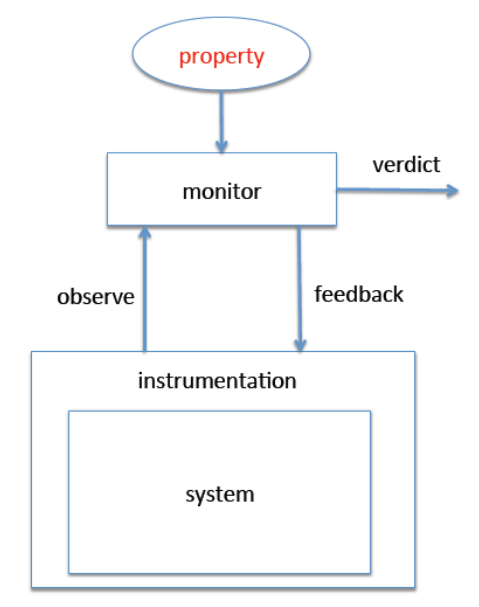
\includegraphics[width=80mm]{rvstruct.png}
\caption{Runtime verification process (from \cite{falcone2013tutorial})}
\label{img:rvstruct}
\end{center}
\end{figure}

Figure \ref{img:rvstruct} describes the process of a typical runtime verification system which contains the following four steps \citep{falcone2013tutorial}:
\begin{enumerate}
\item \emph{Monitor synthesis}: A monitor is synthesized from a property.
\item \emph{System instrumentation}: Extra instruments are integrated with the system under scrutiny in order to generate the events for the \emph{monitor}.
\item \emph{Execution}: The system is executed and starts to generate events and send them to the monitor.
\item \emph{Analysis and response}: The monitor analyzes the collected events, emits a \emph{verdict} and sends additional information, i.e. \emph{feedback} to the system if necessary.
\end{enumerate}

Monitors can be classified into several modes from different aspects \citep{chen2007mop}:
\begin{itemize}
\item \emph{online/offline} depends on when the monitors and the system work. \emph{Online} if they work at the same time, and \emph{offline} if the monitors start to work after the termination of the execution of the system.
\item \emph{inline/outline} depends on where the monitors are executed. \emph{inline} if the monitors are embedded into the system and \emph{outline} if the monitors run all alone while receiving the event traces from the system by certain methods, e.g. via file system or wireless signal.
\item \emph{violation/validation} is determined by the specification of the verdict.
\end{itemize}

From the definitions of the modes, we can see that a monitor working in offline mode is also working in outline mode and the inline mode implies the online mode.

\subsection{Comparison with other techniques}

Comparing with model checking \citep{clarke1999model} which aims to verify finite state systems, the methods of generating monitors in runtime verification and generating automatas in model checking have similarities. However, whereas model checking deals mainly with infinite traces, runtime verification deals only with finite traces, i.e. the executions. For this reason, the monitors of runtime verification working in online monitoring mode have to be able to accept incremental traces.

Another important difference between model checking and runtime verification is that, unlike model checking which checks if all executions of a system satisfy a correctness property, runtime verification is interested only with whether existing an execution which belongs to a set of valid executions. Moreover, runtime verification only requires to analyze the observed events of a given system without having to watch its internal running information, but in model checking, the proper model of the system must be acknowledged in order to prepare every possible execution before running the system. \citep{leucker2009brief}

Software testing \citep{broy2005model} is another verification technique. It is a process of running a program with a finite set of input-output sequences which is also namely test suite. Comparing with runtime verification, test suites are defined directly, unlike properties of runtime verification which are generated from formalism specification. Besides, ``exhaustive testing'' which is a common method in software testing, is normally not an option of runtime verification.

\section{Linear temporal logics}

In runtime verification, a monitor is translated from a correctness property, and correctness properties are specified in linear-time temporal logics, such as LTL.

Temporal logic is an extension of classical logic, and it provides a convenient language with the expressions of the properties to reason about the change of the states in terms of time. Although there are a lot of different temporal logics invented to meet various requirements, the temporal logics are normally classified by whether the time is linear or branching. The temporal logic with linear time is called \emph{Linear Temporal Logic} (LTL) which was first proposed by \cite{pnueli97}. Time in LTL is turned into a sequence of states which extend to the infinite future. The sequence of states is a computation \emph{path}. \citep{clarke1999model} \citep{huth2004}

\cite{leucker2009brief} summarizes LTL as a well-accepted linear-time temporal logic used to specify properties of infinite traces. However, in runtime verification, LTL is employed to check finite executions.

\subsection{Syntax}

A well-formed \emph{LTL} formula consists of a finite set of atomic propositions, boolean operators $\neg, \wedge, \vee, \rightarrow$ and temporal logic operators \textbf{F}(future), \textbf{G}(global), \textbf{X}(next), \textbf{U}(until), \textbf{W}(weak-until) and \textbf{R}(release). It can be represented in the Backus Naur form as follows \citep{huth2004}:
\begin{align}
\phi ::= & \top | \bot | p | (\neg\phi) | (\phi \wedge \phi) | (\phi \vee \phi) | (\phi \rightarrow \phi) \nonumber \\
& | (\X \phi) | (\F \phi) | (\G \phi) | (\phi \U \phi) | (\phi \W \phi) | (\phi \R \phi)
\end{align}

\subsection{Semantics}

For a sequence of states $s_0, s_1, s_2, ..., s_i, s_{i + 1}, ...$ where $s_{i + 1}$ is a future state of $s_i$, we define a path with $\pi^i = s_i \rightarrow s_{i + 1} \rightarrow ...$ where $i$ is the first state in this path. Given that $\pi(i)$ is the set of atomic propositions which are true at the $i$th state, whether a path $\pi^i$ satisfies an \emph{LTL} formula is defined as follows \citep{rozier2011linear}:

\begin{itemize}
  \item \listequation{\pi^i \vDash \top} \label{eq:true}
  \item \listequation{\pi^i \nvDash \bot} \label{eq:false}
  \item \listequation{\pi^i \vDash p \iff p \in \pi(i)} \label{eq:ap}
  \item \listequation{\pi^i \vDash \neg\psi \iff \pi^i \nvDash \psi} \label{eq:not}
  \item \listequation{\pi^i \vDash \psi \wedge \varphi \iff \pi^i \vDash \psi \text{ and } \pi^i \vDash \varphi} \label{eq:and}
  \item \listequation{\pi^i \vDash \psi \vee \varphi \iff \pi^i \vDash \psi \text{ or } \pi^i \vDash \varphi} \label{eq:or}
  \item \listequation{\pi^i \vDash \psi \rightarrow \varphi \iff \pi^i \vDash \varphi \text{ whenever } \pi^i \vDash \psi} \label{eq:then}
  \item \listequation{\pi^i \vDash \X \psi \iff \pi^{i + 1} \vDash \psi} \label{eq:next}
  \item \listequation{\pi^i \vDash \G \psi \iff \forall j \geq i, \pi^j \vDash \psi} \label{eq:global}
  \item \listequation{\pi^i \vDash \F \psi \iff \exists j \geq i, \pi^j \vDash \psi} \label{eq:future}
  \item \listequation{\pi^i \vDash \psi \U \varphi \iff \exists j \geq i, \pi^j \vDash \varphi$ and $\forall k, i \leq k < j, \pi^k \vDash \psi} \label{eq:until}
  \item \listequation{\pi^i \vDash \psi \W \varphi \iff$ either $\exists j \geq i, \pi^j \vDash \varphi$ and $\forall k, i \leq k < j, \pi^k \vDash \psi$, or $\forall k \geq i, \pi^k \vDash \psi} \label{eq:wuntil}
  \item \listequation{\pi^i \vDash \psi \R \varphi \iff$ either $\exists j \geq i, \pi^j \vDash \psi$ and $\forall k, i \leq k \leq j, \pi^k \vDash \varphi$, or $\forall k \geq i, \pi^k \vDash \varphi} \label{eq:release}
\end{itemize}

Formul\ae{}s \ref{eq:true} and \ref{eq:false} suggest that the states in the path $\pi^i$ should be always true or false.

In formul\ae{} \ref{eq:ap}, $p$ is an atomic proposition belonging to the finite set of atomic propositions of LTL, and this formul\ae{} demands to check only the $i$th state.

Formul\ae{}s \ref{eq:not}---\ref{eq:then} are boolean operators of propositional logic following the rules of Table \ref{table:prologic}

\begin{table}[h]
\centering
\begin{tabular}{|c|c|c|c|c|c|}
\hline
$\psi$ & $\varphi$ & $\neg\psi$ & $\psi \wedge \varphi$ & $\psi \vee \varphi$ & $\psi \rightarrow \varphi$ \\
\hline
True & True & False & True & True & True \\
\hline
True & False & False & False & True & False \\
\hline
False & True & True & False & True & True \\
\hline
False & False & True & False & True & True \\
\hline
\end{tabular}
\caption{The truth table of boolean operators of propositional logic}
\label{table:prologic}
\end{table}

Formul\ae{}s \ref{eq:next}, \ref{eq:future} and \ref{eq:global} are unary temporal logic connectives.
\X means ``next time'' and it skips the $i$th state and evaluates the path $\pi^{i+1}$. \F stands for ``sometimes in the future'' which requires that from the $i$th state, a property holds in a future state on the path. And \G (``globally'' or ``always'') denotes that a property should hold on the every state from the $i$th state until the end or the infinite future.

Formul\ae{}s \ref{eq:until}, \ref{eq:wuntil} and \ref{eq:release} are binary temporal logic operators. \U is the abbreviation of ``until''. The formul\ae{} $\psi \U \varphi$ holds if $\varphi$ holds at a future state on the path, and before this state the property $\psi$ holds at every state. \W, ``weak-until'', is a weak version of \U, except that for the formul\ae{} $\psi \W \varphi$, $\varphi$ does not have to hold eventually in some future state. \R, which stands for ``release'', is actually a logic dual of \U, i.e. $\psi \U \varphi \equiv \neg(\neg\psi \R \neg\varphi)$. \R requires that for the formul\ae{} $\psi \R \varphi$, the property $\varphi$ should hold continuously until $psi$ holds or $psi$ does not hold eventually.

It is worth noting that in LTL, the two-valued logics might yield a premature result which is either true or false. As is mentioned above, LTL is defined to work with infinite traces whereas monitoring of runtime verification is only able to treat finite traces, which might lead to a conflict, especially in some running system. For instance, $\F \psi$ states that $\psi$ should hold in a future state. In a running system, as long as $\psi$ does not hold in the observed states, the results of the formul\ae{} are always $false$, but if $\psi$ holds in the next observation, the former results will become corrupted and obsolete. Therefore, \cite{bauer2006monitoring} proposed the three-valued logic LTL$_3$ which introduces an new value \emph{inconclusive} for the cases where the property cannot be evaluated immediately.

\subsection{Various LTLs}

\subsubsection{Metric Temporal Logic}

Metric Temporal Logic (MTL) \citep{chang1994compositional} was invented to reason about real-time properties. To precise time accurately, MTL cuts the time into numbered pieces which is also called timed transition modules, and employs boundary operators to constrain the temporal logic operators. Its formul\ae{} is defined as follows:
\begin{align*}
\phi ::= & \bot | p | (\phi \rightarrow \phi) | (\fullmoon_{\sim{}c}\phi) | (\circleddash_{\sim{}c}\phi) | (\phi \mathrel{U}_{\sim{}c} \phi) | (\phi \mathrel{S}_{\sim{}c} \phi) \\
& \mbox{where } \sim \in \{<, =, >, \equiv_d\} \mbox{ and } c \geq 0, d \geq 2
\end{align*}

$\fullmoon_{\sim{}c}\phi$ means ``Next'', $\circleddash_{\sim{}c}\phi$ means ``Previous'', $\phi \mathrel{U}_{\sim{}c} \phi$ means ``Until'' and $\phi \mathrel{S}_{\sim{}c} \phi$ means ``Since'' \citep{chang1994compositional}. Given that $T_i$ indicates the time of the $i$th state of the path $\pi^i$, whether a formul\ae{} holds at the position $j$ of the path $\pi$ is defined as follows (we ignore the propositional operators here):
\begin{eqnarray*}
\pi^i \vDash \fullmoon_{\sim{}c}\psi & \iff & \pi^{i+1} \vDash \psi \mbox{ and } T_{i+1} - T_i \sim c \\
\pi^i \vDash \circleddash_{\sim{}c}\psi & \iff & i \geq 1 \mbox{ and } \pi^{i-1} \vDash \psi \mbox{ and } T_i - T_{i-1} \sim c \\
\pi^i \vDash \psi \mathrel{U}_{\sim{}c} \varphi & \iff & \exists j \mbox{ where } i \leq j, \pi^j \vDash \varphi \mbox{ and } T_k - T_j \sim c, and \forall k \mbox{ where } i \leq k < j, \pi^k \vDash \psi \\
\pi^i \vDash \psi \mathrel{S}_{\sim{}c} \varphi & \iff & \exists j \mbox{ where } 0 \leq j \leq i, \pi^j \vDash \varphi \mbox{ and } T_j - T_k \sim c, and \forall k \mbox{ where } j < k \leq j, \pi^k \vDash \psi \\
\end{eqnarray*}

\subsubsection{Past time LTL}

Whereas LTL mentioned in the last part is defined to check the future states, Past time LTL (ptLTL) aims to verify the states in the past. A ptLTL formul\ae{} is defined as follows \citep{havelund2004efficient}:
\begin{align*}
\phi ::= & \top | \bot | p | (\neg\phi) | (\phi \wedge \phi) | (\phi \vee \phi) | (\phi \rightarrow \phi) \\
& | (\odot \phi) | (\diamond \phi) | (\boxdot \phi) | (\phi \mathrel{S_s} \phi) | (\phi \mathrel{S_w} \phi) \\
& | (\uparrow \phi) | (\downarrow \phi) | [\phi, \phi)_s | [\phi, \phi)_w
\end{align*}

As can be seen in the definition of the formul\ae{}, ptLTL keeps several basic operators as LTL and introduces five standard part time operators and four monitoring operators.

The five standard part time operators are $\odot $ which means ``previous'', $\diamond$ ``eventually in the past'', $\boxdot$ ``always in the past'', $\mathrel{S_s}$ ``strong since'' and $\mathrel{S_w}$ ``weak since''.

The monitoring operators $\uparrow \downarrow [,)_s [,)_w$ mean respectively ``start'', ``end'', ``strong  interval'' and ``weak  interval''.

The temporal operators' semantics are described as follows, in the same form of the last section:
\begin{eqnarray*}
\pi^i \vDash \odot \psi & \iff & \mbox{ if } i > 0, \pi^{i - 1} \vDash \psi, or \mbox{ if } i = 0, \pi^0 \vDash \psi \\
\pi^i \vDash \diamond \psi & \iff & i > 0 \mbox{ and } \exists j \mbox{ where } 0 \leq j \leq i, \pi^j \vDash \psi \\
\pi^i \vDash \boxdot \psi & \iff & i > 0 \mbox{ and } \forall j \mbox{ where } 0 \leq j \leq i, \pi^j \vDash \psi \\
\pi^i \vDash \psi \mathrel{S_s} \varphi & \iff & \exists 0 \leq j \leq i, \pi^j \vDash \varphi \mbox{ and } \forall k, j < k \leq i, \pi^k \vDash \psi \\
\pi^i \vDash \psi \mathrel{S_w} \varphi & \iff & \pi^i \vDash \psi \mathrel{S_s} \varphi \mbox{ or } \pi^i \vDash \boxdot\psi \\
\pi^i \vDash \uparrow \psi & \iff & \pi^i \vDash \psi \mbox{ and } \pi^{i - 1} \nvDash \psi \\
\pi^i \vDash \downarrow \psi & \iff & \pi^i \nvDash \psi \mbox{ and } \pi^{i - 1} \vDash \psi \\
\pi^i \vDash [\psi, \varphi)_s & \iff & \exists j \mbox{ where } 0 \leq j \leq i, \pi^j \vDash \psi, \mbox{ and } \forall k \mbox{ where } j \leq k \leq i, \pi^k \nvDash \varphi \\
\pi^i \vDash [\psi, \varphi)_w & \iff & \pi^i \vDash [\psi, \varphi)_s \mbox{ or } \pi^i \vDash \boxdot\neg\varphi \\
\end{eqnarray*}

\subsubsection{EAGLE}

EAGLE \citep{barringer2004rule} is a temporal finite trace monitoring logic supporting parameterized equations by combining minimal/maximal fix-point semantics with temporal operators.

Online runtime verification requires to accept incremental traces which means there are possible boundaries between traces. Minimal/maximal fix-point rules were designed to treat this problem. Before evaluating the next trace, the equations with maximal rules are required to be always right and the ones with minimal rules are only needed to be eventually right.

\section{Runtime verification frameworks}\label{sec:rv:frameworks}

In runtime verification, monitors are generated from formal specifications by runtime verification frameworks. There are four monitoring modes: offline, online, inline and outline as we discussed in the early part of this section. Many frameworks and systems using some variant or extension of LTL have been proposed, as Table \ref{table:rvframeworks} shows. 

\begin{table}[h]
\centering
\begin{tabular}{|c|c|c|}
\hline
Name & Logic & Mode \\
\hline
JPax\citep{havelund2001java} & LTL \& Past-time LTL & outline \\
\hline
JavaMaC\citep{kim2004java} & Past-time LTL & outline \\
\hline
Hawk \citep{d2005event} & Hawk & outline \\
\hline
Temporal Rover\citep{drusinsky2000temporal} & LTL \& MTL & outline \\
\hline
MOP \citep{chen2007mop} & Various & inline/outline/offline \\
\hline
\end{tabular}
\caption{Runtime Verification Frameworks}
\label{table:rvframeworks}
\end{table}

Java PathExplorer (JPaX) \citep{havelund2001java} is an online runtime verification system aiming to monitor the execution traces of Java program. It has three modules (shown in Figure \ref{img:jpax}): an instrumentation module, an observe module and an interconnection module. The program working with the instrumentation module sends necessary event traces to the interconnection module which then transmits the traces to the observe module possibly running on another computer. The instrumentation module is driven by a user-specified script written in Java or Maude which is applicable for the specification of runtime monitoring.

\begin{figure}[h]
\begin{center}
\centering
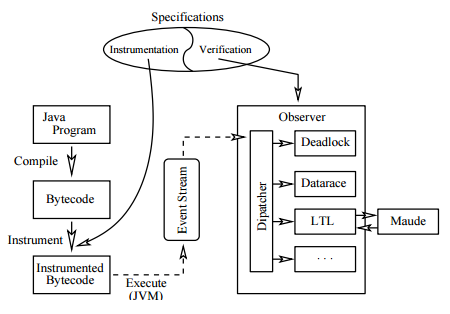
\includegraphics[width=100mm]{jpax.png}
\caption{JPaX Architecture (from \cite{havelund2001java})}
\label{img:jpax}
\end{center}
\end{figure}

JavaMaC \citep{kim2004java} is a ``run-time assurance system'' for Java programs while Mac means Monitoring and Checking. Its architecture is shown in Figure \ref{img:javamac}. Two definition languages are proposed: one for high-level specification which specifies required properties, another for low-level specification which defines the events and conditions. During the preparation, a ``filter'' and an ``event recognizer'' which are used to collect the necessary event traces are generated from the low-level specification, and a ``run-time checker'' is generated from the high-level spec. When running with the target program, events collected by the ``filter'' and ``event recognizer'' are sent to the ``run-time'' checker which is then responsible for the runtime verification work.

\begin{figure}[h]
\begin{center}
\centering
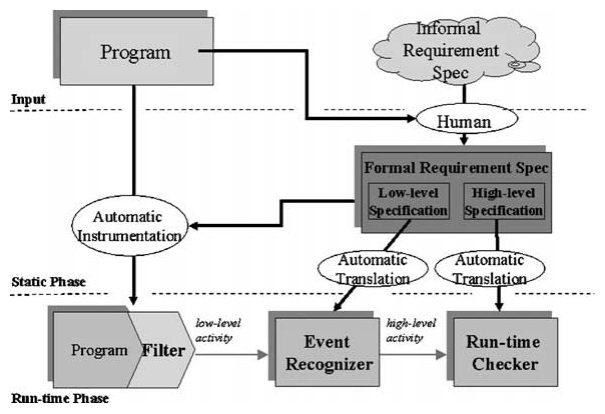
\includegraphics[width=100mm]{javamac.png}
\caption{MaC Architecture (from \cite{kim2004java})}
\label{img:javamac}
\end{center}
\end{figure}

\cite{d2005event} presents a logic named HAWK and its tools for RV of Java programs. HAWK is in fact built on EAGLE, another temporal logic which is considered more expressive \citep{barringer2004rule}. Although HAWK is event-based in contrast to state-based EAGLE, HAWK specifications are translated to EAGLE monitors. As Figure \ref{img:eagle} describes, during program execution, the EAGLE state is updated by instrumented program which then notifies the EAGLE observer. After that, the observer assesses the formul\ae{} in the current state to produce a result. 

\begin{figure}[h]
\begin{center}
\centering
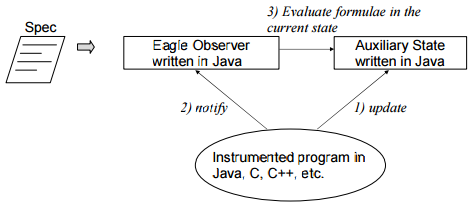
\includegraphics[width=100mm]{eagle.png}
\caption{Eagle Architecture (from \cite{d2005event})}
\label{img:eagle}
\end{center}
\end{figure}

Temporal Rover \citep{drusinsky2000temporal} is a commercial runtime verification tool based on LTL and MTL (Metric Temporal Logic). The specification code of Temporal Rover is inserted into the source code of Java, C, C++ or HDL and then converted into a compilable source file of corresponding language. A Temporal-Rover runtime verification system normally has two parts: host and target. The host is responsible for the verification while the target performs the computation of propositional formul\ae{} and sends back the results to the host via serial port, RPC or other customizable protocol.

Each of the frameworks discussed above hardwires a different specification formalism, which suggests that a general specification formalism serving all purposes does not exist. To be more expressive and generic, \cite{chen2007mop} introduced customizable and extensible ``logic-plugins'' in their runtime framework MOP and designed its architecture shown in Figure \ref{img:mop} with two layers: one is called ``language clients'' which support different programming languages, while another is ``logic repository'' which includes and manages various ``logic-plugins'' to support different specification formalisms, such as : Linear Temporal Logic (ltl), Finite State Machines (fsm), Extended Regular Expressions (ere), Context Free Grammars (cfg) and String Rewriting Systems (srs).

\begin{figure}[h]
\begin{center}
\centering
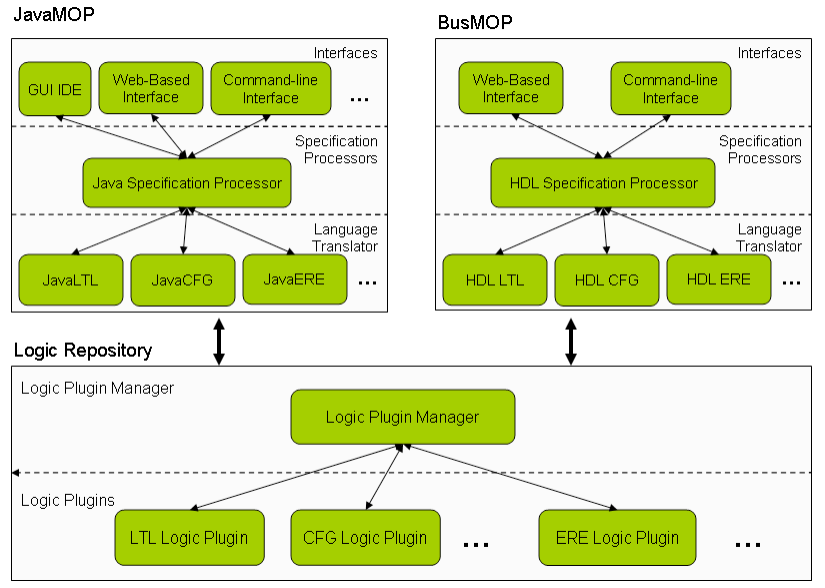
\includegraphics[width=130mm]{mop.png}
\caption{MOP Architecture (from \cite{chen2007mop})}
\label{img:mop}
\end{center}
\end{figure}

Besides the frameworks presented above, there are also lots of other frameworks invented for their corresponding requirements or specific temporal logics. Comparing these frameworks, we can find that they have their specialties as well as they share some common characters. For example, nearly all frameworks support online monitoring mode, Java programming language and network communication perhaps because these features are the most popular requirement in industry. Temporal Rover is a commercial RV framework, so it has to support more programming languages and supply more data collection options in order to expand its marketing. MOP was designed to be extremely general, resulting that most components can be changed or separately optimized.

\chapter{Real-Time Streaming Communication with Optical Codes}
\vspace*{\fill}{This chapter represents a modified version of a paper published in 2016 in IEEE Access, v.4, p. 284-298 by K. Xie and S. Gaboury and S. Hallé.\clearpage}

\section*{Abstract}
Optical codes have long been used to carry small amounts of static data, such as URLs, IDs or other short binary sequences. In this chapter, we experiment on the use of sequences of optical codes to form a one-way communication channel. In this context, a sender is made of a surface displaying rapidly changing codes, which are picked up by a receiver's camera and converted back into a binary data stream. After presenting experimental results seeking the combination of frame rate, code size and error correction level maximizing effective bandwidth, we describe the implementation of a robust communication protocol designed specifically for lossy, simplex, and low-bandwidth data links. Our findings indicates that such a protocol is sufficient for carrying at least voice-quality audio in realtime.

%% -----------------------
%% Section: intro
%% -----------------------
\section{Introduction}\label{sec:qr:intro} %% {{{

Wireless communication is a technology that allows two or more peers to communicate without electric cables or conductors \cite{tse2005fundamentals}. While the majority of wireless communication technologies uses radio waves as their transmission medium, a few others use light, especially in situations where radio technology is difficult to apply. Optical communication in itself reaches back to the use of flags, smoke signals and signal lamps to communicate information between two points with the use of a specific code~\cite{burns2004}.

Recently, a simple form of optical communication, called \emph{Quick Response Code} (QR code) \cite{qrcode-about}, emerged as a refinement over the existing technology of one-dimensional barcodes. Owing to their accuracy and their considerable capacity, QR codes have been used in many areas; applications for handling such codes have also been ported to a variety of devices, including desktop computers, smartphones, and even television sets.

However, so far QR codes have been used for the transmission of \emph{static} data. Generally a code is printed on a physical medium, such as a sheet of paper, and is read by an optical device (typically a camera) for decoding at a later time. In this chapter, we explore the idea of extending QR codes and turn them into a dynamic, one-way communication channel. In such a channel, a stream of data is transmitted through a \emph{sequence} of codes; typically, these codes are continuously generated and displayed on one device, and simultaneously captured and decoded by another, hence performing the same task as other kinds of communication technologies.

After briefly describing in Section~\ref{sec:qr:reading} the basics of QR codes and other wireless communication technologies, we shift our focus in Section~\ref{sec:qr:qrcode} to the principle of raw QR code communication. In particular, we attempt to find the intrinsic limits of such a communication channel, by analyzing the influence of a variety of factors, such as code density, number of codes displayed per second, etc. The results of an experimental benchmark considering more than a hundred different combinations of parameters allow us to extract optimal conditions that minimize the rate of error in decoding the images, while maximizing the amount of data that can be transmitted per unit of time.

%The code decoding depends on the quality and the complexity of the captured image. If the image is broken or blurred, it will be difficult to decode. And the algorithms of image recognition may have the probability of failure\cite{adel2006}. Therefore, at first, we did a benchmark with combinations of the parameters, such as the camera configuration, the frame rate, and the data size in one code. According to the benchmark result, we selected an optimal combination for our second step.

These first results indicate that QR code streams can indeed be used as a simple, one-way channel, but that error-free communication and high-bandwidth are more or less impossible. Therefore, as a second step, we design a protocol suitable for the specific nature of QR code communication. This protocol, called BufferTannen, is described in Section~\ref{sec:qr:protocol}. It is able to encapsulate raw data, provides various signaling capabilities, can represent semi-structured data (such as JSON) in a compact binary form, and supports data framing/deframing and streaming.

A second experiment reveals the robustness of this transmission scheme: using our specially designed protocol, the communication channel created by a person pointing a smartphone at arm's length towards a flickering QR display produces sufficient bandwidth to transmit voice-quality audio in real time. Section~\ref{sec:qr:experiments} presents the environment and the results of the experiments of this second step. We also show how a piece of data, cut into multiple codes with the use of BufferTannen, can be reconstructed automatically by a user hovering his camera over a sheet of such printed codes in no particular order.

This work was originally motivated by a practical application in the field of runtime verification. In past research, we suggested and informally experimented the use of optical codes as a form of loosely coupled communication between a software system and an external monitor receiving events produced by that system \cite{DBLP_conf/rv/LavoieLVGH14}. In this context, communication through optical means ensured a complete isolation between the system and its monitor.

Although the use of sequences of QR codes has been informally suggested in the past, to the best of our knowledge, our study is the first systematical investigation of the potential of QR codes to send streams of data in real time. %Because QR codes are basically images, besides being displayed on the screen, they can be also distributed in other ways, for example, they can be printed on the papers or other printable surfaces. 

The solution we propose provides a method for distributing streaming data without dedicated communication devices. The only required devices are a common camera (such as a webcam or the camera on any cellphone) and a small flat surface to display the sequential QR codes ---for example, a computer, television or smartphone screen, or even a sheet of paper.

%% }}} --- Section

%% -----------------------
%% Section: comment on lit les codes QR
%% -----------------------
\section{Wireless Communications}\label{sec:qr:reading} %% {{{

This section recalls a few common wireless communication technologies. Despite their popularity and performance, each has its own limitations and application scenarios. %, which leads to our problematic: find another communicating solution and prove its feasibility.

\subsection{Radio Waves}

The first obvious means of wireless communication is through the use of radio waves, and is best exemplified through WiFi \cite{Comer:2008:CNI:1816918}, used for local area wireless networking. Its variants are based on the IEEE 802.11 family of standards, and support both centralized (routing) and decentralized (\textit{ad hoc}) networking. Table \ref{tab:qr:wifi-protocol} shows popular 802.11 standards and part of their specifications.

\begin{table}[ht]
\begin{center}
\begin{tabular}{|l|l|l|l|}
\hline
Protocol &	Frequency & 	Max. physical data rate &	Indoor range\\
\hline
802.11a &	5 GHz &	54 Mbps &	35 m \\
\hline
802.11b &	2.4 GHz &	11 Mbps &	35 m\\
\hline
802.11g &	2.4 GHz &	54 Mbps &	38 m\\
\hline
802.11n &	2.4/5 GHz &	150 Mbps &	70 m\\
\hline
802.11ac &	5 GHz &	866.7 Mbps & 35 m\\
\hline
\end{tabular}
\caption{A summary of WiFi protocols\cite{theng2008ubiquitous,perahia2013next}}
\label{tab:qr:wifi-protocol}
\end{center}
\end{table}

A second contender in this family is Bluetooth \cite{Comer:2008:CNI:1816918}, which is used for short-range and generally point-to-point communication between devices. Its range varies from about 1 to 100 meters depending on the class of power. Table \ref{tab:qr:bluetooth} shows different versions of Bluetooth and their specific data rates.

\begin{table}[ht]
\begin{center}
\begin{tabular}{|l|r|c|}
\hline
Version &	Data rate	&	Range\\
\hline
Version 1.2 &	1 Mbps &	\multirow{4}{*}{\pbox{20\textwidth}{Class 1: 100 m; \\ Class 2: 10 m; \\ Class 3: 1 m}}\\
\cline{1-2}
Version 2.0 + EDR &	3 Mbps & \\
\cline{1-2}
Version 3.0 + HS &	24 Mbps & \\
\cline{1-2}
Version 4.0 &	24 Mbps & \\
\hline
\end{tabular}
\caption{Bluetooth specifications \cite{gupta2013inside}}
\label{tab:qr:bluetooth}
\end{center}
\end{table}

Finally, ZigBee \cite{farahani2011zigbee}, based on the IEEE 802.15.4 standard, aims to implement short-range wireless communication with low power and long battery life. Table \ref{tab:qr:zigbee} shows its performance in different frequency bands.

\begin{table}[ht]
\begin{center}
\begin{tabular}{|l|r|c|}
\hline
Frequency Band  &	Data rate	&	Range\\
\hline
868--870 MHz &	20 kbps &	\multirow{3}{*}{\pbox{3cm}{10--100 m, depending on power output and environment}}\\
\cline{1-2}
902--928 MHz &	40 kbps & \\
\cline{1-2}
2.4--2.4835 GHz  &	250 kbps & \\
\hline
\end{tabular}
\caption{ZigBee specifications \cite{lee2007comparative}}
\label{tab:qr:zigbee}
\end{center}
\end{table}

All these protocols have on point in common: before allowing any form of communication between two endpoints, some form of \emph{discovery} or \emph{setup} of devices is necessary. This process is generally finalized through the establishment of a long-running and stateful \emph{connection} between the endpoints.

\subsection{IrDA}

In a different family, we find technologies using infrared waves instead of radio \cite{sarkar2007ad}. In addition to the different wavelength, these technologies generally relax the requirements on the establishment of a connection, and allow for a more ``on-the-fly'' communication between two devices. Typically, one end of an infrared link waits for incoming data, while periodically, another device ``points'' at the receiver and beams short bursts of data without requiring prior notice.

Of particular importance is the IrDA standard (Infrared Data Association); its transceivers send infrared pulses with a cone angle and a moderate irradiance while its receivers can be less than one meter or several meters away depending on the power of the transceivers and the position in the cone. The IrDA communication is half-duplex and provides basic CRC. Table \ref{tab:qr:irda-rate} shows several IrDA schemas and their data rates in the specific range.

\begin{table}[ht]
\begin{center}
\begin{tabular}{|l|c|c|}
\hline
Schema & Data rate & Range\\
\hline
SIR &	2.4--115.2 kbps &	\multirow{4}{*}{\pbox{3cm}{Up to one meter}} \\
\cline{1-2}
MIR &	0.576--1.152 Mbps & \\ 
\cline{1-2}
FIR &	4 Mbps & \\
\cline{1-2}
GigaIR &	512 Mbps--1 Gbps & \\
\hline
\end{tabular}
\caption{Data rates for IrDA Physical Layer schemas\cite{millar1998irda}}
\label{tab:qr:irda-rate}
\end{center}
\end{table}

\subsection{Visible Light Communication}

As its name implies, Visible Light Communication (VLC) \cite{komine2004fundamental} uses wavelengths in the visible range (from 400 to 700 nm) to communicate data between peers ---this is typically achieved by rapidly switching a light source on and off, enabling a form of Morse-like encoding of data. A receiver (such as a photo-electrical cell) pointed at the light source detects this flickering and converts it back into digital data. With fluorescent lamps as the light source, the data rate can reach 10 kbps, while with LED technology, the data rate can be as high as 500 Mbps.  The range depends mostly on different specifications, but because it cannot penetrate walls and can also be impacted by dense weather or other light sources, its range and reliability are limited~\cite{arnon2015visible}.

This mode of communication is intrinsically one-way, as one cannot reply back to the light source, acknowledge reception of information, or request for a retransmission in case of lost data. Therefore, this technology is also the one that requires the least coupling between a transmitter and a receiver; by all practical means, the transmitter is unaware of the presence of a receiver, which, on its side, may elect to start listening at any point in time. We shall see later on that this characteristic is also shared with the QR communication channel we attempt to design.

%% }}} --- Section

%% -----------------------
%% Section: le protocole
%% -----------------------
\section{Reading Streams of QR codes}\label{sec:qr:qrcode} %% {{{

Not mentioned in the previous short survey of wireless communication technologies are optical codes, which are also a means of carrying data without the need for a physical media. In this section, we review the concept of QR codes, and discuss the idea of producing streams of data through sequences of such codes.

\subsection{Overview of QR codes}

A QR code (officially called ``Quick Response Code'') \cite{qrcode-about} is a two-dimensional barcode that stores data, as shown in Figure \ref{fig:qr:helloqr}. Compared with the well-known UPC barcode, which is a linear (i.e.\ one-dimensional) barcode, a QR code can store more information in a smaller printout size.\footnote{\url{http://www.qrcode.com/en/}} The QR code standard stipulates that these codes can have a capacity as high as 7,089 numeric characters or 2,953 8-bit characters, represented in a square array of a maximum of 177$\times$177 ``pixels'', called \emph{modules} \cite{iso18004}. 

\begin{figure}
\centering

\includegraphics[width=1in]{helloqr.png}
\caption{A QR code with the text ``Hello world!''}
\label{fig:qr:helloqr}
\end{figure}

\begin{table}[t]
\begin{center}
\begin{tabular}{|l|l|l|l|l|l|}
\hline
\pbox[c][25pt][c]{\textwidth}{Error correction \\level} & Data bits & Numeric &	Alphanumeric & Binary & Kanji\\
\hline
L &	23,648 & 7,089 & 4,296 & 2,953 & 1,817\\
\hline
M & 18,672 & 5,596 & 3,391 & 2,331 & 1,435\\
\hline
Q & 13,328 & 3,993 & 2,420 & 1,663 & 1,024\\
\hline
H & 10,208 & 3,057 & 1,852 & 1,273 & 784\\
\hline
\end{tabular}
\caption[Capacities]{Maximum storage capacities for Version-40 codes}
\label{tab:qr:qrcode-capacity}
\end{center}
\end{table}

The capacity of a QR code mainly depends on its data type, version and error correction level. The data type can be \emph{Numeric only},  \emph{Alphanumeric},  \emph{Binary}, or \emph{Kanji}. The version, from 1 to 40, determines a code's dimensions, which range from 21$\times$21 to 177$\times$177 modules. QR codes use a form of error-correction coding which can take four levels: \emph{Low} (L),  \emph{Medium} (M),  \emph{Quartile} (Q), and  \emph{High} (H), as is shown in Table~\ref{tab:qr:qrcode-capacity}. Obviously, as the level increases, more redundancy is introduced in the code's content, which decreases its storage capacity; however, more data can be restored if the code is dirty or damaged. With position detection patterns included in the symbol, a QR code can be decoded in 360 degrees.

Before generating a QR code from a piece of data, a code generator needs to analyze that input data to decide the most efficient mode and version. In the data encoding, the characters are converted into a bit stream, and in this progress, some \emph{mode indicators} and \emph{terminators} are inserted for the mode changes. The bit stream is then split into 8-bit codewords, and pad characters are required to fill the number of codewords for the chosen version. The generated codeword sequence is divided into blocks according to the specific error correction level and an error correction codeword is generated for each block. Then the codewords from each block are interleaved and some remainder bits are added as necessary.

In the next step, the generator places the codeword modules in a black-and-white matrix with the finder pattern, separators, timing pattern and alignment Patterns; it applies the masking patterns, evaluates and then selects the appropriate pattern. Finally, it generates the \emph{Format} and \emph{Version Information} and completes the QR code \cite{iso18004}.

The decoding steps are simply the reverse of the encoding procedure. At first, the QR code needs to be located and the black and white modules are recognized as 0s and 1s that form a binary array. From the binary array, the decoder gets the format information and version information. With that information, it can begin to read the characters and the error correction codewords, and then tries to detect and correct the errors with the error correction codewords according to the appropriate error correction level. In the next step, the data codewords are divided according to the \emph{Mode Indicators} and \emph{Character Count Indicators}, and the data characters are finally decoded and output.

\subsection{The Case for QR code Communication}

The aforementioned process applies for the encoding and decoding of a single code containing static data. We now investigate the idea of using QR codes as a communication channel, where realtime data would be transformed on-the-fly as a \emph{sequence} of QR codes, which could then be optically picked up by some device, and converted back into the original data stream at the receiving end.

The use of QR code communication presents several advantages in a handful of scenarios. For example, the US Navy has investigated the use of QR codes as a ``digital semaphore''. The proposed technology focuses on the detection of low-resolution codes from very long ranges, and highlights the interest and possible use cases for this technology in a military context:

\begin{quote}
Arguably the most significant advantage of QR code LOS [line of sight] communications is the fact that they can be conducted without emitting energy in the RF spectrum. In an emissions controlled (EMCON) environment, this will provide a critical ability to communicate between ships without increasing the possibility of position detection. \cite[p.\ 46]{richter-msc}
\end{quote}

However, in the cited work, the codes are considered to be \emph{static}, i.e.\ they do not change over time to form a stream of data, and more or less act as a substitute for flags or signs. Nevertheless, the absence of any emission of radio waves in QR code communication proves to be an appealing advantage in some scenarios.

We have also seen in the previous section how all other technologies, such as  Bluetooth or IrDA, require dedicated hardware. In contrast, using QR codes to communicate can be done through codes printed on a hard surface, or through any device capable of displaying images in sufficient resolution: TV screens, computer monitors, tablets and cell phones. Similarly, reception can be done through any device equipped with a standard, off-the-shelf camera. This can turn devices equipped with this common hardware into communicating devices, even though they were not designed for that purpose in the first place. One can even imagine emergency situations in which all digital means of communications between two points are not working. If line of sight can be established and a display and a camera are available, the use of QR codes nevertheless makes it possible to transmit digital data ---arguably much faster than the manual handwriting/transcribing that would otherwise need to be done.

\begin{comment}
Preliminary experiments show the technique can work on an inexpensive webcam with a low resolution of $640\times480$ (0.3 megapixels).
\end{comment}

Finally, we have mentioned in the beginning how the use of an optical and strictly one-way communication channel can also be desirable, even in situations where radio or cable communication is available. For example, in the context of runtime verification, the execution of a system is being observed by an external  process called a \emph{monitor}. To prevent the monitor from interfering with the execution of the system, it is often placed on a separate machine, with some communication channel carrying events from the former to the latter. However, in traditional protocols such as TCP, the bidirectional nature of a connection presents too high a risk of attacks on the program to monitor. Moreover, some software setup is required to hook up the monitor to the program: defining IP addresses, pipe names, ports, etc., which represents too much coupling in many scenarios. We have argued in past work \cite{DBLP_conf/rv/LavoieLVGH14} how the use of an optical communication channel can alleviate these problems by providing greater isolation between the system and its monitor.

\subsection{Estimating Bandwidth and Error Rate}

However, one-way transmission introduces the possibility of losing frames during the process, due to the limitation of the physical devices or the vulnerability of the software. Moreover, it is impossible for the transmitter to be aware of any missing frames on the receiving end and resend them. Therefore, we need to analyze thoroughly this approach to estimate the \emph{recognition rate} and the \emph{transmission bandwidth} of such a communication channel.

The transmission of codes takes multiple parameters: each frame's data size, the number of generated frames per second (fps) and the error correction level. All three can have an important effect on the generation of QR codes and the resulting bandwidth. Larger data size leads to a higher symbol version of the QR code and more symbol modules, and with the same frame size, a higher correction level requires more symbol modules than a lower one.

Because the sender cannot be aware of any codes missed by the receiver, this one-way communication channel is actually a lossy channel, of which the \emph{effective} bandwidth can be calculated with the measured frame recognition rate. This represents the number of bits that are correctly received.
%
\begin{equation*}
  bandwidth = \mathit{fps} \times \mathit{frame\_bits} \times \mathit{recognition\_rate}
\end{equation*}

If the receiver finds that not all the frames are received, the only way is to make sure the sender sends all the frames again and again until the receiver gets all frames and stops; the actual bandwidth is:
%
\begin{equation*}
  bandwidth = \mathit{fps} \times \mathit{frame\_bits} \div \mathit{actual\_sent\_times}
\end{equation*}

The recognition rate is normally determined by the ability of the camera and the screen, the accuracy of the recognition algorithm and the code's complexity (i.e.\ the number of the displayed modules). However, within the ability of the camera and the screen, if we can send the same frame for more than once, meanwhile the value of \emph{fps} doesn't need to change, the practical recognition rate can be improved.

\begin{equation*}
\mathit{practical\_recognition\_rate} = 1 - (1 - \mathit{recognition\_rate})^{times}
\end{equation*}


%% }}} --- Section

%% -----------------------
%% Section: expériences
%% -----------------------
\section{Experiments}\label{sec:qr:experiments} %% {{{

In this section, we describe experiments in which we measure the accuracy of reading sequences of QR codes in various conditions. The purpose of these experiments is threefold:

\begin{enumerate}
\item assess whether data can be successfully transmitted through the reading of sequences of optical codes;
\item determine the parameters that maximize the decoding rate and bandwidth of the transmitted data;
\item from these results, determine the characteristics of a typical QR stream communication channel.
\end{enumerate}

\subsection{Experimental Setup}

Our set of experiments involves producing and displaying sequences of QR codes on one end, and capturing and decoding these sequences on the other. In our experimental environment, we used a Samsung 19-inch LED monitor as the transmitter and a high-definition Logitech webcam as the receiver. The camera was placed at a fixed distance of 50 cm from the screen. The resolution of the monitor was 1280$\times$1024 pixels. %The webcam can capture at most 30 frames per second with the highest resolution of 1920 pixels $\times$ 1080 pixels. Zooming was disabled. 
The camera was placed on a stable surface, with the optical code zone correctly in focus and covering the whole field of view. The computer used for the experiments is a laptop with the Intel Core i7-3632QM processor and 16 GB of memory. Figure \ref{fig:qr:setup} shows the setup used for the experiments.

\begin{figure}
\centering
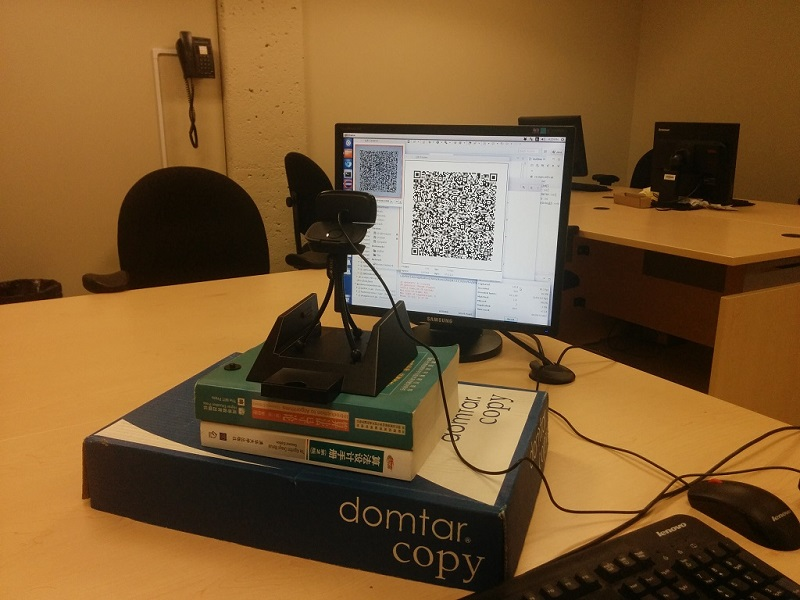
\includegraphics[width=\linewidth]{expsetup.jpg}
\caption{Experimental setup for reading codes.}
\label{fig:qr:setup}
\end{figure}

In the development, we chose OpenCV\footnote{\url{http://opencv.org/}} to capture the images from the camera and ZXing\footnote{\url{https://github.com/zxing/zxing}} to generate and decode the QR codes. To reduce the CPU and memory's overhead of capturing and decoding, the captured images were transformed to 16-level grayscale. The data used to generate QR codes were randomly generated \emph{alphanumerics}. All benchmarking code is implemented in Java and is freely available.\footnote{\url{http://github.com/sylvainhalle/GyroGearloose}}

The code decoding depends on the quality and the complexity of the captured image. If the image is broken or blurred, it will be difficult to decode. And the algorithms of image recognition may have the probability of failure\cite{adel2006}. Therefore, our first step is to measure the ability of optical recognition libraries to properly read sequences of codes, irrespective of the actual data contained in these codes. Sequences of codes were generated by producing a character string of the form \verb+dddd#rrrr...+, where \verb+dddd+ is a sequential number starting from zero and incrementing by one on each successive code, and \verb+rrrr...+ is a random string of characters (different on each code) long enough to fill the code up to its maximum size. Each test consisted in filming the sequence of such codes and storing the sequential number of each correctly decoded image into a file. This allows us to determine the fraction of all codes that were correctly read; given the size of each code and the number of codes sent, this makes it possible to compute the bandwidth and decoding error rate.

Our experiments quickly tripped over what appears to be a bug in the ZXing image decoding library. When analyzing sequences of images captured by the camera to look for decoding errors, we discovered that a number of times, the decoding failed while the corresponding image seemed to have no apparent problem (no blurring, correct framing, etc.). Putting the offending codes back on screen and trying to properly decode them with the camera yielded no success, even after changing the code's size, the camera's position, lighting conditions, etc. This is all the more puzzling that codes immediately before and after the problematic one were correctly decoded in multiple frames, while being captured in the same conditions. Even sending the code's ``pure'' image directly back into the decoding algorithm, without going through a camera, produces a decoding error.

It therefore seems the library cannot recognize some of the codes it itself produces (Figure \ref{fig:qr:bad-code} shows such an example). This most probably indicates a bug in the library, which has persisted up to the latest version available at the time this chapter was written. Therefore, in the following, the reader should keep in mind that an unknown proportion of reading errors may be due to this purported bug, and not to the particular experimental conditions. This is the case, for example, for the gaps in the correction rate we shall observe in Figures \ref{img-exp1} and \ref{img-exp2}.

\begin{figure}
\centering
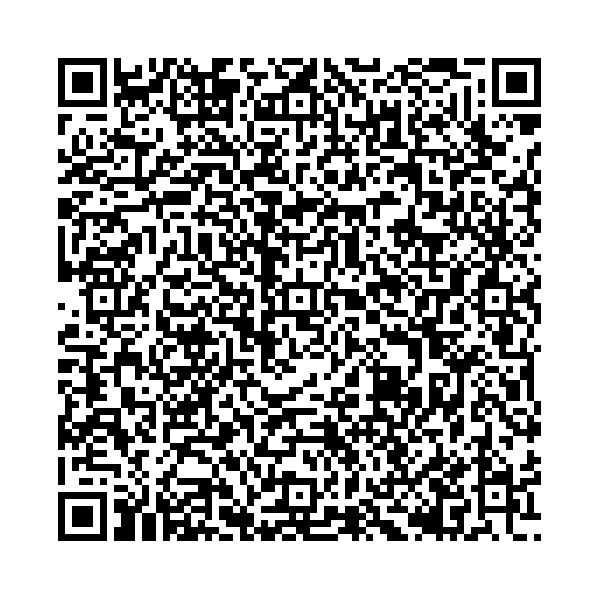
\includegraphics[width=.8\linewidth]{badqr.png}
\caption{A QR code generated by ZXing that ZXing itself cannot decode in the experiment.}
\label{fig:qr:bad-code}
\end{figure}

\subsection{Experimental Parameters}

The experiment seeks the combination of parameters that could maximize the bandwidth and minimize the error rate for the transmission of codes. The parameters that were considered are the following.

\subsubsection{Code Resolution}

The first parameter is code data size (i.e.\ the number of data bits contained in each code) and physical size (number of pixels used to display the code on screen). We varied the data size in increments of 500 bits, from 500 up to 4,500 bits. As shown in Table \ref{tab:qr:sample-sizes}, the largest QR code, which contains 4,500 bits of data using the highest error correction level, is 101$\times$101 modules large. We also fixed the code's physical size to 700$\times$700 pixels, which makes each module a square of at least 6$\times$6 pixels.

\begin{table}[ht]
\begin{center}
\begin{tabular}{llll}
Input data bits & Error correction level & Symbol version & Symbol size\\
\hline
\multirow{2}{*}{500} & L & 3 & 29$\times$29\\
& H & 5 & 37$\times$37\\
\hline
\multirow{2}{*}{1000} & L & 5 & 37$\times$37\\
& H & 9 & 53$\times$53\\
\hline
\multirow{2}{*}{1500} & L & 6 & 41$\times$41\\
& H & 11 & 61$\times$61\\
\hline
\multirow{2}{*}{2000} & L & 8 & 49$\times$49\\
& H & 13 & 69$\times$69\\
\hline
\multirow{2}{*}{2500} & L & 9 & 53$\times$53\\
& H & 15 & 77$\times$77\\
\hline
\multirow{2}{*}{3000} & L & 10 & 57$\times$57\\
& H & 17 & 85$\times$85\\
\hline
\multirow{2}{*}{3500} & L & 11 & 61$\times$61\\
& H & 18 & 89$\times$89\\
\hline
\multirow{2}{*}{4000} & L & 12 & 65$\times$65\\
& H & 20 & 97$\times$97\\
\hline
\multirow{2}{*}{4500} & L & 13 & 69$\times$69\\
& H & 21 & 101$\times$101\\
\hline
\multirow{2}{*}{5800} & L & 19 & 93$\times$93\\
& H & 30 & 137$\times$137\\
\hline\end{tabular}
\caption[samplesizes]{Sample QR code sizes, according to their data size and error correction level \cite{iso18004}}
\label{tab:qr:sample-sizes}
\end{center}
\end{table}

\subsubsection{Code Rate}

The second experimental parameter we considered is the code rate, i.e.\ the number of codes displayed per unit of time. We initially selected 2, 4, 6, 8, and 10 codes per second (cps), and also considered up to 16 cps in a later phase of the experiment.

\subsubsection{Error Correction Level}

As we have seen, QR codes include additional data intended for error correction. We hence also varied the level of error correction used in each experiment, using either its highest setting (H) or its lowest (L).

\subsubsection{Camera Resolution and Rate}

The resolution of the camera was not considered as an experimental parameter. It was fixed to its maximal setting, 1920$\times$1080 pixels. Similarly, its frame rate was kept fixed at 30 frames per second. This corresponds to 1080p high-definition video, a setting expected to be found in the majority of recent and future video capture devices. We performed some informal tests with lower resolutions (down to 640$\times$480), which were globally conclusive, but did not deem relevant of including them in our detailed analysis.

\subsection{Experimental Results}

The product of all combinations of code size, error correction level and code rate produces a total of 90 different experiments. These experiments were repeated in three sets, differing in the way in which codes were displayed.

\subsubsection{Single Display}

In a first experiment, each code was displayed in sequence for a duration of $1/f$ second, where $f$ is the code rate. The bandwidth and decoding rate are shown in Figure \ref{img-exp1} for combinations of all parameters.

\begin{figure}
\begin{center}
\centering
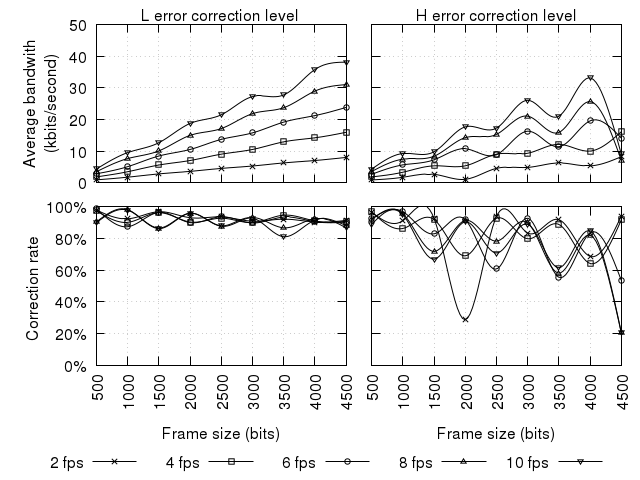
\includegraphics[width=\linewidth]{data1.png}
\caption{Bandwidth and decoding rate in the first experiment}
\label{img-exp1}
\end{center}
\end{figure}

As one can see, the recognition rates of higher correction level were lower than the ones of lower correction level, with all other parameters being equal. This can be explained by the fact that the same amount of data, carried inside a code with a higher correction level, has to display more modules. For example, according to Table \ref{tab:qr:sample-sizes}, the modules of a 2,000-bit, H-level code are as small as those of a 4,500-bit, L-level code. Smaller modules, in turn, yields increased difficulty in recognition by the camera. Therefore, a first conclusion one can draw is that, surprisingly, effective bandwidth seems to be improved by using a \emph{lower} level of error correction.

With the same data sizes and correction levels, the figure shows that the recognition rate decreases as the code rate increases. This can be explained by the fact that, in a higher code rate, the same code occupies fewer camera frames, and hence has fewer chances of being correctly decoded in one of the frames. Moreover, the probability that a code change occurs at the moment a frame is taken (resulting in a blurry image showing part of two different codes) is also increased. In the L level, the decrease is slight, but in the H level, the decrease is dramatic when the code size reaches 3,000 bits. As the data size increases, the recognition rate drops constantly and considerably.

These figures seem to indicate that the ideal configuration for level L is 4,500 bits and 10 fps, which yields an effective bandwidth of 39.0 kbps; for level H, 4,000 bits and 10 fps result in a bandwidth of 24.6 kbps.

\subsubsection{Double Display}

Considering that the camera might have missed several frames, we performed a second experiment in which every QR code is displayed twice within a small time window. Hence, instead of displaying each code once for $1/f$ second, each code was interleaved with neighbouring codes and displayed twice for $1/2f$ second each time. This results in the same total exposure time for each code, but increases the diversity in the images captured by the camera.

\begin{figure}[ht]
\begin{center}
\centering
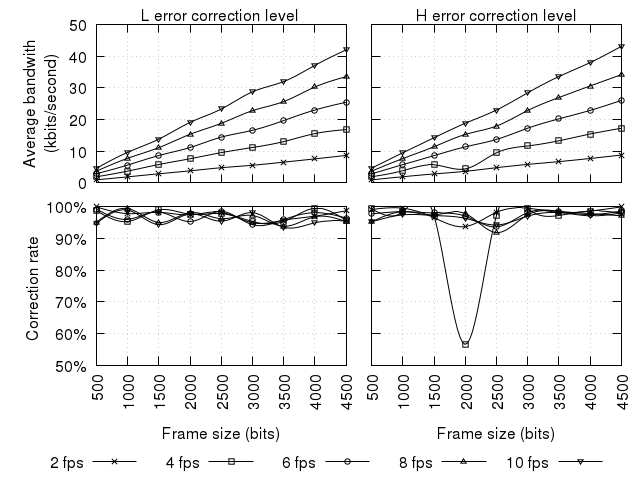
\includegraphics[width=\linewidth]{data2.png}
\caption{Bandwidth and decoding rate in the second experiment, where each code is displayed twice}
\label{img-exp2}
\end{center}
\end{figure}

The results are plotted in Figure \ref{img-exp2}. They show an increase in all recognition rates, which are now all higher than 90\%. This, in turn, increases the effective bandwidth; using the same settings as above, one can get a bandwidth of 43.0 kbps using level L, and 44.1 kbps using level H.

\subsubsection{Random Padding}

However, as we discussed earlier, not all QR codes are created equal; for the same resolution and error correction level, experimental results indicate that some codes seem to be more difficult to read than some others. Therefore, merely repeating the same image multiple times has no impact on that intrinsic ``hardness''. Our third experiment introduces yet another mechanism for boosting recognition rate.

This time, we tried to make the codes from the same input data different by appending, at the end of the data to be encoded, a small random string intended to change every time the code is to be displayed. Hence the same original data, if displayed twice, is prepended to a different random padding each time, yielding a slightly different array of bits. However, by virtue of the QR encoding schema, even a small change at the end of an array produces a completely different pattern of dots in the resulting QR code. Figure \ref{fig:qr:difcodes} shows an example of this phenomenon. Therefore, if a code is harder to read, the same data is also displayed in a largely different pattern of dots, increasing the odds of being properly picked up at least once.

\begin{figure}
\centering

\includegraphics[width=1in]{abcdefg.jpg}~
\includegraphics[width=1in]{abcdeff.jpg}
\caption{Examples of two codes with slightly different data, but widely different dot patterns. The code on the left contains the string ``abcdefg'', while the one on the right contains ``abcdeff''.}
\label{fig:qr:difcodes}
\end{figure}

Although the objective reason for some codes being harder to read is unknown and out of the focus of this chapter, experimental results seem to confirm this hypothesis. We performed a third experiment where every input data was displayed three times with different generated QR codes. The recognition rate is better than before when the code rate is lower than 10 fps, as shown in Figure \ref{img-exp3}. % the best bandwidth in L level is 44.9 kbps and in H level is 43.4 kbps.

\begin{figure}[ht]
\begin{center}
\centering
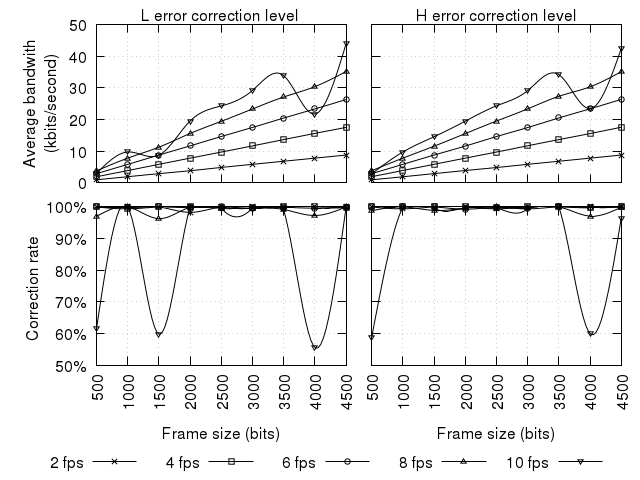
\includegraphics[width=\linewidth]{data3.png}
\caption{Third experiment: triple display and random padding}
\label{img-exp3}
\end{center}
\end{figure}

These results led us to experiment with higher code rates; we added 12 cps, 14 cps and 16 cps. The codes were displayed twice. As the Figure \ref{img-exp4} shows, the maximum effective bandwidth in the result is 65.5 kbps using level L, and 68.3 kbps in level H level, using 16 cps and 4,500-bit codes.

\begin{figure}[ht]
\begin{center}
\centering
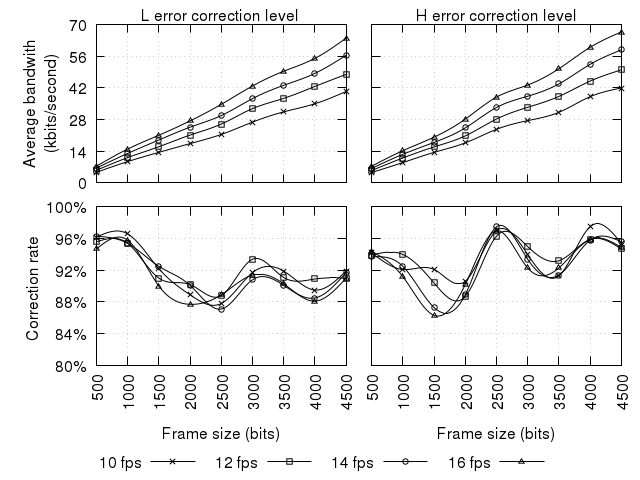
\includegraphics[width=\linewidth]{data4.png}
\caption{Fourth experiment: double display and higher code rates}
\label{img-exp4}
\end{center}
\end{figure}

\subsection{Partial Conclusions}

These initial experiments allow us to draw a few conclusions on the nature of a QR-based communication channel. First, although higher code rate and code size have a negative impact on the recognition ratio, the increased data that can be carried globally compensates for the higher error rate in terms of \emph{effective} bandwidth. Second, introducing repetition and varying the dot pattern for the same data increases the effective bandwidth; that is, showing two different codes for half the time is more effective than a single code for the same interval. Third, even for the smallest code sizes, the error rate of the channel is never zero, indicating that the channel is intrinsically lossy. 

From these findings, one can reasonably expect a QR code stream to provide a channel with an effective bandwidth of about 40 kbps, when displaying 10 4,000-bit codes per second using the random padding technique and L-level error correction. The decoding rate of the channel using these parameters should be of at least 95\%. Obviously, these findings apply to a fixed-camera setting. They do not take into account potential jitter, blurring or other effects that may occur in other contexts ---although an informal experiment described in Section \ref{subsub:swipe} tends to indicate the technology is relatively robust.

%% }}} --- Section

%% -----------------------
%% Section: le protocole
%% -----------------------
\section{A Protocol for One-Way, Lossy Communication Channels}\label{sec:qr:protocol} %% {{{

In this section, we propose an approach which uses continuous QR codes as a medium to achieve one-way data transmission.

\subsection{Design Goals}

In order to implement a communication channel, a specific protocol is essential; it should be well designed so that the data can be serialized and transferred without significant overhead. Besides, the protocol has to have the ability of splitting the to-be-transferred data into frames to generate the QR images. The result is BufferTannen, a Java software package dedicated to the serialization and transmission of structured data over limited communication channels.\footnote{\url{https://github.com/sylvainhalle/BufferTannen}} It provides a set of classes allowing the representation of structured data in a compact binary form. Contrarily to other systems, like Google's Protocol Buffers \footnote{\url{https://github.com/google/protobuf}}, defining new message types can be done at runtime and does not require compiling new classes to be used. Moreover, messages in BufferTannen cannot be encoded and decoded without prior knowledge of their structure. However, since messages do not contain information about their structure, they use much less space.

BufferTannen also defines a protocol allowing the transmission of messages.  Although any channel (TCP connection, etc.) can be used, BufferTannen was designed to operate on a channel with the following specifications, which are based on our initial experimental results:

\begin{itemize}
\item The channel is \emph{point-to-point}. The goal is to send information   directly from A to B; no addressing, routing, etc. is provided.
\item The channel is \emph{low-bandwidth} (that is, able to transmit a few hundred bytes at a time, possibly less than 10 times per second).
\item The channel is \emph{one-way}: typically, one side of the communication sends data that is to be picked up by some receiver. This entails that the receiver cannot acknowledge reception of data or ask the sender to transmit again, as in protocols like TCP.
\item The channel is \emph{lossy}. However, we assume that the channel provides a mechanism (such as some form of checksum) to detect when a piece of data is corrupted and discard it.
\item A receiver can start listening on the channel at any time, and be able to correctly receive messages from that point on. As such, the communication does not have a formal ``start'' that could be used, for example, to advertise parameters used for the exchange.
\end{itemize}

Therefore, the communication channel envisioned as the transmission medium for BufferTannen's messages can be likened in many ways to a slow broadcast signal, such as Hellschreiber \cite{hells}, slow-scan television \cite{slowtv}, Teletext \cite{teletext} or RBDS~\cite{rbds}.

BufferTannen's protocol aims at transmitting messages as reliably as possible under these conditions, while preserving the integrity of data and the ordering of messages. The low-bandwidth nature of the channel explains the emphasis on serializing messages in a compact binary form. Since the receiver cannot ask for any form of re-transmission, the protocol must provide for automatic re-transmissions of each message to maximize their chances of being picked up, while at the same time not confusing a re-transmission with a new message with identical content. Moreover, as the receiver can start listening at any moment, and that the schema of messages must be known in order to decode them, the schemas used in the communication must also be transmitted at periodic intervals.

\subsection{Schemas}
\setcounter{paragraph}{0}

The declaration of a data structure is called a \emph{schema}. Information can be represented in three different forms:

\begin{itemize}
\item Smallscii: A variable-length string of characters. Since BufferTannen is aimed towards limiting as much as possible the number of bits required to represent information, these strings are restricted to a subset of 63 ASCII characters (letters, digits and punctuation). Each character in a Smallscii string takes 6 bits, and each string ends with the 6-bit string \verb+000000+.

\item Integer: The only numerical type available in BufferTannen. When declared, integers are given a ``width'', i.e. the number of bits used to encode them. The width can be anything between 1 and 16 bits.

\item Enumeration: A list of predefined Smallscii constants. Enumerations can be used to further reduce the amount of space taken by a data element when its set of possible values is known in advance.
\end{itemize}

These basic building blocks can be used to write schemas by combining them using compound data structures:

\begin{itemize}
\item List: a variable-length sequence of elements, all of which must be of the same type (or schema). List elements are accessed by their index, starting
  with index 0.
\item FixedMap: a table that associates strings to values. The structure is fixed and the exact strings that can be used as keys must be declared. However, each key can be associated to a value of a different type.
\end{itemize}

These constructs can be mixed freely. The following represents the declaration of a complex message schema:

\begin{verbatim}
FixedMap {
  "title" : Smallscii,
  "price" : Integer(5),
  "chapters" : List [
     FixedMap {
       "name" : Smallscii,
       "length" : Integer(8),
       "type" : Enum {"normal", "appendix"}
     }
  ]
}
\end{verbatim}

The top-level structure for this message is a map (delimited by \verb+{+\dots\verb+}+). This map has three keys: \verb+title+, whose associated value is a Smallscii string, \verb+price+, whose associated value is a integer in the range 0-32 (i.e. 5 bits), and \verb+chapters+, whose value is not a primitive type, but is itself a list (delimited by \verb+[+...\verb+]+). Each element of this list is itself a map with three keys: a string \verb+name+, an integer \verb+length+, and \verb+type+ whose possible values are \verb+normal+ or \verb+appendix+.

Schemas can be represented in a compact and unequivocal binary representation as follows.

\paragraph{Integer} The declaration of an integer is encoded as the following sequence of bits:
%
\begin{verbatim}
ttt wwwww ddddd s
\end{verbatim}

The sequence \verb+ttt+ represents the element type, encoded on 3 bits. An integer contains the decimal value 6. The sequence of \verb+w+ indicates the integer's width in bits. The width itself is encoded over 5 bits. The sequence of \verb+d+ indicates the integer's width, in bits, when expressed as a delta value, i.e.\ as the difference with respect to an integer from a previous message. The width itself is encoded over 5 bits. The single bit \verb+s+ is the sign flag. If set to 0, the integer is unsigned; if set to 1, the integer is signed. Note that integers expressed as delta values are always encoded as signed integers; hence this flag only applies to integers occurring as full values.

\paragraph{Smallscii string} The declaration of a Smallscii string is simply coded as three bits representing the element type; a string contains the decimal value 2.

\paragraph{Enumeration} An enumeration must provide the list of all possible values it can take. It is formally represented as:
%
\begin{verbatim}
ttt llll [ssssss ssssss ... 000000 ...
 ssssss ssssss ... 000000]
\end{verbatim}

The element type is the decimal value 1, and the sequence \verb+llll+ is the number of elements in the enumeration, encoded on 4 bits. What follows is a concatenation of Smallscii strings defining the possible values for the enumeration. Each character is encoded on 6 bits, and the end of a string is signalled by the 6-bit sequence \verb+000000+.

\paragraph{List} The declaration of a list is as follows:
%
\begin{verbatim}
ttt llllllll ...
\end{verbatim}

The element type is the decimal value 3; the 8-bit sequence \verb+llllllll+ defines the maximum number of elements in the list. What follows is the declaration of the element type for elements of that list.

\paragraph{Fixed Map} The last element type is the fixed map, declared as follows:
%
\begin{verbatim}
ttt [ssssss ssssss ... 000000 ddd...]
\end{verbatim}

The element type is the decimal value 4; what follows is a Smallscii string defining the name of a key, followed by the declaration of the element type for that key; this is repeated for as many keys the map declares.

\subsection{Messages}
\setcounter{paragraph}{0}

A \emph{message} is an instance of a schema. For example, the following is a possible message abiding by the previous schema:

\begin{verbatim}
{
  "title" : "hello world",
  "price" : 21,
  "chapters" : [
    {
      "name" : "chapter 1",
      "length" : 3,
      "type" : "normal"
    },
    {
      "name" : "chapter 2",
      "length" : 7,
      "type" : "normal"
    },
    {
      "name" : "conclusion",
      "length" : 2,
      "type" : "appendix"
    }
  ]
}
\end{verbatim}

The reader familiar with JSON or similar notations will notice strong similarities between BufferTannen and these languages. As a matter of fact, elements of a message can be queried using a syntax similar to JavaScript. For example, assuming that \verb+m+ is an object representing the above message, fetching the length of the second chapter would be written as the expression:

\begin{verbatim}
m[chapters][1][length]
\end{verbatim}

This fetches the \verb+chapters+ value in the top-level structure (a list), then the second element of that list (index 1), and then the \verb+length+ value of the corresponding map element.

As with schemas, messages can be represented in a compact binary form.

\paragraph{Smallscii string} Strings are represented as a sequence of 6-bit characters, terminated by the end of string delimiter \verb+000000+.

\paragraph{Integer} Numbers are represented by the sequence of bits that encodes their value, without any terminating sequence: the number of bits to read is dictated by the size of the integer, as specified by the corresponding schema element. If the integer is signed, the first bit represents the sign (0 = positive, 1 = negative) and the remainder of the sequence represents the absolute value. %(Yes, this means that there are two ways of encoding 0 in a signed integer, either as -0 or as +0. Both will correctly be decoded as 0.)

\paragraph{Enumeration} An enumeration is simply made of the sequence bits corresponding to the appropriate value. Again, the number of bits to read is dictated by the size of the enumeration, as specified in the schema of the message to read. For example, if the enumeration defines 4 values, then 2 bits will be read. The numerical value $i$ corresponds to the $i$-th string declared in the enumeration.

\paragraph{List} A list begins by 8 bits recording the number of elements in the list. The remainder of the list is the concatenation of the binary representation of each list element. Since the type of each element and the number of such elements to read are both known, no delimiter is required between each element or at the end of the list.

\paragraph{Fixed Map} The contents of a fixed map is simply the concatenation of the binary representation of each map value. The key to which each value is associated, and the value type to read, are specified in the schema of the message to read, and are expected to appear exactly in the order they were declared. This spares us from repeating the map's keys in each message.

\subsection{Reading and Writing Messages}

In BufferTannen, both schemas and instances of schemas are represented by the same object, called \verb+SchemaElement+. An empty SchemaElement must first be instantiated using some schema; this can be done by either:

\begin{itemize}
\item Reading a character string formatted as above; or

\item Reading a binary string containing an encoding of the schema. As a matter of fact, in BufferTannen both messages \emph{and} schemas can be transmitted in binary form over a communication channel, and a method is provided to export the schema of some message into a sequence of bits.
\end{itemize}

Once an empty SchemaElement is obtained, it can be filled with data, again in two ways:

\begin{itemize}
\item By reading a character string formatted as above; or

\item By reading a binary string containing an encoding of the data.
\end{itemize}

Similar methods exist to operate in the opposite way, and to \emph{write} a message's schema or data contents either as a character string or as a binary string. This way, messages and schemas can be freely encoded/decoded using human-readable text strings or compact binary strings.

As one can see, for a message to be read or written, it is necessary first to instantiate an object with a schema. As a matter of fact, trying to decode a stream of data without first advertising the underlying schema will cause an error, even if the stream contains properly formatted data. Similarly, trying to read data that uses some schema with an object instantiated with another schema will also cause an error. In other words, no data can be read or written without knowledge of the proper schema to use.

This might seem restrictive, but it allows BufferTannen to heavily optimize the binary representation of messages. In the absence of a known schema, each message would require to carry, in addition to its actual data, information about its own structure. %Since a reader receiving a sequence of bits would not know in advance how to read it, special sequences would need to be added to notify the reader that what follows is a map with some number of keys, and then in turn each value for each key would also need to declare the structure of its own type, and so on.
%
Practically speaking, this amounts to repeating within each message the description of its schema, interspersed through the message data. On the contrary, if the schema is known, all this signaling information can be discarded: when receiving a sequence of bits, a reader that possesses the schema knows exactly how many bits to read, what data this represents and where to place it in the message structure being populated. This entails, however, that a receiver that does not know the schema to apply has no clue whatsoever on how to process a binary string.

To illustrate the interest of BufferTannen as a message encoding scheme, we consider the example of transmitting events from a video game to an external monitor.

\subsection{Segments}
\setcounter{paragraph}{0}

Messages and schemas are encapsulated into a structure called a \emph{segment}. A segment can be of four types:

\paragraph{Message segments} contain the binary representation of a message, along with a sequential number (used to preserve the ordering of messages received), as well as the number referring to the schema that must be used to decode the message. A message segment consists of a header structured as follows:

\begin{verbatim}
tt nnnnnnnnnnnn wwwwwwwwwwww ssss ...
\end{verbatim}

The header starts with two bits describing the type of the segment; a message segment contains the decimal value 1. The \verb+n+ and \verb+w+ sections describe the segment's sequential number and total length, both encoded on 12 bits. The four \verb+s+ bits provide the schema number in the schema bank that should be used to read this segment. The remainder of the segment is comprised of a map, list, Smallscii string or number, whose binary representation was described above.

\paragraph{Schema segments} contain the binary representation of a schema, which is associated to a number. Multiple schemas can be used in the same communication, hence creating a bank of schemas identified by their number. A schema segment consists of a header structured as follows:

\begin{verbatim}
tt nnnnnnnnnnnn ssss ...
\end{verbatim}

The header starts with two bits describing the type of the segment; a schema segment contains the decimal value 2. The \verb+n+ section describes the segment's sequential number, and the \verb+s+ section gives the the schema number in the schema bank this segment should be assigned to. The remainder of the segment is comprised of a binary string describing the schema, whose representation was described above.

\paragraph{Blob segments} are intended to carry raw binary data over the BufferTannen protocol.

\paragraph{Delta segments} contain the binary representation of a message, expressed as the difference (``delta'') between that message and a previous one used as a reference. Delta segments are used to further compress the representation of a message, in the case where messages don't change much over an interval of time.

\begin{verbatim}
tt nnnnnnnnnnnn wwwwwwwwwwww rrrrrrrrrrrr...
\end{verbatim}

The header starts with two bits describing the type of the segment; a delta segment contains the decimal value 1. The \verb+n+ and \verb+w+ sections describe the segment's sequential number and total length, both encoded on 12 bits. The \verb+r+ section gives the sequential number of another segment, relative to which the delta of the current segment are expressed. What follows is a binary string that describes the ``difference'' one must compute with respect to that segment to obtain the contents of the current one.

The computation of the delta is performed recursively on each element of the two messages to compare in the order they occur. It is defined for each element type as follows.

\begin{itemize}
\item Smallscii strings: if the corresponding strings are identical, emit the single bit \verb+0+. Otherwise, emit the bit \verb+1+ followed by the Smallscii string of the target message.
%
\item Integers: if the corresponding numbers are identical, emit the single bit \verb+0+. Otherwise, emit the bit \verb+1+ followed by the difference between the source and the target integer.
%
\item Enumerations: if the corresponding value of the enumerated type is the same, emit the single bit \verb+0+. Otherwise, emit the bit \verb+1+ followed by the integer value corresponding to the index of the value in the target message.
%
\item Lists: if both lists have the same elements in the same order, emit the single bit \verb+0+. Otherwise, emit the bit \verb+1+ followed by the binary representation of the target list.
%
\item Maps: recursively apply the previous rules for each key of the map.
\end{itemize}

One can see that delta segments apply only a coarse form of comparison. For example, no attempt is made to detect whether two lists differ by the addition or deletion of an element; the contents of the list is retransmitted in full whenever it is not identical to the original. Nevertheless, this technique allows substantial savings whenever a part of a data structure remains identical from one message to the next.

\subsection{Frames}
\setcounter{paragraph}{0}

The communication channel sends binary data in units called \emph{frames}. A frame is simply a set of concatenated segments in binary form, preceded by a header containing the version number of the protocol (currently ``1'') and the length (in bits) of the frame's content. Formally, the binary structure of a frame is as follows:

\begin{verbatim}
vvvv nnnnnnnnnnnnnn ffff... ffff...
\end{verbatim}

The \verb+v+ section consists of the 4-bit protocol version number, followed by 14 bits indicating the total length (in bits) of the frame. Each segment is appended directly to this 18-bit header. As each segment's header contains its own length, no further marshaling is required to correctly decode segment data.

When many segments are awaiting to be transmitted, the protocol tries to fit as many segments as possible (in sequential order) within the maximum size of a frame before sending it. This maximum size can be modified to fit the specifics of the communication channel that is being used. In the current incarnation of the protocol, segments cannot be fragmented across multiple frames. Hence a segment cannot exceed the maximum size of a frame.

Each frame is then converted into a QR code, with its binary content Base64-encoded as the code's text. This QR code can then be read at the receiving site, converted into a binary sequence, and parsed back into frames, segments and messages by applying the reverse transformations.

\subsection{Streaming Modes}
\setcounter{paragraph}{0}

BufferTannen is designed with two sending modes, respectively called ``Lake'' mode and ``Stream'' mode.

Lake mode is intended for the sending of a finite piece of data, such as a file, or a sequence of BufferTannen messages whose complete contents are known in advance. The data to be sent is divided into a finite set of segments, and the whole sequence of segments is repeatedly emitted through QR codes. If any frames are missed or incorrectly decoded, the infinite repetition of all segments makes possible to catch the missing data at the next loop. Ultimately, decoding errors may entail that the data needs to be read for more than one loop before it is completely received.

The use of Lake mode can be detected by frames carrying a non-zero value to their ``total segments'' header field. Hence a receiver that starts reading at any point through the sequence of frames knows how many segments in total are to be received, and the relative position of each segment in the data to be reconstructed. This makes Lake mode a relatively slow, but very robust optical data transmission scheme.

In Stream mode, the data is continuously read into segments which then form a stream of frames, and the frames are immediately sent. The reading process stops only when there is no more data to read. The frames already sent are removed from the memory, so there is no way to resend the data for several times. However, for the sake of the data consistency, we made a buffer for the clones of the sent frames, and after having sent a specific amount frames fetched from the original data, the frames in the buffer are resent again and then removed from the buffer. Therefore, Stream mode is intended to send realtime data, typically where where the data loss is acceptable and the consistency can be slightly sacrificed (e.g.\ audio or video).

\begin{figure*}
\centering
\begin{verbatim}
--------------------------------------------------------------------------
Sending mode:        lake
Buffer state:        [||>       ||:.::||:|||] 59% (130/219)
Progress:            0408/0000 (13.8 sec @30 fps)
Link quality:        22/30 [*******   ] (73%)  Global:   339/454 (74%)
Data stream index:   0
Resource ident.:     myfile.jpg
Processing rate:     35 ms/frame (27 fps)
--------------------------------------------------------------------------
\end{verbatim}
\caption{Part of the text interface of the QR code receiver operating in Lake mode}
\label{fig:qr:lake-gui}
\end{figure*}

Figure \ref{fig:qr:lake-gui} shows a portion of the text interface of our QR code receiver implementation. The interface shows that the frames being received are in Lake mode. The buffer state field indicates the progress of the reception. In the example, it shows that 130 out of 219 segments have been correctly received; the text bar at the left indicates to what portions of the total sequence these segments correspond. A section of the sequence that has not been received at all is indicated by a blank space; increasingly full portions of the sequence are represented respectively by the symbols \verb+.+, \verb+.+ and \verb+|+. The \verb+>+ symbol indicates the relative position of the last segment that was correctly read.

The ``Link quality'' field gives a realtime indication of the decoding rate. It shows that 22 of the last 30 images captured by the camera were correctly decoded, and that globally, 339 images were decoded out of 454 captured. The resource identifier and data stream index, carried by each frame, is also displayed.

\subsection{Experimental Results}
\setcounter{paragraph}{0}

The experiments of Section \ref{sec:qr:experiments} confirmed our intuition that optical code streams are an inherently unreliable and low-bandwidth communication channel. The compactness of the BufferTannen protocol can be motivated by an example from runtime verification. A particular video game, called Pingus, was instrumented to produce events containing the state of every character in the game. The schema for these events is shown in Figure \ref{fig:qr:pingus-schema}.

\subsubsection{File Transfer}

\begin{figure}
\centering
\begin{verbatim}
FixedMap {
  "pingus" : List [
    FixedMap [
      "id" : Integer(6),
      "x" : Integer(10),
      "y" : Integer(10),
      "velocity-x" : Integer(4),
      "velocity-y" : Integer(4),
      "state" : Enum {"floater",
         "basher", "builder",
         "athlete", "normal"}
    ]
  ]
}
\end{verbatim}
\caption{The schema of events produced by an instrumented video game.}
\label{fig:qr:pingus-schema}
\end{figure}

An event typically contains data for 50 characters, hence the map structure is repeated that many times. Sending such an event in clear-text format, without any whitespace, takes roughly 3,750 bytes. At a rate of 30 events per second, it takes 879 kbps of bandwidth to transmit the event stream. The same event in BufferTannen takes 1,856 \emph{bits}, or 232 bytes. This divides by more than 16 the bandwidth requirements for sending a stream of such events, yielding a bandwidth of 54 kbps.\footnote{Sending the same character string into Gzip shrinks it down to 716 bytes, which makes standard compression a less appealing alternative in that context.} From that point on, delta segments can be used to further reduce the stream's bandwidth, and transmit the remaining events using slightly more than 100 bytes each, consuming a bandwidth of approximately 24 kbps. Our previous experiments show that this is within the range of what one can reasonably expect to transmit using QR codes.

We then tested the ability of the BufferTannen protocol to mitigate these defects, through its use of repetition and its compact binary representation.\footnote{A video of BufferTannen in action is available online: \url{https://www.youtube.com/watch?v=GSL0md0TlY8}}

We chose to encode data into 4,000-bit codes, which, after the encapsulation of BufferTannen, amounts to a QR code of about 5,800 bits. With the combination of 5800 bits and L correction level, according to Table \ref{tab:qr:sample-sizes}, the symbol size is about 93 $\times$ 93 which is between the combinations of 3,500-bit, H-level and 4,000-bit, H-level. From the result of the last experiment, the combinations of 4,000-bit, H level and any sample fps has more than 95\% correction rate which is reliable. Secondly, the code rates were 4, 6, 8, 10, 12 fps. According to the last experiment, this configuration is reliable and supposed to be able to supply 23.2--69.6 kbps, and 16.0--48.0 kbps of bandwidth, respectively.
%
In the consideration of the practical application, we chose to transfer a sample file of which the size is 37,656 bytes, and we performed each experiment 20 times.

The result of the Lake mode experiment in Figure \ref{img-explake} shows that the best fps value is 10, and in this case the sample file needed to be transferred on average 2.4 times to make sure that the receiver could get all the frames. The average spent time is 17.27 seconds, from which the bandwidth is about 17.0 kbps.

\begin{figure}[ht]
\begin{center}
\centering
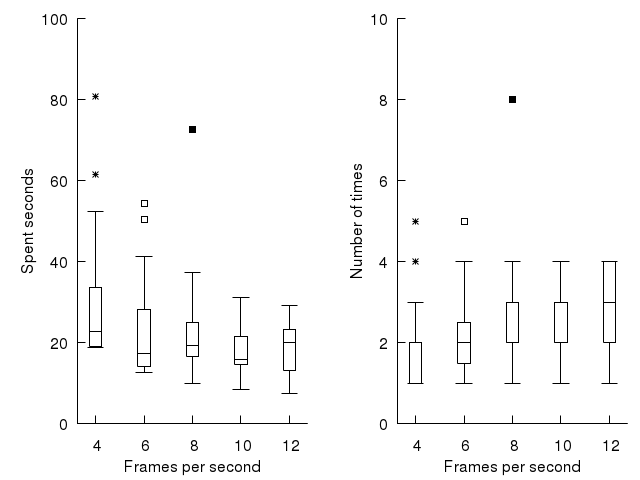
\includegraphics[width=\linewidth]{lake.png}
\caption{Time to send data in Lake mode}
\label{img-explake}
\end{center}
\end{figure}

In Stream mode, the percentage of received codes is important. In the experiment, according to Figure \ref{img-expstream}, the average completion ratios of all configurations are over 99\%, and the configuration of 12 fps needs approximately 13.11 seconds to send all frames with a data streaming channel of 22.4 kbps.

\begin{figure}[ht]
\begin{center}
\centering
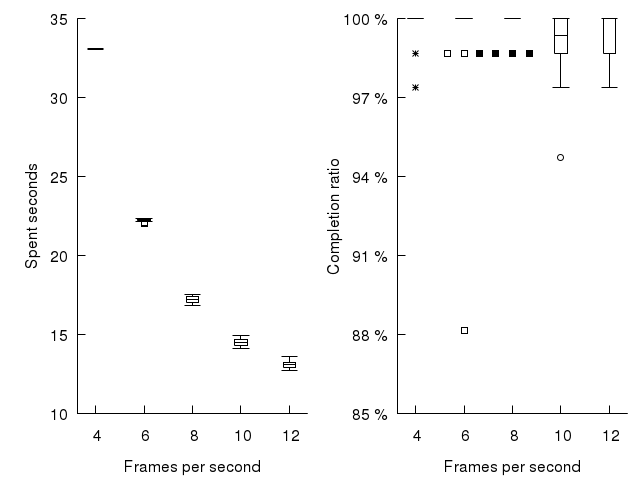
\includegraphics[width=\linewidth]{stream.png}
\caption{Time to send data in Stream mode}
\label{img-expstream}
\end{center}
\end{figure}

\subsubsection{Paper Swiping}\label{subsub:swipe}

The ability to send streams of data in Lake mode can also be used to supplement QR codes' inherently limited capacity. When displaying a printed code on a piece of paper, large amounts of data can be carried only through increasing the code's resolution; however, resolution can only be increased up to a certain, predefined limit.\footnote{4,296 alpha-numeric characters, or 3,222 bytes assuming Base-64 encoding.} Moreover, for higher resolutions, the code may become hard to read using entry-level, low-resolution cameras. Therefore, it is safe to assume that, using existing QR code technology, no more than 3,000 bytes of data can be transferred using a QR code.

This limitation can be overcome by the use of the BufferTannen protocol. Although no code larger than roughly 4,000 bytes can be created, multiple such codes can be lined on a piece of paper. Each such code can be formatted to contain a single frame of data sent by the BufferTannen protocol in Lake Mode. It suffices for a user to swipe the camera over these multiple codes; by virtue of Lake Mode, the order in which the codes are scanned is irrelevant, and the complete piece of data can be correctly reconstructed from the individual frames. It is therefore possible to transmit theoretically unlimited amounts of data, while using codes of a lower resolution (this lower resolution being compensated by the presence of more than one code).

To verify this claim, we printed on a piece of paper the contents of a 37 kb file as a sequence of QR codes, processed as frames through BufferTannen in Lake Mode. We then hovered the camera over that sheet of paper at arm's length (see Figure \ref{fig:qr:paper-swipe}). The software's user interface displayed in real time the number of frames remaining to be decoded and their location in the complete stream, giving indications to the user as to which codes to swipe over. It shall be noted that the camera operated in ``film'' mode, and not in ``snapshot'' mode. In other words, images were continuously captured by the camera as it was being moved over the sheet; the user did not need to point and click at each individual QR code (which would be fastidious).

\begin{figure}
\centering
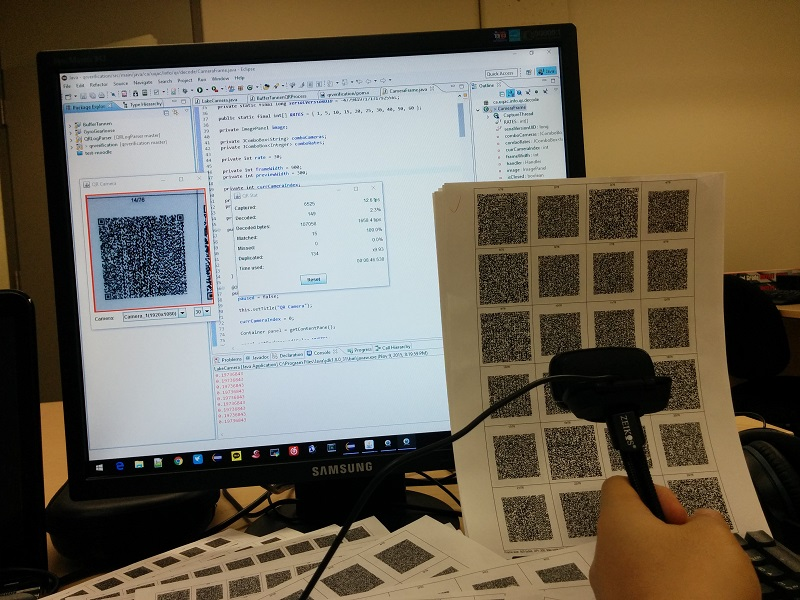
\includegraphics[width=\linewidth]{swipe.jpg}
\caption{Swiping the camera over a set of QR codes to reconstruct the contents of a larger file.}
\label{fig:qr:paper-swipe}
\end{figure}

The error correction level chosen was L and the sizes of raw data per code that we tested were 500, 750, 1,000, 1,250, 1,500, 1,750, and 2,000 bytes. With 500 bytes there were 76 codes while with 2,000 bytes there were only 19. After being encapsulated by BufferTannen protocol, the final sizes of data used to generate the QR codes became correspondingly 723, 1,055, 1,391, 1,724, 2,054, 2,389, and 2,722 bytes. The codes were printed at 300 dpi and 600 dpi on standard office paper, and we programmed to give each edge of every code 500 dots in the paper.

At 300 dpi, the codes of size ranging from 500 to 1,250 bytes were all decoded successfully and smoothly. However, when the size reaches 1,500 bytes, the decoding becomes more problematic. For some codes, we had to retry for several times by sticking the camera near the paper for a few seconds, yet among the total 31 codes, three remained impossible to decode at all. In the case of codes of 1,750 and 2,000 bytes, none of the codes could be decoded. This can be explained by the fact that higher density codes entail that each module of the code is smaller and hence harder to capture. For example, the edge of a 500-bytes and L-level code is about 77 modules, so each module can have approximately 6 dots in the paper, while the edge of a 2000-bytes, L-level code is 149 modules, so each module amounts to only 3 printed dots.

At 600 dpi, none of the codes could be decoded, no matter how many bytes they carried. The reason is that the codes printed at 600 dpi are too small and the camera has to approach very closely to the paper, but the captured images were all blurred and out of focus. It therefore seems that codes printed at 600 dpi are beyond the ability of a standard web camera.

Nevertheless, this experiment demonstrates the viability of the concept of hovering a camera across an array of QR codes. Our empirical findings indicate that a stream of data can be split into a set of QR codes of about 1,000 bytes each, the contents of which correspond to individual frames of the BufferTannen protocol containing the data to be transmitted. Swiping the camera over this set of codes, in no particular order, is sufficient to reconstruct on the device side the complete data contents.

%% }}} --- Section

%% -----------------------
%% Section: Conclusion
%% -----------------------
\section{Conclusion}\label{sec:qr:conclusion} %% {{{

In this chapter, we presented a solution for a one-way communication channel based on QR codes, and performed experiments to measure its performance. We first experimentally tested the characteristics of a QR data stream under various conditions, and extracted the parameters maximizing the effective bandwidth of the channel. However, since that channel is inherently error-prone and low-bandwidth, we then introduced BufferTannen, a protocol designed especially for this kind of channel. BufferTannen takes care of splitting, marshaling, and to some extend compressing the data to transmit in order to maximize the efficiency of the QR code stream. The feasibility of this approach was then empirically observed through a new set of experiments.

Within the limits of the protocol and of the communication channel, the presented results can be put to good use in a variety of situations. In limited environments where the use of radio signal or cables is forbidden or difficult, our approach can provide an easy way to communicate between peers, either as an emergency backup or as a primary means. Furthermore, the evolution of the quality of both display and image capture devices makes it possible to foresee increased transmission rates in the future. %as the performance of common devices keeps increasing, the symbols containing more data, or even some more complicated symbol formats can be brought into concern.
Finally, the aforementioned techniques could be turned into a bidirectional communication link in the case of endpoints equipped with both a camera and a display. In such a case, acknowledgments of correctly decoded images could be exchanged, which in turn would allow resending data on demand and increase the effective bandwidth.

%% }}} --- Section
%!TEX root = these.tex

\chapter{Offline Evaluation of LTL Formulæ with Bitmap Manipulations}

This chapter represents a modified version of a paper which is written by K. Xie and S. Hallé and still under review for publication in the proceedings of the International Conference: Runtime Verification 2016 (RV'16) in Madrid, Spain in 2016.

%% ------------------
%% Section: intro
%% ------------------
\section{Introduction}\label{sec:bm:intro} %% {{{

\emph{Temporal logic} \cite{huth2004} is a logistic system which uses rules and symbols to describe and reason about the change of a system's state in terms of time. It is based on the idea that one state may not be constantly true or false as time goes. \emph{Linear Temporal Logic (LTL)} \citep{pnueli97} is a temporal logic, and as its name entails, \emph{LTL} can denote only one sequence of states and for each state there is only one future state.

A \emph{bitmap}, also known as a bit array or bitset, is a compact data structure storing a sequence of binary values. As will be shown in Section \ref{sec:bm:compression}, it can be used to express a set of numbers, or an array where each bit represents a 2-valued option. Bitmaps present several advantages as a data structure: they can concisely represent information, and provide very efficient functions to manipulate them, taking advantage of the fact that multiple bits can be processed in parallel in a single CPU instruction.

In this paper, we explore the idea of using bitmap manipulations for the offline evaluation of LTL formul\ae{} on an event log. For this purpose, in Section \ref{sec:bm:ltlbitmap}, we introduce a solution which, for a given event trace $\sigma$ and an LTL formula $\varphi$, first converts each ground term into as many bitmaps; intuitively, the bitmap for atomic proposition $p$ describes which events of $\sigma$ satisfy $p$. Algorithms are then detailed for each LTL operator, taking bitmaps as their input and returning a bitmap as their output. The recursive application of these algorithms can be used to evaluate any LTL formula.

This solution presents several advantages. First, the use of bitmaps can be seen as a form of \emph{indexing} (in the database sense of the term) of a trace's content. Rather than being an online algorithm merely reading a pre-recorded trace, our solution exploits the fact that the trace is completely known in advance, and makes extensive use of this index to jump to specific locations in the trace to speed up its process. Second, a bitmap having consecutive 0s or 1s can be compressed, which reduces the space cost and speeds up the execution of many operations even further \citep{lemire2014}.

To this end, Section \ref{sec:bm:experiments} describes an experimental setup used to test our solution. It reveals that, that, for complex LTL formul\ae{} containing close to 20 temporal operators and connectives, large event traces can be evaluated at a throughput ranging in the tens of millions of events per second. These experiments show that the bitmaps are a compact and fast data structure, and are particularly appropriate for the kind of manipulations required for offline monitoring.

%% }}} --- Section

%% ------------------
%% Section: bitmap compression
%% ------------------
\section{Bitmaps and Compression}\label{sec:bm:compression} %% {{{

A bitmap (or bitset) is a binary array that we can view as an efficient and compact representation of an integer set. Given a bitmap of $n$ bits, the $i$-th bit is set to 1 if the $i$-th integer in the range $[0, n-1]$ exists in the set.

It was recognized early on that bitmaps could provide efficient ways of manipulating these sets, by virtue of their binary representation. For example, union and intersection between sets of integers can be computed using bitwise operations (OR, AND) on their corresponding bitmaps; in turn, such bitwise operations can be performed very quickly by microprocessors, and even in a single CPU operation for 32 or 64-bit wide chunks, depending on the architecture

Furthermore, a bitmap can be used to map $n$ chunks of data to $n$ bits. If the size of each chunk is greater than 1, the bitmap can greatly reduce the size of the storage. In addition, with its capacity of exploiting bit-level parallelism in hardware, standard operations on bitmaps can be very efficient. Unsurprisingly, bitmaps have been used in a lot of applications where the space or speed requirements are essential, sucha as information retrieval \cite{Chan:1998:BID:276305.276336}, databases \cite{burdick2001mafia}, and data mining \cite{Ayres:2002:SPM:775047.775109,Uno:2005:LVC:1133905.1133916}.

A bitmap with low fraction of bits set to value 1 can be considered \emph{sparse} \cite{lemire2014}. Such a sparse bitmap, stored as is, is a waste of both time and especially space. Consequently, many algorithms have been developed to \emph{compress} these bitmaps; most of them there are based on the Run-Length Encoding (RLE) model derived from the BBC compression scheme \cite{antoshenkov1995byte}. In the following, we briefly describe a few of these techniques. In particular, we detail the WAH \cite{wu2006optimizing}, Concise \cite{colantonio2010} and EWAH\cite{lemire2010} algorithms, because they have well-implemented open source libraries in Java that we will evaluate experimentally later in this paper.

\subsection{WAH}

WAH \citep{wu2006optimizing} divides a bitmap of $n$ bits into $\lceil \frac{n}{w-1}\rceil$ words of $w -1$ bits, where $w$ is a convenient word length (for example, 32). WAH distinguishes between two types of words: words made of just $w-1$ ones ($11\dots 1$) or just $w-1$ zeros ($00\dots 0$), are \emph{fill words}, whereas words containing a mix of zeros and ones are \emph{literal words}. Literal words are stored using $w$ bits: the most significant bit is set to zero and the remaining bits store the heterogeneous $w-1$ bits. Sequences of homogeneous fill words (all ones or all zeros) are also stored using w bits: the most significant bit is set to 1, the second most significant bit indicates the bit value of the homogeneous block sequence, while the remaining $w-2$ bits store the run length of the homogeneous block sequence.

\subsection{Concise}

Concise \citep{colantonio2010} is a bitmap compression algorithm based on WAH. Comparing with WAH, for which the run length is $w-2$ bits, Concise uses $w - 2 - \lceil \log_2 w \rceil$ for the run length and $\lceil \log_2 w \rceil$ bits to store an integer value indicating to flip a bit of a single word of $w-1$ bits. This feature can improve the compression ratio in the worst case.

\subsection{EWAH}

EWAH \cite{lemire2010} is also a variant of WAH but it does not use its first bit to indicate the type of the word like WAH and Concise. EWAH rather defines a $w$-bits marker word. The most significant $w/2$ bits of the word are used to store the number of the following fill words (all ones or all zeros) and the rest $w/2$ bits encodes the number of \emph{dirty words}. These words are exactly like the literal words of WAH, but utilize all $w$ bits. 

With respect to WAH and Concise, the structure used for EWAH makes it difficult to recognize a single word in the sequence as a marker word or a dirty word without reading the sequence from the beginning. Hence, apart from exceptional situations, a reverse enumeration of the bits in the sequence is nearly impossible.

\subsection{Roaring}

In all the previous models, fast random access to the bits in an arbitrary sequence is relatively difficult. At the very least, the word that contains the bit to read must be identified, and the position of this word in the stream requires a knowledge of how many literal or fill words are present before. Besides the RLE-model algorithms, there exist other bitmap compression models that support fast random access similar to uncompressed bitmaps. One of them is called ``Roaring bitmap'' \cite{lemire2015}, which we shall briefly describe.

Roaring bitmap has a compact and efficient two-level indexing data structure that splits 32-bit indexes into chunks, each of which stores the 16 most significant bits of a 32-bit integer and points to a specialized container storing the 16 least significant bits. There are two types of containers: a sorted 16-bit integer array for \emph{sparse} chunks, which store at most 4,096 integers, and a bitmap for \emph{dense} chunks that stores $2^{16}$ integers. This hybrid data structure allows fast random access whereas all RLE-model algorithms mentioned cannot because of the characteristics mentioned earlier.

%The time complexities of the LTL operators with \emph{Roaring bitmap} are $O(n)$ because we cannot skip certain bits when enumerating the bitmap.

\subsection{Discussion}

The RLE-model algorithms share some common features and also have their own characteristics. First, all of them have two different kinds of words, one of which is to store the raw uncompressed word (literal word) and the other is compressed word (sequence word) having a bit and a number. The number represents the number of consecutive words which are full of 0s or 1s determined by the bit.

We use $wlen$ to represent the number of bits in a word, $ulen$ the number of available in a literal word and $wcap$ the maximum number of bits stored in a sequence word. Table \ref{tbl:bm:bmparms} lists the parameters of the three RLE-model algorithms.

\begin{table}[h]
\centering
\begin{tabular}{|c|c|c|c|}
\hline
& ulen & wlen & wcap \\
\hline
WAH & 31 bits & 32 bits & $2^{30} - 1$ \\
\hline
Concise & 31 bits & 32 bits & $2^{25} - 1$ \\
\hline
EWAH & 32 or 64 bits & 32 or 64 bits & $2^{16} - 1 \text{ or } 2^{32} - 1$ \\
\hline
\end{tabular}
\caption{Parameters of RLE-model algorithms}
\label{tbl:bm:bmparms}
\end{table}

Considering that a $n$-bits bitmap has $m$ sequences of consecutive (0...1...) bits:
\begin{align*}
& c^1_0c^0_1c^1_1c^0_1c^1_2c^0_2...c^1_{m - 1}c^0_{m - 1}, c^i_j \text{ is the number of } \\
& \text{consecutive } i \text{ bits and } i \in (0, 1),\, 0 \leq j \leq m.  
\end{align*}

Then the number of total bits, i.e. the size of the uncompressed bitmap is:
\begin{align*}
& total\_bits = \sum_{j = 0}^{m - 1} \sum_{i = 0}^1 c^i_j = \sum_{j = 0}^{m - 1} \sum_{i = 0}^1 l^i_j + s^i_j, \\
& l^i_j = c^i_j \text{ mod } ulen, s^i_j = c^i_j - l^i_j
\end{align*}

If exists a positive integer $slen$, $\forall c^i_j = slen$, then
\begin{align}
m = n \div (2 \times slen) \label{eq:seqnum}
\end{align}

When $1 \leq slen < wlen$, then $\forall l^i_j > 0, \forall s^i_j = 0$, which is considered the worst case, the size of the compressed bitmap is:
\begin{align*}
compressed\_bits = \lceil \frac{total\_bits}{ulen} \rceil \times wlen 
\end{align*}

None of the three RLE-model algorithms can well compress this kind of bitmap. Both \emph{WAH} and \emph{Concise} waste one bit for the type identification and \emph{EWAH} seems to cost the least for its $ulen = wlen$ but its actual size should be a little more than $total\_bits$ because some empty sequence word is needed to store the number of the literal words.

Furthermore, when $wlen \leq slen$, then $\forall s^i_j > 0$, the sequence can be well compressed with any RLE-model algorithm. Suppose $\forall l^i_j > 0$, the size of the compressed bitmap is:
\begin{align*}
compressed\_bits = &\sum_{j = 0}^{m - 1} \sum_{i = 0}^1 \lceil \frac{slen}{wcap} \rceil \times wlen + wlen \\
= & 2 \times m \times wlen \times (1 + \lceil \frac{slen}{wcap} \rceil)
\end{align*}

From this discussion, we can see that $slen$, i.e. the number of consecutive 1 or 0 bits in a sequence, is a crucial argument and is able to decide the compression rate of a RLE bitmap compression algorithm. Some optimization like Concise is merely to try to improve the performance of the worst case.

%% }}} --- Section

%% ------------------
%% Section: algos
%% ------------------
\section{Evaluating LTL formul\ae{} with Bitmap}\label{sec:bm:ltlbitmap} %% {{{

Since bitmaps have been shown to be very efficient for storing manipulating encoded sets of integers, in this section we describe a technique for evaluating arbitrary formul\ae{} expressed in Linear Temporal Logic on a given trace of events through bitmap manipulations.

\subsection{Preliminaries}

We shall first recall some basic background about Linear Temporal Logic (LTL). LTL formul\ae{} are made of a finite set of atomic propositions, constituting the ground terms of any expression. These propositions can be combined using the Boolean connectives $\neg$, $\wedge$, $\vee$, $\rightarrow$ and temporal logic operators \textbf{F} (eventually), \textbf{G} (globally), \textbf{X} (next), and \textbf{U} (until).

Let $\overline{s} = s_0, s_1, s_2, ..., s_n$ be a finite sequence of \emph{events}, and let $\pi(i)$ be the set of atomic propositions that are true in $s_i$. The trace $\overline{s}$ is said to satisfy an LTL formula $\varphi$ if the rules described in Table \ref{tab:bm:semantics} apply recursively. We assume a finite-trace semantics where, if $\overline{s}$ is the empty trace,  $\overline{s} \not\models \F \varphi$, $\overline{s} \not\models \X \varphi$, $\overline{s} \not\models \varphi \U \psi$, but $\overline{s} \models \F \varphi$.

\begin{table}
\begin{eqnarray*}
\overline{s} \models p & \iff &  p \in \pi(0)\\
\overline{s} \models \neg\psi & \iff &  \overline{s} \not\models \psi\\
\overline{s} \models \psi \wedge \varphi & \iff &  \overline{s} \models \psi \mbox{ and }\overline{s} \models \varphi\\
pi^i \models \psi \vee \varphi & \iff &  \overline{s} \models \psi\mbox{ or }\overline{s} \models \varphi\\
\overline{s} \models \psi \rightarrow \varphi & \iff &  \overline{s} \models \varphi \mbox{ whenever }\overline{s} \models \psi\\
\overline{s} \models \X\psi & \iff &  \pi^{1} \models \psi\\
\overline{s} \models \G\psi & \iff &  \forall j \geq 0, \overline{s}^j \models \psi\\
\overline{s} \models \F\psi & \iff &  \exists j \geq 0, \overline{s}^j \models \psi\\
\overline{s} \models \psi \U \varphi & \iff &  \exists j \geq i, \pi^j \models \varphi \mbox{ and }\forall k, i \leq k < j, \pi^k \models \psi\\
\overline{s} \models \psi \W \varphi & \iff & \mbox{ either } \exists j \geq i, \pi^j \vDash \varphi \mbox{ and } \forall k, i \leq k < j, \pi^k \vDash \psi, \mbox{ or } \forall k \geq i, \pi^k \vDash \psi \\
\overline{s} \models \psi \R \varphi & \iff & \mbox{ either } \exists j \geq i, \pi^j \vDash \psi \mbox{ and } \forall k, i \leq k \leq j, \pi^k \vDash \varphi, \mbox{ or } \forall k \geq i, \pi^k \vDash \varphi
\\
\end{eqnarray*}
\caption{The semantics of LTL. Here $\overline{s}^i$ denotes the subtrace of $\overline{s}$ that starts at event $i$.}
\label{tab:bm:semantics}
\end{table}

LTL is one of the notations that is widely used in the context of offline monitoring and runtime verification. Depending on the context, LTL formul\ae{} can represent security policies, constraints on sequences of method calls in an object-oriented program, correct interaction between a user and some interface, etc.

We suppose that a well-designed bitmap data structure implements a number of basic functions. Given bitmaps $a$, $b$, we will note $|a|$ the function that computes the length of $a$. The notation $a \otimes b$ will denote the bitwise logical AND of $a$ and $b$, $a \oplus b$ the bitwise logical OR, and $!a$ its bitwise inverse. % as are described in Table \ref{tbl:bmfuncs}.

These bitmap functions would be enough to evaluate the LTL operators, but in order to optimize our solution and integrate more closely with bitmap compression algorithms shown in Section \ref{sec:bm:compression}, we need to manipulate the internal data structure of the bitmap and thus introduce seven derivative bitmap functions see Table \ref{tbl:bm:bmhelpers}).


\begin{table}
\centering
\begin{tabular}{|p{1.5in}|p{3.25in}|}
\hline
Function & Description \\
\hline
addMany(bitmap, val, len) & adds a $len$-bits sequence of the same value $val$ to the end of the bitmap whose size then increases by $len$. \\
\hline
copyTo(bitmapDest, bitmapSrc, start, len) & copies the $len$-bits sequence from the index $start$ in bitmap $bitmapSrc$ to the end of another bitmap $bitmapDest$ whose size then increases by $len$. \\
\hline
removeFirstBit(bitmap) & removes the first bit of the bitmap, and the size of the bitmap decreases by 1. \\
\hline
next(b, bitmap, start) & gets the position of the next occurrence of the bit with value b from the inclusive position $start$ of the bitmap, or $-1$ if there is no more. \\
\hline
last(b, bitmap) & gets the position of last occurrence of the bit with value b in the bitmap, or $-1$ if the bitmap does not have a bit with value b. \\
\hline
\end{tabular}
\caption{Derivative bitmap functions}
\label{tbl:bm:bmhelpers}
\end{table}

\subsection{Manipulating Bitmaps to Implement LTL Operators} %% {{{

We are now ready to define a procedure for evaluating arbitrary LTL formul\ae{} with the help of bitmaps. Given a finite sequence of states $(s_0, s_1, ..., s_{n - 1})$ and an LTL formula $\varphi$, the principle is to compute a bitmap $(b_0b_1...b_ib_{i + 1}...b_{n - 1})$ of length $n$, noted $B_\varphi$, whose content is defined follows:

\begin{equation}\label{eq:map}
b_i = \begin{cases}
1 & \text{if $\overline{s}^i \models \varphi$} \\
0 & \text{otherwise}
\end{cases}
\end{equation}

The finite set of atomic propositions constitute the initial bitmaps. These basic bitmaps are created by reading the original trace, and setting bit $i$ of $B_p$ to 1 if the atomic proposition is true at the corresponding state $s_i$, and otherwise 0. One can see that this construction respects Definition \ref{eq:map} in the case of ground terms.

From these initial bitmaps, bitmaps corresponding to increasingly complex formul\ae{} can now be recursively computed. The cases of conjunction, disjunction and negation are easy to deal with, since these connectives have their direct equivalents as bitwise operators. For example, given bitmaps $B_\varphi$ and $B_\psi$, the bitmap $B_{\varphi \wedge \psi}$ can be obtained by computing $B_\varphi \otimes B_\psi$. The remaining propositional connectives can be easily reduced to these three through standard identities. % Propositional logic operators have their direct translated to bitwise operators. The functions $\mathop{not}(), \mathop{and}(), \mathop{or}()$ from the bitmap are enough to the calculation of the formul\ae{} $\neg\psi$\eqref{eq:not}, $\psi \wedge \varphi$\eqref{eq:and}, $\psi \vee \varphi$\eqref{eq:or}. And the formula $\psi \rightarrow \varphi$ can be expanded to $\neg \psi \vee \varphi$ \cite{huth2004}.
% 
% \begin{align*}
% \neg \psi &\mapsto \mathop{not}(B_\psi) \\
% \psi \wedge \varphi &\mapsto \mathop{and}(B_\psi, B_\varphi) \\
% \psi \vee \varphi &\mapsto \mathop{or}(B_\psi, B_\varphi) \\
% \psi \rightarrow \varphi &\mapsto \mathop{or}(\mathop{not}(B_\psi), B_\varphi) \\
% \end{align*}
%
Temporal logic operators are a little more complicated because they concern the change of the states in terms of time, potentially requiring to enumerate the actual states and the bits in the bitmaps.

A few of them can still be handled easily. The expression $\X\varphi$ states that $\varphi$ must hold in the next state of the trace. To compute the bitmap $B_{\X\varphi}$, it suffices to remove the first state of $B_\varphi$, shift the remaining bits one position to the left, and fill the last bit with 0. This is illustrated in Figure \ref{fig:patterns}a, and formalized in Algorithm \ref{alg:next}.

\begin{figure}
\centering
\subfloat[$\mbox{\bf X}\,\varphi$]{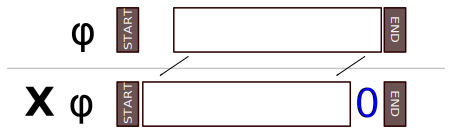
\includegraphics[scale=0.3]{Pattern-X}}~~~
\subfloat[$\mbox{\bf G}\,\varphi$]{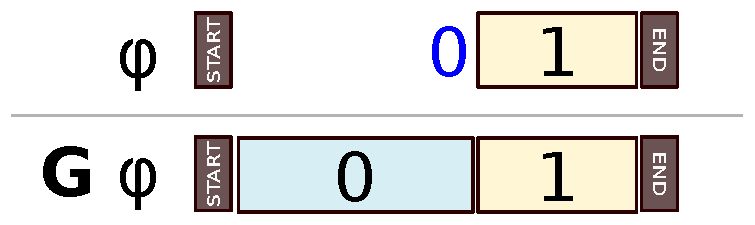
\includegraphics[scale=0.3]{Pattern-G}}~~~
\subfloat[$\varphi\,\mbox{\bf U}\,\psi$]{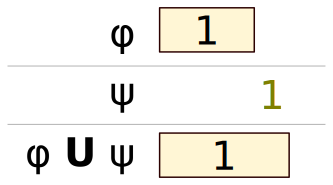
\includegraphics[scale=0.3]{Pattern-U}}
\caption{A graphical representation of the computation of three temporal operators on bitmaps}
\label{fig:patterns}
\end{figure}

\begin{algorithm}
\caption{Computing $\X a$}
\label{alg:next}
\begin{algorithmic}[1]
\Require Bitmap $a$
%\State // X(10101) $\Rightarrow$ (0101)
\State $out \gets$ removeFirstBit($a$)
\State addMany($out$, 0, 1)
\State \Return $out$
\end{algorithmic}
\end{algorithm}

To compute the vector for $\G\psi$, it suffices to find the smallest position $i$ such that all subsequent bits are 1. In $B_{\G\psi}$, all bits before $i$ are set to 0, and all bits after (and including) $i$ are set to 1. Thus to implement this operator using bitmaps, we need to do a search in the bitmap $B_{\psi}$ from back to front to find the last occurrence of the bit 0, as can be seen from Algorithm \ref{alg:global}. % and \ref{alg:future}.

Operator \textbf{F} (See Algorithm \ref{alg:future}) is the dual of \textbf{G}; its corresponding algorithm works in the same way as for \textbf{G}, swapping 0 and 1.

\begin{algorithm}
\caption{Computing $\G a$}
\label{alg:global}
\begin{algorithmic}[1]
\Require Bitmap $a$
\State $p \gets$ last(0, $a$)
\If {$p = -1$}
  \State \Return $a$
\Else
  \State $out \gets \langle~\rangle$
  \State addMany($out$, 0, $p + 1$)
  \State addMany($out$, 1, $|a| - p - 1$)
  \State \Return $out$
\EndIf
\end{algorithmic}
\end{algorithm}

\begin{algorithm}
\caption{\textbf{F}uture}
\label{alg:future}
\begin{algorithmic}[1]
\Require Bitmap $a$
%\State // F(010100) $\Rightarrow$ (111100)
\State $pos \gets$ last(1, $a$)
\If {$pos = -1$}
  \State \Return $a$
\Else
  \State $out \gets$ empty Bitmap
  \State addMany($out$, 1, $pos + 1$)
  \State addMany($out$, 0, $|a| - pos - 1$)
  \State \Return $out$
\EndIf
\end{algorithmic}
\end{algorithm}

According to Definition \eqref{eq:until}, if there is an index $j$ such that $\overline{s}^j \models \psi$ and $\overline{s}^i$ for all $i < j$, then $\overline{s}\models \varphi\U\psi$. In terms of bitmap operations, we need to keep checking if there is any bit set as 1 in $B_{\varphi}$ before every occurrence of bit 1 in $B_{\psi}$ (see Algorithm \ref{alg:until}).

\begin{algorithm}
\caption{Computing $a \U b$}
\label{alg:until}
\begin{multicols}{2}
\begin{algorithmic}[1]
\Require Bitmaps $a$ and $b$
\State $out \gets \langle~\rangle$
\State $p, a_0, a_1, b_0, b_1 \gets 0$
\While {$p < |a|$}
  \If {$a_1 \leq p$}
    \State $a_1 \gets$ next(1, $a$, $p$)
  \EndIf

  \If {$b_1 \leq p$}
    \State $b_1 \gets$ next(1, $b$, $p$)
  \EndIf

  \If {$a_1 = -1$ or $b_1 = -1$}
    \State \textbf{break}
  \EndIf

  \State $nearest1 \gets$ min($a_1$, $b_1$)
  \If {$nearest1 > p$}
    %\State // (00..) U (00..) $\Rightarrow$ (00..)
    \State addMany($out$, 0, $nearest1 - p$)
    \State $p \gets nearest1$
    \State \textbf{continue}
  \EndIf

  \If {$p = b_1$}
    %\State // (??..) U (11..) $\Rightarrow$ (11..)
    \If {$b_0 \leq b_1$}
      \State $b_0 \gets$ next(0, $b$, $b_1$)
      \If {$b_0 = -1$}
        \State $b_0 \gets |a|$
      \EndIf
    \EndIf
    \State addMany($out$, 1, $b_0 - p$)
    \State $p \gets b_0$
    \State \textbf{continue}
  \EndIf

  \If {$a_0 \leq a_1$}
    \State $a_0 \gets$ next(0, $a$, $a_1$)
    \If {$a_0 = -1$}
      \State $a_0 \gets |a|$
    \EndIf
  \EndIf
  \If {$a_0 \geq b_1$}
    %\State // (111?..) U (0001..) $\Rightarrow$ (1111..)
    \State addMany($out$, 1, $b_1 - p + 1$)
    \State $p \gets b_1 + 1$
  \Else
    %\State // (11100..) U (00001..) $\Rightarrow$ (00000..)
    \State addMany($out$, 0, $a_0 - p + 1$)
    \State $p \gets a_0 + 1$
  \EndIf
\EndWhile

\If {$b_1 = -1$}
  %\State // (..??) U (..00) $\Rightarrow$ (..00)
  \State addMany($out$, 0, $|a| - |out|$))
\ElsIf {$a_1 = -1$}
  %\State // (..0000) U (..1010) $\Rightarrow$ (..1010)
  \State copyTo($out$, $b$, $p$, $|a| - p$)
\EndIf

\State \Return $out$
\end{algorithmic}
  \end{multicols}
\end{algorithm}

The operation $\psi \textbf{ W } \varphi$ (Definition \eqref{eq:wuntil}) is quite like $\psi \textbf{ U } \varphi$, except that as the equation \eqref{eq:uw} \citep{huth2004} entails, the operation of the former also includes the operation $\textbf{G}\psi$. Algorithm \ref{alg:wuntil} explains its operation.

\begin{equation} \label{eq:uw}
\psi \textbf{W} \varphi \equiv \psi \textbf{U} \varphi \vee \textbf{G}\psi
\end{equation}

\begin{algorithm}
\caption{Computing $a \W b$}
\label{alg:wuntil}
\begin{multicols}{2}
\begin{algorithmic}[1]
\Require Bitmaps $a$ and $b$
\State $out \gets \langle~\rangle$
\State $p, a_0, a_1, b_0, b_1 \gets 0$
\While {p < |a|}
  \If {$a_1 \leq p$}
    \State $a_1 \gets$ next(1, $a$, $p$)
  \EndIf
  \If {$b_1 \leq p$}
    \State $b_1 \gets$ next(1, $b$, $p$)
  \EndIf
  \If {$a_1 = -1$ or $b_1 = -1$}
    \State \textbf{break}
  \EndIf

  \State $nearest1 \gets$ min($a_1$, $b_1$)
  \If {$nearest1 > p$}
    \State addMany($out$, 0, $nearest1 - p$)
    \State $p \gets nearest1$
    \State \textbf{continue}
  \EndIf

  \If {$p = b_1$}
    \If {$b_0 \leq b_1$}
      \State $b_0 \gets$ next(0, $b$, $b_1$)
      \If {$b_0 = -1$}
        \State $b_0 \gets |a|$
      \EndIf
    \EndIf
    \State addMany($out$, 1, $b_0 - p$)
    \State $p \gets b_0$
    \State \textbf{continue}
  \EndIf

  \If {$a_0 \leq a_1$}
    \State  $a_0 \gets$ next(0, $a$, $a_1$)
    \If {$a_0 = -1$}
      \State $a_0 \gets |a|$
    \EndIf
  \EndIf

  \If {$a_0 \geq b_1$}
    \State addMany($out$, 1, $b_1 - p + 1$)
    \State $p \gets b_1 + 1$
  \Else
    \State addMany($out$, 0, $a_0 - p + 1$)
    \State $p \gets a_0 + 1$
  \EndIf
\EndWhile

\If {$b_1 = -1$}
  \If {$a_1 = -1$}
    \State addMany($out$, 0, $|a| - |out|$)
  \Else
    \State $last0 \gets$ last(0, $a$)
    \If {$last0 = -1$ or $last0 < p$}
      \State addMany($out$, 1, $|a| - |out|$)
    \Else
      \State addMany($out$, 0, $last0 - p + 1$)
      \State addMany($out$, 1, $|a| - |out|$)
    \EndIf
  \EndIf
\ElsIf {$a_1 = -1$}
  \State copyTo($out$, $b$, $|b| - b_1 - 1$, $|b| - b_1$)
\EndIf

\State \Return $out$
\end{algorithmic}
\end{multicols}
\end{algorithm}

As the dual of the operator \textbf{U}, the operator \textbf{R} defined in \eqref{eq:release} need to union two parts for the formula $\psi \textbf{R} \varphi$: the first part aims to find whether exist $i, j (0 \leq i < j)$ which make $\pi^i, \pi^{i + 1}, ... \pi^j$ satisfy $\varphi$ when $\pi^j$ satisfies $\psi$; and the second is simply $G\varphi$. Algorithm \ref{alg:release} describes this procedure.

\begin{algorithm}
\caption{Computing $a \R b$}
\label{alg:release}
\begin{multicols}{2}
\begin{algorithmic}[1]
\Require Bitmaps $a$ and $b$
\State $out \gets \langle~\rangle$
\State $p, a_0, a_1, b_0, b_1 \gets 0$
\While {$p < |a|$}
  \If {$b_1 \leq p$}
    \State $b_1 \gets$ next(1, $b$, $p$)
  \EndIf
  \If {$b_1 = -1$}
    \State \textbf{break}
  \EndIf

  \If {$b_1 > p$}
    \State addMany($out$, 0, $b_1 - p$)
    \State $p \gets b_1$
    \State \textbf{continue}
  \EndIf

  \If {$a_1 \leq p$}
    \State $a_1 \gets$ next(1, $a$, $p$)
  \EndIf
  \If {$a_1 = -1$}
    \State \textbf{break}
  \EndIf

  \If {$b_0 \leq b_1$}
    \State $b_0 \gets$ next(0, $b$, $b_1$)
    \If {$b_0 = -1$}
      \State $b_0 \gets |a|$
    \EndIf
  \EndIf
  \If {$a_1 \geq b_0$}
    \State addMany($out$, 0, $b_0 - p + 1$)
    \State $p \gets b_0 + 1$
    \State \textbf{continue}
  \EndIf

  \If {$a_0 \leq a_1$}
    \State $a_0 \gets$ next(0, $b$, $a_1$)
    \If {$a_0 = -1$}
      \State $a_0 \gets |a|$
    \EndIf
  \EndIf
  \State $nearest0 \gets$ min($a_0$, $b_0$)
  \State addMany($out$, 1, $nearest0 - p$)
  \State $p \gets nearest0$
\EndWhile

\If {$a_1 = -1$ and $b_1 \neq -1$}
  \State $last0 \gets$ last(0, $b$)
  \If {$last0 = -1$ and $last0 < p$}
    \State addMany($out$, 1, $|a| - |out|$)
  \Else
    \State addMany($out$, 0, $last0 - p + 1$)
    \State addMany($out$, 1, $|a| - |out$)
  \EndIf
\Else
  \State addMany($out$, 0, $|a| - |out|$)
\EndIf

\State \Return $out$
\end{algorithmic}
\end{multicols}
\end{algorithm}

\subsection{Discussion}

An interesting point of this last algorithm is that the bitmaps $a$ and $b$ are not traversed in a linear fashion. Rather, entire blocks of each bitmap can be skipped to reach directly the next 0 or the next 1, depending on the case. Note that this is only possible if the trace is completely known in advance before starting to evaluate a formula (and moreover, the trace is traversed backwards). Therefore, our proposed solution is an example of an offline monitor that is not simply an online monitor that is fed events of a pre-recorded trace one by one: it exploits the possibility of \emph{random access} to parts of the trace that is only possible in an offline setting.

This example shows one of the advantages of our proposed technique in terms of complexity. Indeed, reading the original log to create the ground bitmaps can be done in linear time (and in a single pass for all propositional symbols at once). However, once these initial bitmaps are computed, many of the required operations do not require a linear processing of the trace anymore. For example, evaluating $\X\varphi$ requires a simple bit shift, which can be done in a single CPU operation for 64 bits at a time, and potentially much more if compression is used.\footnote{The left bit shift of a compressed block is the block itself, as long as the next bit to the right has the same value.} Similarly, looking for the next 0 or 1 seldom requires linear searching, as the use of compression makes it possible to skip over fill words in one operation. Computing the bitmap for a \textbf{F} or \textbf{G} operator requires a single such lookup for the entire trace.

Another interesting point is the fact that operators \textbf{F} and \textbf{G} are monotonous. As can be seen in Figure \ref{fig:patterns}, the resulting bitmap is of the form $0^*1^*$ (or the reverse). Hence a very simple bitmap is propagated upwards to further algorithms; it can be heavily compressed, and makes any lookup for the next 0 or the next 1 trivial. While not producing such simple vectors, bitmaps resulting from the application of \textbf{U} still have a relatively regular structure that is again amenable to reasonable compression.

%% }}} --- Subsection

%% }}} --- Section

%% ------------------
%% Section: expériences
%% ------------------
\section{Implementation and Experiments}\label{sec:bm:experiments} %% {{{

While the worst-case complexity of every algorithm presented in the previous section is still $O(n)$ (where $n$ is the size of the input bitmap), we suspect that performance in practice should be much better. Therefore, in this section, we describe experiments in order to achieve the following purposes:

\begin{enumerate}
\item Test the performance of fundamental LTL algorithms
\item Test the performance of the recursive application of these algorithms on complex LTL formul\ae{}
\item Evaluate the performance and space savings incurred by the use of compression
\end{enumerate}

\begin{comment}
\subsection{Modifications to Libraries} %% {{{

Section \ref{sec:bm:ltlbitmap} mentions that the time and space complexities of all LTL operators are $O(n)$ where $n$ is the size of the input uncompressed bitmap. After applying RLE-model bitmap compression algorithms to our solution, the space complexities become $O(m)$ as is discussed above, and we managed to make the time complexities also become $O(m)$ by implementing the bitmap manipulation functions listed in Table \ref{tbl:bm:bmhelpers} for every  bitmap compression algorithms.

Because of lack of the support of random access for the RLE-model bitmap compression algorithms, we cannot enumerate the bits in the same way as uncompressed bitmap. Therefore we design an \emph{iterator} data structure to store not only the absolute index of current bit in the uncompressed bitmap but also the relative index in the compressed bitmap.

Taking the function \textbf{next(1, )} as an example, if the current relative index is in a sequence word of 0, the search in this word is unnecessary, and we just jump to the next word; if the index is in a sequence word of 1, we return the current index; however, if the index is in a literal word, we have to look for the bit 1 in the $ulen$-bits word.

%% }}}
\end{comment}

\subsection{Experimental Setup} %% {{{

As a means to avoid the runtime disk I/O cost we load all relevant files into memory before the calculations. Thus although using bitmap can considerably reduce the requirement of memory, we prepared a workstation with an Intel Xeon E5-2630 v3 Processor and 48 GB of memory.

All codes are implemented in Java which self takes responsibility of the memory management and garbage collection. Concerning the delay caused by garbage collection (GC) and especially Full-GC, we called \textit{System.gc()} before and after every formula calculation to provide a runtime environment that was as ``clean'' as possible.

Table \ref{table:bmlibs} shows the libraries used for different types of bitmap. In order to implement all the LTL operations, we modified the codes of the libraries to add the necessary functions listed in Table \ref{tbl:bm:bmhelpers} and to optimize the functions so that the time complexities of the operators become $O(m)$ where $m$ is the number of sequences of consecutive 0/1 bits.

\begin{table}
\centering
\begin{tabular}{|c|l|}
\hline
Bitmap & Source \\
\hline
Uncompressed & \texttt{java.util.BitSet} from Java SDK \\
\hline
\multirow{2}{*}{WAH} & Original:\ \ \url{https://github.com/metamx/extendedset} \\
& Modified: \url{https://github.com/phoenixxie/extendedset} \\
\hline
\multirow{2}{*}{Concise} & Original:\ \ \url{https://github.com/metamx/extendedset} \\
& Modified: \url{https://github.com/phoenixxie/extendedset} \\
\hline
\multirow{2}{*}{EWAH} & Original:\ \ \url{https://github.com/lemire/javaewah} \\
& Modified: \url{https://github.com/phoenixxie/javaewah} \\
\hline
Roaring & \url{https://github.com/lemire/RoaringBitmap} \\
\hline
\end{tabular}
\caption{Bitmap libraries}
\label{table:bmlibs}
\end{table}

Because of lack of the support of random access for the RLE-model bitmap compression algorithms, we cannot enumerate the bits in the same way as for an uncompressed bitmap. Therefore we designed an \emph{iterator} data structure to store not only the absolute index of current bit in the uncompressed bitmap but also the relative index in the compressed bitmap. Taking the function \textbf{next(1,x)} as an example, if the current relative index is in a sequence word of 0, the search in this word is unnecessary, and we just jump to the next word; if the index is in a sequence word of 1, we return the current index; however, if the index is in a literal word, we have to look for the bit 1 in the $ulen$-bits word.

For the experiments, we developed a random data generator. Every time it generates $5 \times 10^7$ tuples, and each tuple contains 3 random numbers ($a, b, c$) related with 3 simple inequalities: $a > 0$, $b > 0$ and $c \leq 0$, which will be labelled as $s_0$, $s_1$ and $s_2$, respectively. According to \eqref{eq:ap}, the true/false values of these 3 statements consist of the atomic propositions. When a tuple was passed to the 3 statements, we got 3 boolean values each of which was then turned into a 1/0 bit in the bitmap corresponding to one of the 3 statements. When all tuples were processed, we had 3 bitmaps having 50 million bits each.

% The experiment data was a file with 50 million lines of states, each of which contained 3 random numbers used for 3 relational statements. The true/false values of these 3 statements $(s_0, s_1, s_2)$ consisted of the atomic propositions.

% \begin{table}
% \centering
% \begin{tabular}{|c|c|}
% \hline
% & Relational statement \\
% \hline
% $s_0$ & $a > 0$ \\
% \hline
% $s_1$ & $b > 0$ \\
% \hline
% $s_2$ & $c \leq 0$ \\
% \hline
% \end{tabular}
% \caption{Relational statements}
% \label{tbl:bm:statements}
% \end{table}

% Pas vraiment pertinent --SH
% The range of the random numbers is [-10000, 10000], and according to the three inequalities mentioned earlier, it is easy to know that the difference between the probabilities of getting 1 and getting 0 is only about $0.05\permil$ if the random function is fair enough, therefore there should be nearly the same number of 1 and 0 bits in the generated bitmap.

\subsection{Basic LTL Operators} %% {{{

A first experiment consisted of evaluating the performance, in terms of computation time, for evaluating a bit vector on each propositional and temporal operator taken separately.

In the first experiment, we ran 100 passes of a benchmark on the fundamental operators with uncompressed bitmaps. In every pass, the experiment data was regenerated and passed to the relational statements from which the bitmaps were created. Then the formul\ae{} were executed with the bitmaps. In the final step we calculated the average running time of a pass for each LTL operator, and the number of bits processed per second.

Table \ref{tbl:bm:basicops} shows that the propositional logic operators were faster than most temporal logic operators. Among the temporal logic operators, the binary operators were slower than the unary ones because the former require more operations than the latter, especially in the situation that many 0s and 1s sequences are mixed in the bitmap. The dual operators \textbf{G} and \textbf{F} have similar algorithms but \textbf{F} surprisingly took three times longer than \textbf{G}. This can be explained by the fact that for a fairly-randomized input bitmap, \textbf{F} will append more 1s than 0s to its output bitmap, while \textbf{G} will append more 0s than 1s. Although the Java \texttt{BitSet} implementation supports both to set a bit to 1 and to clear a bit to 0\footnote{\url{https://docs.oracle.com/javase/8/docs/api/java/util/BitSet.html}}, it actually does nothing when clearing a new bit of which the index is beyond its size, i.e. appending a bit 0. This results in an asymmetrical processing of 0s and 1s in the bitmap.

\begin{table}
\centering
\small
\begin{tabular}{|c|c|c|c|c|}
\hline
Formula & Min.\ time & Max.\ time & Avg.\ time & Throughput \\
& (ms) & (ms) & (ms) & (b/s) \\
\hline
$\neg s_0$ & 0 & 15 & 6.18 & $8.09 \times 10^{9}$ \\
\hline
$s_0 \wedge s_1$ & 0 & 16 & 5.86 & $8.53 \times 10^{9}$ \\
\hline
$s_0 \vee s_1$ & 0 & 16 & 5.8 & $8.62 \times 10^{9}$ \\
\hline
$s_0 \rightarrow s_1$ & 0 & 16 & 4.66 & $1.07 \times 10^{10}$ \\
\hline
$\X s_0$ & 0 & 16 & 8.93 & $5.60 \times 10^{9}$ \\
\hline
$\G s_0$ & 46 & 63 & 51.3 & $9.75 \times 10^8$ \\
\hline
$\F s_0$ & 140 & 174 & 150.55 & $3.32 \times 10^8$ \\
\hline
$s_0 \U s_1$ & 1562 & 2017 & 1747.05 & $5.72 \times 10^7$ \\
\hline
$s_0 \W s_1$ & 1531 & 1957 & 1685.71 & $5.93 \times 10^7$ \\
\hline
$s_0 \R s_1$ & 1735 & 2188 & 1961.37 & $5.10 \times 10^7$ \\
\hline
\end{tabular}
\vskip 8pt
\caption{Running time for evaluating each LTL operator on a bit vector, without the use of a compression library.}
\label{tbl:bm:basicops}
\end{table}

%% }}} --- Subsection

\subsection{Complex formul\ae{}} %% {{{

The results from this first experiment suggest that propositional logic operators, temporal logic unary operators and temporal logic binary operators have different magnitudes of processing speed; therefore we can divide the operators into three groups.

At the beginning of this second experiment, we composed various combinations of operators into 14 LTL formul\ae{} with the help of the tool \emph{randltl} from the library \textit{Spot} \footnote{\url{https://spot.lrde.epita.fr/index.html}}; the formul\ae{} are shown in Table \ref{tbl:bm:complex-formulas}. Then we also ran a 50-pass benchmark on the these formul\ae{} with uncompressed bitmaps. In each cycle the data was regenerated and re-executed with the 14 formul\ae{}. We measured the running time of each cycles and calculated the average time cost and the processing speed as before.


\begin{table}[h]
%\begin{footnotesize}

\begin{equation}\tag{F1}
\G ((s_2 \mathrel{\rightarrow} \F (\mathop{\neg}(s_1 \U  s_2) \W  (s_2 \mathrel{\vee} \G s_1))) \W  (\mathop{\neg}\F (s_0 \R  \X s_2) \W  ((s_0 \mathrel{\wedge} s_2 \mathrel{\wedge} \F s_2) \U  s_0)))
\end{equation}
%
\squeeze
%
\begin{equation}\tag{F2}
\F (\mathop{\neg}(s_2 \mathrel{\rightarrow} \X (s_0 \U  s_1)) \U  (\mathop{\neg}(s_0 \mathrel{\vee} \F \X (s_0 \U  (\X (\F s_1 \W  s_1) \R  s_1))) 
\U  (s_0 \R  \G s_2)))
\end{equation}
%
\squeeze
%
\begin{equation}\tag{F3}
\X \F ((s_1 \mathrel{\vee} s_2 \mathrel{\vee} (\G (s_0 \mathrel{\vee} s_1 \mathrel{\vee} \mathop{\neg}s_1) \mathrel{\wedge} \X \mathop{\neg}s_0)) \mathrel{\rightarrow} \\
((\mathop{\neg}s_0 \mathrel{\rightarrow} (s_0 \mathrel{\wedge} \mathop{\neg}s_1)) \mathrel{\wedge} \G s_0))
\end{equation}
%
\squeeze
%
\begin{equation}\tag{F4}
\X (\mathop{\neg}\G (s_0 \mathrel{\rightarrow} s_2) \mathrel{\rightarrow} \F (s_1 \mathrel{\wedge} ((\F (s_0 \mathrel{\wedge} s_2) \mathrel{\rightarrow} s_1) \mathrel{\rightarrow} \X \mathop{\neg}s_2) \mathrel{\wedge} \G (s_2 \mathrel{\rightarrow} (s_2 \mathrel{\wedge} \F s_1))))
\end{equation}
%
\squeezemore
%
\begin{multline}\tag{F5}
\mathop{\neg}((s_0 \U  (\mathop{\neg}(\mathop{\neg}s_0 \mathrel{\wedge} s_2) \mathrel{\vee} (\mathop{\neg}s_0 \W  (s_2 \mathrel{\rightarrow} s_0)))) \\
\W  \mathop{\neg}s_0) \mathrel{\vee}
(s_1 \R  ((s_1 \mathrel{\vee} (s_0 \W  s_2)) \W  (\mathop{\neg}s_0 \W  s_2)))
\end{multline}
%
\squeeze
%
\begin{equation}\tag{F6}
(s_1 \W  ((s_2 \mathrel{\rightarrow} (\mathop{\neg}s_2 \R  \mathop{\neg}(\mathop{\neg}s_1 \W  s_0))) \W  (\mathop{\neg}s_1 \mathrel{\vee} \mathop{\neg}((\mathop{\neg}s_2 \mathrel{\rightarrow} s_1) \mathrel{\rightarrow} \mathop{\neg}s_0)))) \W  (s_0 \R  \mathop{\neg}s_2)
\end{equation}
%
\squeezemore
%
\begin{multline}\tag{F7}
\X (((\F s_2 \R  s_0) \U  \F s_0) \R  \G ((s_2 \W  s_1) \W  \\
(((\G s_2 \U  s_1) \R  \X s_0) \R  (s_2 \W  ((s_2 \R  \X s_2) \W  s_1)))))
\end{multline}
%
\squeezemore
%
\begin{equation}\tag{F8}
(\G (s_0 \R  \F s_1) \U  \F s_2) \W  \G ((s_1 \U  s_2) \R  ((\G \X s_0 \U  (s_2 \W  s_0)) \W  \F ((\G s_1 \U  s_2) \R  s_2)))
\end{equation}
%
\squeeze
%
\begin{equation}\tag{F9}
\G \F (\G \F s_0 \mathrel{\wedge} \F \X \G s_1 \mathrel{\wedge} \G \F \X \X \X \G \X \F \G s_2)
\end{equation}
%
\squeeze
%
\begin{equation}\tag{F10}
\F \G \F \X (\X s_2 \mathrel{\wedge} \X \G \X \X \G \F (\G \X \F s_1 \mathrel{\wedge} \X \G s_0))
\end{equation}
%
\squeeze
%
\begin{equation}\tag{F11}
\mathop{\neg}(((s_0 \mathrel{\vee} s_2) \mathrel{\rightarrow} (\mathop{\neg}(s_2 \mathrel{\wedge} (\mathop{\neg}s_2 \mathrel{\rightarrow} \mathop{\neg}(s_0 \mathrel{\wedge} (s_0 \mathrel{\vee} \mathop{\neg}s_1)))) \mathrel{\vee} (s_0 \mathrel{\wedge} \mathop{\neg}s_0))) \mathrel{\vee} (\mathop{\neg}s_0 \mathrel{\wedge} (s_0 \mathrel{\vee} s_2)))
\end{equation}
%
\squeezemore
%
\begin{multline}\tag{F12}
(s_1 \mathrel{\wedge} \mathop{\neg}s_2 \mathrel{\wedge} (s_2 \mathrel{\rightarrow} s_0)) \mathrel{\vee} \mathop{\neg}((s_0 \mathrel{\wedge} \mathop{\neg}s_0) \mathrel{\rightarrow} s_1) \mathrel{\vee} \\
((s_2 \mathrel{\vee} (s_1 \mathrel{\rightarrow} s_0)) \mathrel{\wedge} ((s_0 \mathrel{\wedge} \mathop{\neg}s_2 \mathrel{\wedge} (s_1 \mathrel{\rightarrow} s_0)) \mathrel{\rightarrow} s_0))
\end{multline}
%
\squeezemore
%
\begin{multline}\tag{F13}
(((s_0 \W  s_2) \W  s_0) \U  ((s_1 \U  (((s_1 \W  s_2) \W  (s_1 \R  (s_1 \R  s_0))) \W  s_2)) \W  s_2)) \W  \\
((s_0 \R  s_1) \R  (((s_2 \U  s_1) \U  s_1) \R  ((s_0 \W  s_2) \W  s_1)))
\end{multline}
%
\squeezemore
%
\begin{multline}\tag{F14}
((((s_1 \U  s_2) \U  (s_2 \U  s_1)) \U  s_1) \R  (s_1 \R  s_2)) \U  (((s_2 \W  ((s_0 \W  \\
((s_2 \R  s_0) \R  s_1)) \U  s_1)) \W  s_0) \W  (((s_0 \R  s_1) \R  (s_0 \W  s_1)) \U  s_0))
\end{multline}

%\end{footnotesize}
\vskip 8pt
\caption{The complex LTL formul\ae{} evaluated experimentally.}
\label{tbl:bm:complex-formulas}
\end{table}

As is indicated in Table \ref{tbl:bm:complex}, 3 groups of operators have different scales of processing speed. The combinations having temporal logic and binary operators always took more time than others, and formul\ae{} 13 and 14 are the slowest. This result also shows that our solution can handle a fairly large number of bits (events from the trace) per second, ranging from millions to billions.

\begin{table}[h]
\centering
\small
\begin{tabular}{|c|c|c|c|c|c|c|c|}
\hline
Formula & Prop. & Temp. & Temp. & Min Time & Max Time & Avg. Time & Approx. \\
No. & Logic & Unary & Binary & (ms) & (ms) & (ms) & bits/second \\
& Ops. & Ops. & Ops. & & & & \\
\hline
F1 & 6 & 6 & 6 & 10454 & 14205 & 11483.02 & $1.31 \times 10^7$ \\
\hline
F2 & 4 & 7 & 7 & 7728 & 10673 & 8937.59 & $1.68 \times 10^7$  \\
\hline
F3 & 13 & 5 & 0 & 281 & 422 & 326.63 & $4.59 \times 10^8$  \\
\hline
F4 & 11 & 7 & 0 & 422 & 704 & 560.58 & $2.68 \times 10^8$  \\
\hline
F5 & 11 & 0 & 7 & 8532 & 10496 & 9374.5 & $1.60 \times 10^7$  \\
\hline
F6 & 12 & 0 & 6 & 7280 & 9357 & 7934.6 & $1.89 \times 10^7$  \\
\hline
F7 & 0 & 7 & 11 & 12330 & 15004 & 13413.91 & $1.18 \times 10^7$  \\
\hline
F8 & 0 & 8 & 10 & 9442 & 11833 & 10428.37 & $1.44 \times 10^7$  \\
\hline
F9 & 2 & 16 & 0 & 431 & 1155 & 682.68 & $2.20 \times 10^8$  \\
\hline
F10 & 2 & 16 & 0 & 375 & 857 & 472.76 & $3.17 \times 10^8$  \\
\hline
F11 & 18 & 0 & 0 & 31 & 56 & 45.18 & $3.32 \times 10^9$  \\
\hline
F12 & 18 & 0 & 0 & 46 & 68 & 51.58 & $2.91 \times 10^9$  \\
\hline
F13 & 0 & 0 & 18 & 22768 & 27308 & 24825.21 & $6.04 \times 10^6$  \\
\hline
F14 & 0 & 0 & 18 & 22800 & 27481 & 24877.67 & $6.03 \times 10^6$  \\
\hline
\end{tabular}
\vskip 8pt
\caption{Running time for the evaluation of LTL formul\ae{} of Table \ref{tbl:bm:complex-formulas}, without the use of a compression library.}
\label{tbl:bm:complex}
\end{table}

%% }}} --- Subsection

\subsection{Use of Bitmap Compression} %% {{{

According to the RLE-model algorithms, the compression ratio mostly depends on the length of consecutive 0s or 1s. Hence in this experiment we modified the generator to enable it to repeat the same tuple a specified number of times: 1, 32 and 64. This new mechanism is able to ensure the existence of continuous sequences with a minimum length ($slen$) in the generated bitmaps. Intuitively, when the value of $slen$ increases, the number of sequences decreases; therefore the RLE-model algorithms can be expected to have better performance than an uncompressed bitmap. % for its $O(m)$ time and space complexities.

\begin{figure}[h]
\begin{center}
\centering
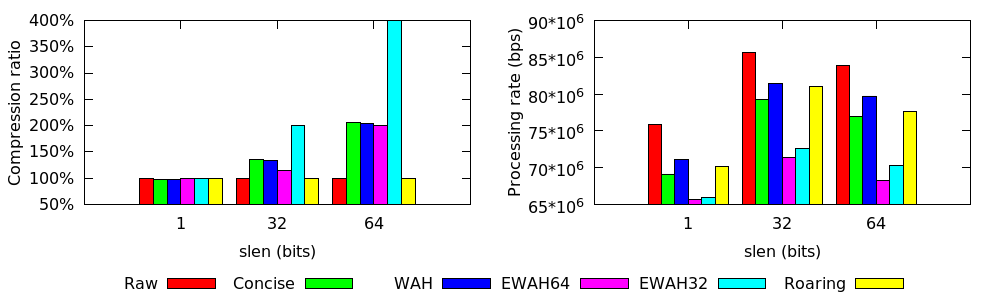
\includegraphics[width=\linewidth]{states.png}
\caption{Bitmap generation with compression algorithms}
\label{img:states}
\end{center}
\end{figure}

In the first part of the experiment, we generated the bitmaps with different algorithms and different values of $slen$, and then calculated the compression ratios. The result in Figure \ref{img:states} confirms the hypothesis that when $slen < wlen$ (where $wlen$ is the length of a word), the bitmap cannot be well compressed by any RLE-model algorithm, and in this case, the algorithm EWAH behaves a little better than the others due to its smaller structural cost. When $slen$ increases to 32 and 64, i.e. $slen \geq wlen$, the RLE algorithms start to work well and the compression ratio of $slen = 64$ is obviously better than the one of $slen = 32$. From the figure \ref{img:states} we can also see that when $slen$ is 1, 32 and 64, EWAHs are much slower than WAH, Concise and Roaring.

\begin{comment}
The result in Figure \ref{img:ratio} shows that when the length of consecutive bits is small ($\leq 5$), there is no great gap of the ratio among the RLE-model algorithms, Roaring bitmap and even uncompressed bitmap. The word lengths of WAH, Concise, EWAH(32bit), EWAH(64bit) are 32, 32, 32 and 64, so when the length grows beyond 50, which is over 32 and slightly less than 64, the ratios increase dramatically. The compression ratio of Roaring bitmap depends on the fraction of 1s bits in the bitmap, when the bitmap is not very sparse, the algorithm has to allocate much memory for its containers which in our opinion is the reason that its compression ratio is near 1 (uncompressed).
\end{comment}

In the second part of the experiment, we measured the performance of the compressed bitmaps when applying the algorithms for all fundamental operators and all LTL formul\ae{}s in the previous experiments. Detailed results covering all the operators and formul\ae{}s can be found in Appendix \ref{appendixa}.

To this end, we picked formula F1 and F14 from the previous experiment, as F1 contains all the operators and connectives of LTL and F14 is the slowest of all formul\ae{} in the previous experiment. We again ran the benchmark 100 passes; in each cycle, the formula was evaluated with one group of input bitmaps from the last step and we recorded the time cost of each bitmap algorithm and each length of consecutive bits.

\begin{figure}[h]
\begin{center}
\centering
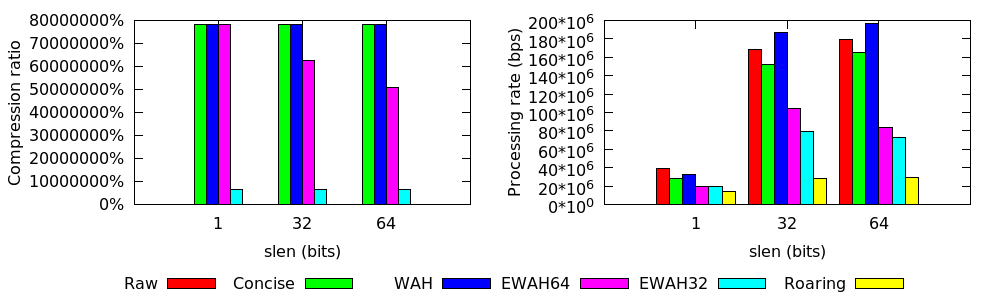
\includegraphics[width=\linewidth]{p11.png}
\caption{Comparison of compression ratio and processing rate for LTL formula 1, for various bitmap compression libraries and various values of $slen$}
\label{img:f1}
\end{center}
\end{figure}

\begin{figure}[h]
\begin{center}
\centering
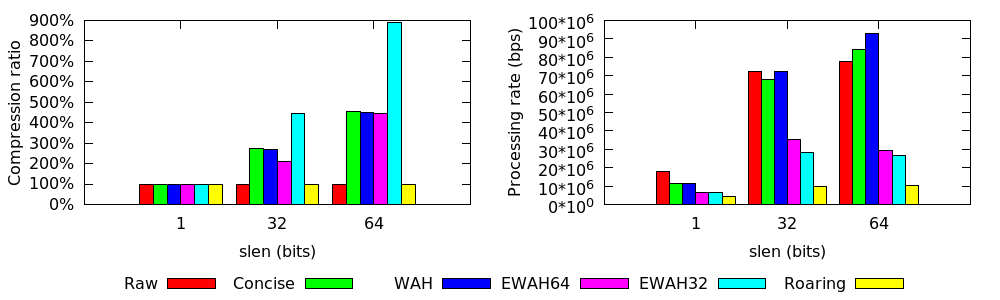
\includegraphics[width=\linewidth]{p24.png}
\caption{Comparison of compression ratio and processing rate for LTL formula 14, for various bitmap compression libraries and various values of $slen$}
\label{img:f14}
\end{center}
\end{figure}

According to Figure \ref{img:f1} and \ref{img:f14}, the performance of the RLE-model algorithms, WAH, EWAH and Concise is obviously related to the value of $slen$. The Figure \ref{img:f1} also suggests that the presence of operators \textbf{G} and \textbf{F} can vastly increase the length of consecutive bits of same value, which in turn can be well compressed by RLE-model algorithms. In such a case, several algorithms have better performance than the uncompressed bitmap as $slen$ increases.

%% }}} --- Subsection

%% }}} --- Section

%% ------------------
%% Section: related work
%% ------------------
\section{Related Work}\label{sec:bm:related} %% {{{

The prospect of using physical properties of hardware to boost the performance of runtime verification has already been studied in the recent past. For example, Pellizzoni \etal\@ \citep{pellizzoni2008hardware} utilized dedicated commercial-off-the-shelf (COTS) hardware \citep{emerson1990temporal} to facilitate the runtime monitoring of critical embedded systems whose properties were expressed in Past-time Temporal Linear Logic (PTLTL).

As the number of cores (GPU or multi-core CPUs) in the commodity hardware keeps increasing, the research of exploiting the available processors or cores to parallelize the tasks and the computing  brings a challenge and also an opportunity to improve the architecture of runtime verification. For example, Ha \etal\@ \citep{ha2009concurrent} introduced a buffering design of \emph{Cache-friendly Asymmetric Buffering (CAB)} to improve the communications between application and runtime monitor by exploiting the shared cache of the mutilcore architecture; Berkovich \etal\@ \citep{DBLP:journals/fmsd/BerkovichBF15} proposed a GPU-based solution that effectively utilizes the available cores of the GPU, so that the monitor designed and implemented with their method can run in parallel with the target program and evaluate LTL properties.

Previous work by one of the authors \citep{jocasa} introduced an algorithm for the automated verification of Linear Temporal Logic formul\ae{} on event traces, using an increasingly popular cloud computing framework called MapReduce. The algorithm can process multiple, arbitrary fragments of the trace in parallel, and compute its final result through a cycle of runs of MapReduce instances.
The proposed technique manipulates objects called \emph{tuples}, which are of the form $\langle \phi, (n, i)\rangle$, and are interpreted as the statement ``the process is at iteration $i$, and LTL formula $\phi$ is true for the suffix of the current trace starting at its $n$-th event''. One can see that this statement corresponds exactly to the fact, in the present solution, that the $n$-th position of the bitmap generated by the evaluation of $\phi$ contains the value 1.

Apart from this similarity, however, the two techniques are radically different. Since the MapReduce approach operates on tuples one by one, while the present solution manipulates entire bitmaps, the algorithms for each LTL operator have little in common (especially that for \textbf{U}). Where the MapReduce approach gets its speed from the processing of multiple subformul\ae{} on different machines, our present solution is efficient because some operations (such as conjunction) can be computed simultaneously for many adjacent events in a single CPU cycle. In addition, a downside of the MapReduce solution is the large number of tuples generated, and the impossibility of compressing that volume of data.

As one can see, there have been multiple attempts at leveraging parallelism and properties of hardware to evaluate temporal expressions on traces. However, As far as we know, our work it the first to get its performance boost at the level of the \emph{data structures} used to evaluate these expressions.

%% }}} --- Section

%% ------------------
%% Section: conclusion
%% ------------------
\section{Conclusion and future work}\label{sec:bm:conclusion} %% {{{

We proposed a solution for the offline evaluation of LTL formul\ae{} by means of bitmap manipulations. In such a setting, propositional predicates on individual events of a trace states are mapped to bits of a vector (``bitmap'') that are then manipulated to implement each LTL operator. In addition to the fact that bitmap manipulations are in themselves very efficient, our algorithms take advantage of the fact that the trace is completely known in advance, and that random access to any position of that trace makes it possible to skip large blocks of events to speed up the evaluation.

For this reason, our solution is a prime example of an offline evaluation algorithm that exploits the fact that it indeed works offline ---it is not merely an online algorithm that reads events from a pre-recorded trace one by one. As a matter of fact, in some cases (such as the \textbf{U} operator), the trace is even evaluated from the end, rather than from the beginning. A thorough performance benchmark for both fundamental operators and complex LTL formul\ae{} proved the feasibility of the approach, and showed how events from a trace can be processed at a rate ranging from millions to billions of events per second.

To further exploit the potential of bitmaps, we introduced bitmap compression algorithms in our solution and integrated them in our benchmark. In the experiments, as we expected, compressed bitmaps demonstrated thair ability to easily compress sparse bitmaps and accelerating the LTL operations when there is a certain amount of consecutive bits with the same value. We have explained, how many LTL operators naturally increase the regularity of the bitmaps they are processing.

Obviously, this solution is suitable only for offline evaluation. However, The promising results obtained in our implementation lead to a number of potential extensions and improvements over the current method. First, the algorithm can be reused as a basis for other temporal languages that intersect with LTL, such as PSL \cite{IntroPSLBook}. Second, the technique could be expanded to take into account data parameters and quantification. Finally, one could also consider to parallellize the evaluation of large segments of btimaps on multiple machines.

%% }}} --- Section

%% :folding=explicit:wrap=soft:mode=latex:


%% ...
%% Ajoutez autant de commandes include qu'il y a de chapitres à
%% inclure dans votre document
%% ...
%% La conclusion n'est pas numérotée
\chapter{Conclusion}

Lorem ipsum dolor sit amet, consectetur adipiscing elit. Aenean ac
ullamcorper mi. Vivamus non turpis odio. Cras vel mauris mauris. Vivamus
augue justo, fringilla vitae placerat a, rutrum placerat mi. Mauris in
ligula in velit aliquam sodales eu ac est. Phasellus elementum interdum
lectus id congue. Nullam eget rutrum augue.

Quisque ut tellus nulla. Phasellus ut turpis quis erat semper pharetra.
Donec consectetur vehicula dui id pretium. In et massa lectus. Nulla mattis
pulvinar convallis. Etiam at odio velit. Phasellus eleifend, neque vel
euismod rutrum, turpis orci gravida velit, vel placerat arcu lectus quis
nisl. Vivamus vel mauris justo. Donec facilisis facilisis sem, in vestibulum
quam imperdiet eget. Sed tortor justo, adipiscing a tincidunt at, pharetra
vitae felis. Ut quis orci leo, id suscipit leo. Maecenas tincidunt lectus et
risus tempus non tristique libero tempor. In arcu sapien, suscipit ac tempor
eu, venenatis ut tellus. Nullam metus felis, tempor id scelerisque tempor,
fermentum non nisl. Nulla viverra ultricies neque sit amet facilisis.
  


% \begin{appendices}
% %!TEX root = these.tex

In this appendix, we present the experiment results of the third part of Section \ref{sec:bm:experiments}. To get better formatting, the data format is different than it in Section \ref{sec:bm:experiments}. ``Ratio'' here has not percentage mark because it is compression rate calculated by the division of original data size and compressed size.

\begin{table}[h]
\small
\centering
\makebox[\linewidth]{
\begin{tabular}{|c|c|c|c|c|c|c|c|c|c|c|}
\hline
& $slen$ & \multicolumn{3}{|c|}{1} & \multicolumn{3}{|c|}{32} & \multicolumn{3}{|c|}{64} \\
\hline
Type & & Min & Max & Avg. & Min & Max & Avg. & Min & Max & Avg. \\
\hline
\multirow{2}{*}{Raw} & Ratio & 1.00 & 1.00 & 1.00 & 1.00 & 1.00 & 1.00 & 1.00 & 1.00 & 1.00 \\
\cline{2-11}
& bps & 6.44E+7 & 8.32E+7 & 7.59E+7 & 7.64E+7 & 9.18E+7 & 8.57E+7 & 7.40E+7 & 9.27E+7 & 8.39E+7 \\
\hline
\multirow{2}{*}{Concise} & Ratio & 0.97 & 0.97 & 0.97 & 1.35 & 1.35 & 1.35 & 2.06 & 2.07 & 2.07 \\
\cline{2-11}
& bps & 6.18E+7 & 7.60E+7 & 6.91E+7 & 6.99E+7 & 8.56E+7 & 7.93E+7 & 6.67E+7 & 8.47E+7 & 7.70E+7 \\
\hline
\multirow{2}{*}{WAH} & Ratio & 0.97 & 0.97 & 0.97 & 1.33 & 1.34 & 1.33 & 2.03 & 2.04 & 2.03 \\
\cline{2-11}
& bps & 6.28E+7 & 7.84E+7 & 7.12E+7 & 7.23E+7 & 8.86E+7 & 8.15E+7 & 6.58E+7 & 8.95E+7 & 7.97E+7 \\
\hline
\multirow{2}{*}{EWAH64} & Ratio & 1.00 & 1.00 & 1.00 & 1.14 & 1.14 & 1.14 & 1.99 & 2.01 & 2.00 \\
\cline{2-11}
& bps & 5.66E+7 & 7.29E+7 & 6.56E+7 & 6.24E+7 & 7.62E+7 & 7.14E+7 & 5.99E+7 & 7.58E+7 & 6.83E+7 \\
\hline
\multirow{2}{*}{EWAH32} & Ratio & 1.00 & 1.00 & 1.00 & 2.00 & 2.00 & 2.00 & 3.99 & 4.01 & 4.00 \\
\cline{2-11}
& bps & 5.82E+7 & 7.34E+7 & 6.59E+7 & 6.48E+7 & 7.74E+7 & 7.26E+7 & 6.09E+7 & 7.73E+7 & 7.03E+7 \\
\hline
\multirow{2}{*}{Roaring} & Ratio & 1.00 & 1.00 & 1.00 & 1.00 & 1.00 & 1.00 & 1.00 & 1.00 & 1.00 \\
\cline{2-11}
& bps & 6.11E+7 & 7.78E+7 & 7.01E+7 & 7.04E+7 & 8.72E+7 & 8.10E+7 & 6.78E+7 & 8.88E+7 & 7.76E+7 \\
\hline
\end{tabular}
}
\caption{Bitmap generation with compression algorithms}
\end{table}

\begin{table}[h]
\small
\centering
\makebox[\linewidth]{
\begin{tabular}{|c|c|c|c|c|c|c|c|c|c|c|}
\hline
& $slen$ & \multicolumn{3}{|c|}{1} & \multicolumn{3}{|c|}{32} & \multicolumn{3}{|c|}{64} \\
\hline
Type & & Min & Max & Avg. & Min & Max & Avg. & Min & Max & Avg. \\
\hline
\multirow{2}{*}{Raw} & Ratio & 1.00 & 1.00 & 1.00 & 1.00 & 1.00 & 1.00 & 1.00 & 1.00 & 1.00 \\
\cline{2-11}
& bps & 3.00E+10 & 4.50E+11 & 7.28E+10 & 4.50E+10 & 7.50E+10 & 5.79E+10 & 2.65E+10 & 6.43E+10 & 5.17E+10 \\
\hline
\multirow{2}{*}{Concise} & Ratio & 0.97 & 0.97 & 0.97 & 1.35 & 1.35 & 1.35 & 2.06 & 2.07 & 2.07 \\
\cline{2-11}
& bps & 7.37E+9 & 3.32E+10 & 1.24E+10 & 1.45E+10 & 2.09E+10 & 1.84E+10 & 1.04E+10 & 1.68E+10 & 1.35E+10 \\
\hline
\multirow{2}{*}{WAH} & Ratio & 0.97 & 0.97 & 0.97 & 1.33 & 1.34 & 1.33 & 2.03 & 2.04 & 2.03 \\
\cline{2-11}
& bps & 9.48E+9 & 4.65E+11 & 1.80E+10 & 3.75E+10 & 4.82E+10 & 4.34E+10 & 3.16E+10 & 4.43E+10 & 3.84E+10 \\
\hline
\multirow{2}{*}{EWAH64} & Ratio & 1.00 & 1.00 & 1.00 & 1.14 & 1.14 & 1.14 & 1.99 & 2.00 & 2.00 \\
\cline{2-11}
& bps & 2.65E+10 & 4.50E+11 & 3.03E+10 & 1.57E+10 & 2.07E+10 & 1.85E+10 & 1.13E+10 & 1.41E+10 & 1.27E+10 \\
\hline
\multirow{2}{*}{EWAH32} & Ratio & 1.00 & 1.00 & 1.00 & 2.00 & 2.00 & 2.00 & 3.99 & 4.01 & 4.00 \\
\cline{2-11}
& bps & 1.41E+10 & 3.00E+10 & 1.67E+10 & 1.12E+10 & 1.25E+10 & 1.19E+10 & 5.63E+9 & 7.03E+9 & 6.45E+9 \\
\hline
\multirow{2}{*}{Roaring} & Ratio & 1.00 & 1.00 & 1.00 & 1.00 & 1.00 & 1.00 & 1.00 & 1.00 & 1.00 \\
\cline{2-11}
& bps & 2.81E+10 & 4.50E+11 & 6.48E+10 & 5.00E+10 & 6.43E+10 & 5.76E+10 & 4.50E+10 & 6.43E+10 & 5.66E+10 \\
\hline
\end{tabular}
}
\caption{Calculation of $\neg s_0$ with compression algorithms}
\end{table}


\begin{table}[h]
\small
\centering
\makebox[\linewidth]{
\begin{tabular}{|c|c|c|c|c|c|c|c|c|c|c|}
\hline
& $slen$ & \multicolumn{3}{|c|}{1} & \multicolumn{3}{|c|}{32} & \multicolumn{3}{|c|}{64} \\
\hline
Type & & Min & Max & Avg. & Min & Max & Avg. & Min & Max & Avg. \\
\hline
\multirow{2}{*}{Raw} & Ratio & 1.00 & 1.00 & 1.00 & 1.00 & 1.00 & 1.00 & 1.00 & 1.00 & 1.00 \\
\cline{2-11}
& bps & 2.81E+10 & 4.50E+11 & 7.68E+10 & 6.43E+10 & 9.00E+10 & 7.48E+10 & 5.00E+10 & 9.00E+10 & 7.20E+10 \\
\hline
\multirow{2}{*}{Concise} & Ratio & 0.97 & 0.97 & 0.97 & 1.79 & 1.80 & 1.80 & 2.74 & 2.77 & 2.76 \\
\cline{2-11}
& bps & 5.96E+9 & 1.50E+10 & 8.93E+9 & 3.84E+9 & 4.77E+9 & 4.23E+9 & 2.72E+9 & 3.35E+9 & 2.98E+9 \\
\hline
\multirow{2}{*}{WAH} & Ratio & 0.97 & 0.97 & 0.97 & 1.77 & 1.78 & 1.78 & 2.70 & 2.72 & 2.71 \\
\cline{2-11}
& bps & 9.29E+9 & 2.90E+10 & 1.34E+10 & 3.92E+9 & 5.92E+9 & 5.54E+9 & 3.88E+9 & 4.61E+9 & 4.34E+9 \\
\hline
\multirow{2}{*}{EWAH64} & Ratio & 1.00 & 1.00 & 1.00 & 1.47 & 1.47 & 1.47 & 2.66 & 2.68 & 2.67 \\
\cline{2-11}
& bps & 1.41E+10 & 3.00E+10 & 1.83E+10 & 4.92E+9 & 6.67E+9 & 6.02E+9 & 3.81E+9 & 4.79E+9 & 4.33E+9 \\
\hline
\multirow{2}{*}{EWAH32} & Ratio & 1.00 & 1.00 & 1.00 & 2.66 & 2.67 & 2.67 & 5.31 & 5.35 & 5.33 \\
\cline{2-11}
& bps & 9.18E+9 & 1.55E+10 & 1.29E+10 & 3.04E+9 & 3.57E+9 & 3.26E+9 & 1.94E+9 & 2.34E+9 & 2.21E+9 \\
\hline
\multirow{2}{*}{Roaring} & Ratio & 1.00 & 1.00 & 1.00 & 1.00 & 1.00 & 1.00 & 1.00 & 1.00 & 1.00 \\
\cline{2-11}
& bps & 1.41E+10 & 3.00E+10 & 2.37E+10 & 2.37E+10 & 2.81E+10 & 2.54E+10 & 2.25E+10 & 2.81E+10 & 2.52E+10 \\
\hline
\end{tabular}
}
\caption{Calculation of $s_0 \wedge s_1$ with compression algorithms}
\end{table}


\begin{table}[h]
\small
\centering
\makebox[\linewidth]{
\begin{tabular}{|c|c|c|c|c|c|c|c|c|c|c|}
\hline
& $slen$ & \multicolumn{3}{|c|}{1} & \multicolumn{3}{|c|}{32} & \multicolumn{3}{|c|}{64} \\
\hline
Type & & Min & Max & Avg. & Min & Max & Avg. & Min & Max & Avg. \\
\hline
\multirow{2}{*}{Raw} & Ratio & 1.00 & 1.00 & 1.00 & 1.00 & 1.00 & 1.00 & 1.00 & 1.00 & 1.00 \\
\cline{2-11}
& bps & 2.81E+10 & 4.50E+11 & 7.76E+10 & 5.00E+10 & 9.00E+10 & 7.13E+10 & 5.00E+10 & 9.00E+10 & 6.63E+10 \\
\hline
\multirow{2}{*}{Concise} & Ratio & 0.97 & 0.97 & 0.97 & 1.79 & 1.80 & 1.80 & 2.74 & 2.77 & 2.76 \\
\cline{2-11}
& bps & 7.74E+9 & 1.50E+10 & 1.25E+10 & 3.93E+9 & 6.42E+9 & 5.04E+9 & 2.59E+9 & 4.84E+9 & 3.52E+9 \\
\hline
\multirow{2}{*}{WAH} & Ratio & 0.97 & 0.97 & 0.97 & 1.77 & 1.78 & 1.78 & 2.70 & 2.72 & 2.71 \\
\cline{2-11}
& bps & 1.26E+10 & 3.10E+10 & 1.87E+10 & 6.14E+9 & 1.05E+10 & 9.07E+9 & 6.92E+9 & 9.22E+9 & 8.25E+9 \\
\hline
\multirow{2}{*}{EWAH64} & Ratio & 1.00 & 1.00 & 1.00 & 1.47 & 1.47 & 1.47 & 2.65 & 2.68 & 2.67 \\
\cline{2-11}
& bps & 1.41E+10 & 3.00E+10 & 2.01E+10 & 5.55E+9 & 7.43E+9 & 6.66E+9 & 4.41E+9 & 5.49E+9 & 4.88E+9 \\
\hline
\multirow{2}{*}{EWAH32} & Ratio & 1.00 & 1.00 & 1.00 & 2.66 & 2.67 & 2.67 & 5.31 & 5.35 & 5.33 \\
\cline{2-11}
& bps & 9.57E+9 & 1.50E+10 & 1.30E+10 & 3.46E+9 & 4.50E+9 & 3.86E+9 & 2.30E+9 & 2.96E+9 & 2.54E+9 \\
\hline
\multirow{2}{*}{Roaring} & Ratio & 1.00 & 1.00 & 1.00 & 1.00 & 1.00 & 1.00 & 1.00 & 1.00 & 1.00 \\
\cline{2-11}
& bps & 2.81E+10 & 4.50E+11 & 3.94E+10 & 3.22E+10 & 3.75E+10 & 3.52E+10 & 3.22E+10 & 3.75E+10 & 3.47E+10 \\
\hline
\end{tabular}
}
\caption{Calculation of $s_0 \vee s_1$ with compression algorithms}
\end{table}


\begin{table}[h]
\small
\centering
\makebox[\linewidth]{
\begin{tabular}{|c|c|c|c|c|c|c|c|c|c|c|}
\hline
& $slen$ & \multicolumn{3}{|c|}{1} & \multicolumn{3}{|c|}{32} & \multicolumn{3}{|c|}{64} \\
\hline
Type & & Min & Max & Avg. & Min & Max & Avg. & Min & Max & Avg. \\
\hline
\multirow{2}{*}{Raw} & Ratio & 1.00 & 1.00 & 1.00 & 1.00 & 1.00 & 1.00 & 1.00 & 1.00 & 1.00 \\
\cline{2-11}
& bps & 2.81E+10 & 4.50E+11 & 9.66E+10 & 5.00E+10 & 1.12E+11 & 7.39E+10 & 2.81E+10 & 9.00E+10 & 5.78E+10 \\
\hline
\multirow{2}{*}{Concise} & Ratio & 0.97 & 0.97 & 0.97 & 1.79 & 1.80 & 1.80 & 2.74 & 2.77 & 2.75 \\
\cline{2-11}
& bps & 7.37E+9 & 2.90E+10 & 1.17E+10 & 6.30E+9 & 8.35E+9 & 7.22E+9 & 4.84E+9 & 6.40E+9 & 5.63E+9 \\
\hline
\multirow{2}{*}{WAH} & Ratio & 0.97 & 0.97 & 0.97 & 1.77 & 1.78 & 1.78 & 2.70 & 2.72 & 2.71 \\
\cline{2-11}
& bps & 9.88E+9 & 1.94E+10 & 1.36E+10 & 6.75E+9 & 9.64E+9 & 8.07E+9 & 6.15E+9 & 7.63E+9 & 6.92E+9 \\
\hline
\multirow{2}{*}{EWAH64} & Ratio & 1.00 & 1.00 & 1.00 & 1.47 & 1.48 & 1.47 & 2.65 & 2.68 & 2.67 \\
\cline{2-11}
& bps & 1.29E+10 & 3.00E+10 & 1.50E+10 & 5.18E+9 & 1.16E+10 & 8.60E+9 & 4.33E+9 & 7.76E+9 & 6.58E+9 \\
\hline
\multirow{2}{*}{EWAH32} & Ratio & 1.00 & 1.00 & 1.00 & 2.66 & 2.68 & 2.67 & 5.30 & 5.36 & 5.33 \\
\cline{2-11}
& bps & 1.41E+10 & 3.00E+10 & 1.87E+10 & 3.26E+9 & 4.41E+9 & 3.76E+9 & 2.45E+9 & 4.17E+9 & 3.50E+9 \\
\hline
\multirow{2}{*}{Roaring} & Ratio & 1.00 & 1.00 & 1.00 & 1.00 & 1.00 & 1.00 & 1.00 & 1.00 & 1.00 \\
\cline{2-11}
& bps & 2.81E+10 & 4.50E+11 & 4.69E+10 & 3.75E+10 & 6.43E+10 & 5.05E+10 & 3.75E+10 & 6.43E+10 & 4.95E+10 \\
\hline
\end{tabular}
}
\caption{Calculation of $s_0 \vee s_1$ with compression algorithms}
\end{table}


\begin{table}[h]
\small
\centering
\makebox[\linewidth]{
\begin{tabular}{|c|c|c|c|c|c|c|c|c|c|c|}
\hline
& $slen$ & \multicolumn{3}{|c|}{1} & \multicolumn{3}{|c|}{32} & \multicolumn{3}{|c|}{64} \\
\hline
Type & & Min & Max & Avg. & Min & Max & Avg. & Min & Max & Avg. \\
\hline
\multirow{2}{*}{Raw} & Ratio & 1.00 & 1.00 & 1.00 & 1.00 & 1.00 & 1.00 & 1.00 & 1.00 & 1.00 \\
\cline{2-11}
& bps & 2.81E+10 & 4.50E+11 & 5.04E+10 & 4.50E+10 & 5.62E+10 & 5.06E+10 & 4.09E+10 & 5.62E+10 & 4.95E+10 \\
\hline
\multirow{2}{*}{Concise} & Ratio & 0.97 & 0.97 & 0.97 & 1.35 & 1.35 & 1.35 & 2.06 & 2.07 & 2.07 \\
\cline{2-11}
& bps & 1.50E+10 & 3.10E+10 & 1.80E+10 & 8.14E+9 & 1.04E+10 & 9.44E+9 & 4.84E+9 & 6.80E+9 & 6.22E+9 \\
\hline
\multirow{2}{*}{WAH} & Ratio & 0.97 & 0.97 & 0.97 & 1.33 & 1.34 & 1.33 & 2.03 & 2.04 & 2.03 \\
\cline{2-11}
& bps & 1.45E+10 & 3.10E+10 & 1.86E+10 & 7.34E+9 & 1.16E+10 & 1.04E+10 & 5.40E+9 & 7.91E+9 & 7.21E+9 \\
\hline
\multirow{2}{*}{EWAH64} & Ratio & 1.00 & 1.00 & 1.00 & 1.07 & 1.07 & 1.07 & 1.33 & 1.34 & 1.33 \\
\cline{2-11}
& bps & 1.41E+10 & 3.00E+10 & 2.23E+10 & 1.01E+10 & 1.41E+10 & 1.28E+10 & 5.11E+9 & 6.82E+9 & 6.09E+9 \\
\hline
\multirow{2}{*}{EWAH32} & Ratio & 1.00 & 1.00 & 1.00 & 1.33 & 1.34 & 1.33 & 1.99 & 2.00 & 2.00 \\
\cline{2-11}
& bps & 1.25E+10 & 3.00E+10 & 1.51E+10 & 4.17E+9 & 5.36E+9 & 4.73E+9 & 2.34E+9 & 3.13E+9 & 2.77E+9 \\
\hline
\multirow{2}{*}{Roaring} & Ratio & 1.00 & 1.00 & 1.00 & 1.00 & 1.00 & 1.00 & 1.00 & 1.00 & 1.00 \\
\cline{2-11}
& bps & 9.72E+8 & 1.15E+9 & 1.07E+9 & 9.60E+8 & 1.14E+9 & 1.09E+9 & 9.38E+8 & 1.29E+9 & 1.05E+9 \\
\hline
\end{tabular}
}
\caption{Calculation of $\X s_0$ with compression algorithms}
\end{table}


\begin{table}[h]
\small
\centering
\makebox[\linewidth]{
\begin{tabular}{|c|c|c|c|c|c|c|c|c|c|c|}
\hline
& $slen$ & \multicolumn{3}{|c|}{1} & \multicolumn{3}{|c|}{32} & \multicolumn{3}{|c|}{64} \\
\hline
Type & & Min & Max & Avg. & Min & Max & Avg. & Min & Max & Avg. \\
\hline
\multirow{2}{*}{Raw} & Ratio & 1.00 & 1.00 & 1.00 & 1.00 & 1.00 & 1.00 & 1.00 & 1.00 & 1.00 \\
\cline{2-11}
& bps & 7.14E+9 & 9.78E+9 & 8.77E+9 & 3.38E+9 & 9.38E+9 & 5.19E+9 & 9.38E+9 & 1.25E+10 & 1.12E+10 \\
\hline
\multirow{2}{*}{Concise} & Ratio & 7.81E+5 & 1.56E+6 & 1.56E+6 & 3.91E+5 & 1.56E+6 & 9.89E+5 & 3.91E+5 & 1.56E+6 & 9.59E+5 \\
\cline{2-11}
& bps & 4.65E+11 & 4.65E+11 & 4.65E+11 & 3.34E+11 & 3.34E+11 & 3.34E+11 & 2.18E+11 & 2.18E+11 & 2.18E+11 \\
\hline
\multirow{2}{*}{WAH} & Ratio & 7.81E+5 & 1.56E+6 & 1.56E+6 & 3.91E+5 & 1.56E+6 & 9.77E+5 & 3.91E+5 & 1.56E+6 & 9.30E+5 \\
\cline{2-11}
& bps & 4.65E+11 & 4.65E+11 & 4.65E+11 & 3.37E+11 & 3.37E+11 & 3.37E+11 & 2.21E+11 & 2.21E+11 & 2.21E+11 \\
\hline
\multirow{2}{*}{EWAH64} & Ratio & 3.91E+5 & 7.81E+5 & 5.58E+5 & 2.60E+5 & 7.81E+5 & 5.11E+5 & 3.91E+5 & 7.81E+5 & 5.50E+5 \\
\cline{2-11}
& bps & 4.50E+11 & 4.50E+11 & 4.50E+11 & 1.97E+10 & 3.03E+10 & 2.70E+10 & 1.32E+10 & 1.73E+10 & 1.58E+10 \\
\hline
\multirow{2}{*}{EWAH32} & Ratio & 6.25E+4 & 6.51E+4 & 6.40E+4 & 6.25E+4 & 6.51E+4 & 6.39E+4 & 6.25E+4 & 6.51E+4 & 6.40E+4 \\
\cline{2-11}
& bps & 4.50E+11 & 4.50E+11 & 4.50E+11 & 1.41E+10 & 1.87E+10 & 1.67E+10 & 7.03E+9 & 1.02E+10 & 8.78E+9 \\
\hline
\multirow{2}{*}{Roaring} & Ratio & 2.60E+5 & 7.81E+5 & 5.23E+5 & 1.57E+4 & 7.81E+5 & 9.59E+4 & 6.87E+3 & 7.81E+5 & 5.18E+4 \\
\cline{2-11}
& bps & 2.25E+11 & 4.50E+11 & 4.50E+11 & 2.25E+11 & 4.50E+11 & 3.91E+11 & 2.25E+11 & 4.50E+11 & 3.75E+11 \\
\hline
\end{tabular}
}
\caption{Calculation of $\G s_0$ with compression algorithms}
\end{table}


\begin{table}[h]
\small
\centering
\makebox[\linewidth]{
\begin{tabular}{|c|c|c|c|c|c|c|c|c|c|c|}
\hline
& $slen$ & \multicolumn{3}{|c|}{1} & \multicolumn{3}{|c|}{32} & \multicolumn{3}{|c|}{64} \\
\hline
Type & & Min & Max & Avg. & Min & Max & Avg. & Min & Max & Avg. \\
\hline
\multirow{2}{*}{Raw} & Ratio & 1.00 & 1.00 & 1.00 & 1.00 & 1.00 & 1.00 & 1.00 & 1.00 & 1.00 \\
\cline{2-11}
& bps & 2.59E+9 & 3.21E+9 & 2.99E+9 & 2.59E+9 & 3.15E+9 & 2.95E+9 & 2.56E+9 & 3.17E+9 & 2.88E+9 \\
\hline
\multirow{2}{*}{Concise} & Ratio & 7.81E+5 & 7.81E+5 & 7.81E+5 & 7.81E+5 & 7.81E+5 & 7.81E+5 & 7.81E+5 & 7.81E+5 & 7.81E+5 \\
\cline{2-11}
& bps & 4.65E+11 & 4.65E+11 & 4.65E+11 & 3.34E+11 & 3.34E+11 & 3.34E+11 & 2.18E+11 & 2.18E+11 & 2.18E+11 \\
\hline
\multirow{2}{*}{WAH} & Ratio & 7.81E+5 & 7.81E+5 & 7.81E+5 & 7.81E+5 & 7.81E+5 & 7.81E+5 & 7.81E+5 & 7.81E+5 & 7.81E+5 \\
\cline{2-11}
& bps & 4.65E+11 & 4.65E+11 & 4.65E+11 & 3.37E+11 & 3.37E+11 & 3.37E+11 & 2.21E+11 & 2.21E+11 & 2.21E+11 \\
\hline
\multirow{2}{*}{EWAH64} & Ratio & 3.91E+5 & 7.81E+5 & 4.88E+5 & 2.60E+5 & 7.81E+5 & 4.76E+5 & 3.91E+5 & 7.81E+5 & 4.94E+5 \\
\cline{2-11}
& bps & 4.50E+11 & 4.50E+11 & 4.50E+11 & 1.97E+10 & 3.03E+10 & 2.65E+10 & 1.41E+10 & 1.73E+10 & 1.62E+10 \\
\hline
\multirow{2}{*}{EWAH32} & Ratio & 6.25E+4 & 6.51E+4 & 6.35E+4 & 6.25E+4 & 6.51E+4 & 6.37E+4 & 6.25E+4 & 6.51E+4 & 6.36E+4 \\
\cline{2-11}
& bps & 4.50E+11 & 4.50E+11 & 4.50E+11 & 1.50E+10 & 1.87E+10 & 1.70E+10 & 8.04E+9 & 1.02E+10 & 8.90E+9 \\
\hline
\multirow{2}{*}{Roaring} & Ratio & 1.00 & 1.00 & 1.00 & 1.00 & 1.00 & 1.00 & 1.00 & 1.00 & 1.00 \\
\cline{2-11}
& bps & 7.11E+8 & 1.03E+9 & 9.36E+8 & 8.27E+8 & 1.03E+9 & 9.38E+8 & 7.48E+8 & 9.87E+8 & 8.91E+8 \\
\hline
\end{tabular}
}
\caption{Calculation of $\F s_0$ with compression algorithms}
\end{table}


\begin{table}[h]
\small
\centering
\makebox[\linewidth]{
\begin{tabular}{|c|c|c|c|c|c|c|c|c|c|c|}
\hline
& $slen$ & \multicolumn{3}{|c|}{1} & \multicolumn{3}{|c|}{32} & \multicolumn{3}{|c|}{64} \\
\hline
Type & & Min & Max & Avg. & Min & Max & Avg. & Min & Max & Avg. \\
\hline
\multirow{2}{*}{Raw} & Ratio & 1.00 & 1.00 & 1.00 & 1.00 & 1.00 & 1.00 & 1.00 & 1.00 & 1.00 \\
\cline{2-11}
& bps & 2.23E+8 & 2.88E+8 & 2.58E+8 & 9.72E+8 & 1.27E+9 & 1.13E+9 & 1.12E+9 & 1.49E+9 & 1.34E+9 \\
\hline
\multirow{2}{*}{Concise} & Ratio & 0.97 & 0.97 & 0.97 & 1.89 & 1.90 & 1.89 & 3.12 & 3.15 & 3.14 \\
\cline{2-11}
& bps & 1.22E+8 & 1.52E+8 & 1.36E+8 & 5.52E+8 & 7.89E+8 & 6.43E+8 & 4.81E+8 & 9.31E+8 & 6.48E+8 \\
\hline
\multirow{2}{*}{WAH} & Ratio & 0.97 & 0.97 & 0.97 & 1.86 & 1.87 & 1.86 & 3.05 & 3.08 & 3.07 \\
\cline{2-11}
& bps & 1.47E+8 & 1.86E+8 & 1.68E+8 & 5.77E+8 & 7.83E+8 & 7.19E+8 & 7.74E+8 & 9.63E+8 & 8.61E+8 \\
\hline
\multirow{2}{*}{EWAH64} & Ratio & 1.00 & 1.00 & 1.00 & 1.47 & 1.48 & 1.48 & 2.99 & 3.01 & 3.00 \\
\cline{2-11}
& bps & 8.69E+7 & 1.04E+8 & 9.74E+7 & 4.82E+8 & 6.21E+8 & 5.51E+8 & 3.54E+8 & 4.88E+8 & 4.31E+8 \\
\hline
\multirow{2}{*}{EWAH32} & Ratio & 1.00 & 1.00 & 1.00 & 2.99 & 3.01 & 3.00 & 5.97 & 6.03 & 6.00 \\
\cline{2-11}
& bps & 8.77E+7 & 1.10E+8 & 1.00E+8 & 3.04E+8 & 4.48E+8 & 4.21E+8 & 3.07E+8 & 4.25E+8 & 3.90E+8 \\
\hline
\multirow{2}{*}{Roaring} & Ratio & 1.00 & 1.00 & 1.00 & 1.00 & 1.00 & 1.00 & 1.00 & 1.00 & 1.00 \\
\cline{2-11}
& bps & 6.74E+7 & 8.35E+7 & 7.62E+7 & 1.71E+8 & 2.11E+8 & 1.93E+8 & 1.78E+8 & 2.27E+8 & 2.02E+8 \\
\hline
\end{tabular}
}
\caption{Calculation of $s_0 \textbf{U} s_1$  with compression algorithms}
\end{table}


\begin{table}[h]
\small
\centering
\makebox[\linewidth]{
\begin{tabular}{|c|c|c|c|c|c|c|c|c|c|c|}
\hline
& $slen$ & \multicolumn{3}{|c|}{1} & \multicolumn{3}{|c|}{32} & \multicolumn{3}{|c|}{64} \\
\hline
Type & & Min & Max & Avg. & Min & Max & Avg. & Min & Max & Avg. \\
\hline
\multirow{2}{*}{Raw} & Ratio & 1.00 & 1.00 & 1.00 & 1.00 & 1.00 & 1.00 & 1.00 & 1.00 & 1.00 \\
\cline{2-11}
& bps & 2.30E+8 & 2.94E+8 & 2.67E+8 & 1.00E+9 & 1.32E+9 & 1.15E+9 & 1.15E+9 & 1.51E+9 & 1.33E+9 \\
\hline
\multirow{2}{*}{Concise} & Ratio & 0.97 & 0.97 & 0.97 & 1.89 & 1.90 & 1.89 & 3.12 & 3.15 & 3.14 \\
\cline{2-11}
& bps & 1.24E+8 & 1.56E+8 & 1.40E+8 & 5.71E+8 & 6.98E+8 & 6.47E+8 & 5.42E+8 & 7.56E+8 & 6.09E+8 \\
\hline
\multirow{2}{*}{WAH} & Ratio & 0.97 & 0.97 & 0.97 & 1.86 & 1.87 & 1.86 & 3.05 & 3.08 & 3.07 \\
\cline{2-11}
& bps & 1.44E+8 & 1.85E+8 & 1.64E+8 & 4.05E+8 & 8.19E+8 & 7.26E+8 & 8.20E+8 & 9.80E+8 & 8.96E+8 \\
\hline
\multirow{2}{*}{EWAH64} & Ratio & 1.00 & 1.00 & 1.00 & 1.47 & 1.48 & 1.48 & 2.99 & 3.01 & 3.00 \\
\cline{2-11}
& bps & 8.64E+7 & 1.06E+8 & 9.77E+7 & 4.72E+8 & 6.36E+8 & 5.63E+8 & 3.46E+8 & 5.06E+8 & 4.45E+8 \\
\hline
\multirow{2}{*}{EWAH32} & Ratio & 1.00 & 1.00 & 1.00 & 2.99 & 3.01 & 3.00 & 5.97 & 6.03 & 6.00 \\
\cline{2-11}
& bps & 9.30E+7 & 1.09E+8 & 1.01E+8 & 3.74E+8 & 4.63E+8 & 4.32E+8 & 3.38E+8 & 4.48E+8 & 4.03E+8 \\
\hline
\multirow{2}{*}{Roaring} & Ratio & 1.00 & 1.00 & 1.00 & 1.00 & 1.00 & 1.00 & 1.00 & 1.00 & 1.00 \\
\cline{2-11}
& bps & 6.29E+7 & 9.32E+7 & 7.93E+7 & 1.65E+8 & 2.13E+8 & 1.91E+8 & 1.81E+8 & 2.25E+8 & 2.02E+8 \\
\hline
\end{tabular}
}
\caption{Calculation of $s_0 \textbf{W} s_1$  with compression algorithms}
\end{table}


\begin{table}[h]
\small
\centering
\makebox[\linewidth]{
\begin{tabular}{|c|c|c|c|c|c|c|c|c|c|c|}
\hline
& $slen$ & \multicolumn{3}{|c|}{1} & \multicolumn{3}{|c|}{32} & \multicolumn{3}{|c|}{64} \\
\hline
Type & & Min & Max & Avg. & Min & Max & Avg. & Min & Max & Avg. \\
\hline
\multirow{2}{*}{Raw} & Ratio & 1.00 & 1.00 & 1.00 & 1.00 & 1.00 & 1.00 & 1.00 & 1.00 & 1.00 \\
\cline{2-11}
& bps & 2.06E+8 & 2.59E+8 & 2.29E+8 & 1.19E+9 & 1.63E+9 & 1.41E+9 & 1.49E+9 & 1.92E+9 & 1.71E+9 \\
\hline
\multirow{2}{*}{Concise} & Ratio & 0.97 & 0.97 & 0.97 & 1.92 & 1.93 & 1.92 & 3.18 & 3.21 & 3.20 \\
\cline{2-11}
& bps & 1.34E+8 & 1.62E+8 & 1.48E+8 & 7.26E+8 & 1.21E+9 & 8.33E+8 & 6.52E+8 & 1.39E+9 & 7.60E+8 \\
\hline
\multirow{2}{*}{WAH} & Ratio & 0.97 & 0.97 & 0.97 & 1.87 & 1.88 & 1.88 & 3.08 & 3.11 & 3.09 \\
\cline{2-11}
& bps & 1.54E+8 & 2.10E+8 & 1.88E+8 & 5.35E+8 & 1.03E+9 & 8.74E+8 & 1.14E+9 & 1.33E+9 & 1.25E+9 \\
\hline
\multirow{2}{*}{EWAH64} & Ratio & 1.00 & 1.00 & 1.00 & 1.47 & 1.48 & 1.48 & 2.99 & 3.01 & 3.00 \\
\cline{2-11}
& bps & 8.99E+7 & 1.09E+8 & 1.01E+8 & 4.50E+8 & 5.80E+8 & 5.27E+8 & 3.67E+8 & 4.93E+8 & 4.35E+8 \\
\hline
\multirow{2}{*}{EWAH32} & Ratio & 1.00 & 1.00 & 1.00 & 2.99 & 3.01 & 3.00 & 5.97 & 6.02 & 6.00 \\
\cline{2-11}
& bps & 8.70E+7 & 1.11E+8 & 1.02E+8 & 3.80E+8 & 4.72E+8 & 4.33E+8 & 3.38E+8 & 4.59E+8 & 4.10E+8 \\
\hline
\multirow{2}{*}{Roaring} & Ratio & 1.00 & 1.00 & 1.00 & 1.00 & 1.00 & 1.00 & 1.00 & 1.00 & 1.00 \\
\cline{2-11}
& bps & 6.65E+7 & 9.90E+7 & 8.38E+7 & 1.86E+8 & 2.43E+8 & 2.17E+8 & 2.00E+8 & 2.57E+8 & 2.31E+8 \\
\hline
\end{tabular}
}
\caption{Calculation of $s_0 \textbf{R} s_1$  with compression algorithms}
\end{table}


\begin{table}[h]
\small
\centering
\makebox[\linewidth]{
\begin{tabular}{|c|c|c|c|c|c|c|c|c|c|c|}
\hline
& $slen$ & \multicolumn{3}{|c|}{1} & \multicolumn{3}{|c|}{32} & \multicolumn{3}{|c|}{64} \\
\hline
Type & & Min & Max & Avg. & Min & Max & Avg. & Min & Max & Avg. \\
\hline
\multirow{2}{*}{Raw} & Ratio & 1.00 & 1.00 & 1.00 & 1.00 & 1.00 & 1.00 & 1.00 & 1.00 & 1.00 \\
\cline{2-11}
& bps & 3.17E+7 & 4.30E+7 & 3.92E+7 & 1.42E+8 & 1.91E+8 & 1.68E+8 & 1.60E+8 & 1.98E+8 & 1.79E+8 \\
\hline
\multirow{2}{*}{Concise} & Ratio & 7.81E+5 & 7.81E+5 & 7.81E+5 & 7.81E+5 & 7.81E+5 & 7.81E+5 & 7.81E+5 & 7.81E+5 & 7.81E+5 \\
\cline{2-11}
& bps & 2.52E+7 & 3.03E+7 & 2.78E+7 & 1.30E+8 & 1.81E+8 & 1.53E+8 & 1.38E+8 & 2.20E+8 & 1.65E+8 \\
\hline
\multirow{2}{*}{WAH} & Ratio & 7.81E+5 & 7.81E+5 & 7.81E+5 & 7.81E+5 & 7.81E+5 & 7.81E+5 & 7.81E+5 & 7.81E+5 & 7.81E+5 \\
\cline{2-11}
& bps & 2.91E+7 & 3.60E+7 & 3.30E+7 & 1.44E+8 & 2.20E+8 & 1.87E+8 & 1.78E+8 & 2.41E+8 & 1.97E+8 \\
\hline
\multirow{2}{*}{EWAH64} & Ratio & 7.81E+5 & 7.81E+5 & 7.81E+5 & 3.91E+5 & 7.81E+5 & 6.25E+5 & 3.91E+5 & 7.81E+5 & 5.11E+5 \\
\cline{2-11}
& bps & 1.71E+7 & 2.08E+7 & 1.92E+7 & 8.92E+7 & 1.17E+8 & 1.04E+8 & 7.45E+7 & 9.67E+7 & 8.40E+7 \\
\hline
\multirow{2}{*}{EWAH32} & Ratio & 6.51E+4 & 6.51E+4 & 6.51E+4 & 6.25E+4 & 6.51E+4 & 6.36E+4 & 6.25E+4 & 6.51E+4 & 6.37E+4 \\
\cline{2-11}
& bps & 1.71E+7 & 2.17E+7 & 2.00E+7 & 7.20E+7 & 8.44E+7 & 7.97E+7 & 6.47E+7 & 8.06E+7 & 7.30E+7 \\
\hline
\multirow{2}{*}{Roaring} & Ratio & 1.00 & 1.00 & 1.00 & 1.00 & 1.00 & 1.00 & 1.00 & 1.00 & 1.00 \\
\cline{2-11}
& bps & 1.18E+7 & 1.58E+7 & 1.38E+7 & 2.50E+7 & 3.14E+7 & 2.82E+7 & 2.53E+7 & 3.33E+7 & 2.94E+7 \\
\hline
\end{tabular}
}
\caption{Formul\ae{} 1 calculation with compression algorithms}
\end{table}


\begin{table}[h]
\small
\centering
\makebox[\linewidth]{
\begin{tabular}{|c|c|c|c|c|c|c|c|c|c|c|}
\hline
& $slen$ & \multicolumn{3}{|c|}{1} & \multicolumn{3}{|c|}{32} & \multicolumn{3}{|c|}{64} \\
\hline
Type & & Min & Max & Avg. & Min & Max & Avg. & Min & Max & Avg. \\
\hline
\multirow{2}{*}{Raw} & Ratio & 1.00 & 1.00 & 1.00 & 1.00 & 1.00 & 1.00 & 1.00 & 1.00 & 1.00 \\
\cline{2-11}
& bps & 4.22E+7 & 5.82E+7 & 5.03E+7 & 1.58E+8 & 2.35E+8 & 1.92E+8 & 1.56E+8 & 2.08E+8 & 1.77E+8 \\
\hline
\multirow{2}{*}{Concise} & Ratio & 7.81E+5 & 1.56E+6 & 1.53E+6 & 7.81E+5 & 1.56E+6 & 1.56E+6 & 7.81E+5 & 1.56E+6 & 1.56E+6 \\
\cline{2-11}
& bps & 3.57E+7 & 4.87E+7 & 4.16E+7 & 2.00E+8 & 2.87E+8 & 2.53E+8 & 2.07E+8 & 3.48E+8 & 2.92E+8 \\
\hline
\multirow{2}{*}{WAH} & Ratio & 7.81E+5 & 1.56E+6 & 1.53E+6 & 7.81E+5 & 1.56E+6 & 1.56E+6 & 7.81E+5 & 1.56E+6 & 1.56E+6 \\
\cline{2-11}
& bps & 3.94E+7 & 5.12E+7 & 4.51E+7 & 2.00E+8 & 2.87E+8 & 2.44E+8 & 2.54E+8 & 3.41E+8 & 2.93E+8 \\
\hline
\multirow{2}{*}{EWAH64} & Ratio & 7.81E+5 & 7.81E+5 & 7.81E+5 & 7.81E+5 & 7.81E+5 & 7.81E+5 & 7.81E+5 & 7.81E+5 & 7.81E+5 \\
\cline{2-11}
& bps & 2.22E+7 & 2.99E+7 & 2.61E+7 & 1.16E+8 & 1.77E+8 & 1.44E+8 & 9.22E+7 & 1.49E+8 & 1.14E+8 \\
\hline
\multirow{2}{*}{EWAH32} & Ratio & 6.51E+4 & 6.51E+4 & 6.51E+4 & 6.51E+4 & 6.51E+4 & 6.51E+4 & 6.51E+4 & 6.51E+4 & 6.51E+4 \\
\cline{2-11}
& bps & 2.37E+7 & 3.18E+7 & 2.74E+7 & 9.13E+7 & 1.27E+8 & 1.09E+8 & 7.95E+7 & 1.18E+8 & 1.01E+8 \\
\hline
\multirow{2}{*}{Roaring} & Ratio & 1.00 & 7.81E+5 & 1.96 & 1.00 & 7.81E+5 & 2.22 & 1.00 & 7.81E+5 & 2.13 \\
\cline{2-11}
& bps & 1.39E+7 & 1.92E+7 & 1.60E+7 & 2.61E+7 & 3.51E+7 & 3.03E+7 & 2.59E+7 & 3.89E+7 & 3.12E+7 \\
\hline
\end{tabular}
}
\caption{Formul\ae{} 2 calculation with compression algorithms}
\end{table}


\begin{table}[h]
\small
\centering
\makebox[\linewidth]{
\begin{tabular}{|c|c|c|c|c|c|c|c|c|c|c|}
\hline
& $slen$ & \multicolumn{3}{|c|}{1} & \multicolumn{3}{|c|}{32} & \multicolumn{3}{|c|}{64} \\
\hline
Type & & Min & Max & Avg. & Min & Max & Avg. & Min & Max & Avg. \\
\hline
\multirow{2}{*}{Raw} & Ratio & 1.00 & 1.00 & 1.00 & 1.00 & 1.00 & 1.00 & 1.00 & 1.00 & 1.00 \\
\cline{2-11}
& bps & 1.07E+9 & 1.60E+9 & 1.38E+9 & 1.07E+9 & 1.81E+9 & 1.41E+9 & 9.26E+8 & 1.19E+9 & 1.09E+9 \\
\hline
\multirow{2}{*}{Concise} & Ratio & 7.81E+5 & 1.56E+6 & 8.01E+5 & 7.81E+5 & 1.56E+6 & 7.85E+5 & 7.81E+5 & 1.56E+6 & 7.97E+5 \\
\cline{2-11}
& bps & 1.16E+9 & 2.11E+9 & 1.66E+9 & 9.54E+8 & 1.29E+9 & 1.15E+9 & 7.64E+8 & 1.11E+9 & 9.36E+8 \\
\hline
\multirow{2}{*}{WAH} & Ratio & 7.81E+5 & 1.56E+6 & 8.01E+5 & 7.81E+5 & 1.56E+6 & 7.85E+5 & 7.81E+5 & 1.56E+6 & 7.97E+5 \\
\cline{2-11}
& bps & 1.43E+9 & 2.28E+9 & 1.85E+9 & 1.01E+9 & 1.35E+9 & 1.25E+9 & 9.42E+8 & 1.20E+9 & 1.07E+9 \\
\hline
\multirow{2}{*}{EWAH64} & Ratio & 3.91E+5 & 3.91E+5 & 3.91E+5 & 2.60E+5 & 3.91E+5 & 3.30E+5 & 2.60E+5 & 3.91E+5 & 3.24E+5 \\
\cline{2-11}
& bps & 4.05E+9 & 5.77E+9 & 5.19E+9 & 1.44E+9 & 1.87E+9 & 1.69E+9 & 1.08E+9 & 1.46E+9 & 1.26E+9 \\
\hline
\multirow{2}{*}{EWAH32} & Ratio & 6.01E+4 & 6.25E+4 & 6.25E+4 & 6.01E+4 & 6.25E+4 & 6.15E+4 & 6.01E+4 & 6.25E+4 & 6.15E+4 \\
\cline{2-11}
& bps & 2.56E+9 & 3.60E+9 & 3.06E+9 & 8.04E+8 & 9.74E+8 & 9.00E+8 & 5.38E+8 & 7.92E+8 & 6.56E+8 \\
\hline
\multirow{2}{*}{Roaring} & Ratio & 1.00 & 1.00 & 1.00 & 1.00 & 1.00 & 1.00 & 1.00 & 1.00 & 1.00 \\
\cline{2-11}
& bps & 2.34E+8 & 2.97E+8 & 2.72E+8 & 2.48E+8 & 2.97E+8 & 2.73E+8 & 2.19E+8 & 2.89E+8 & 2.58E+8 \\
\hline
\end{tabular}
}
\caption{Formul\ae{} 3 calculation with compression algorithms}
\end{table}


\begin{table}[h]
\small
\centering
\makebox[\linewidth]{
\begin{tabular}{|c|c|c|c|c|c|c|c|c|c|c|}
\hline
& $slen$ & \multicolumn{3}{|c|}{1} & \multicolumn{3}{|c|}{32} & \multicolumn{3}{|c|}{64} \\
\hline
Type & & Min & Max & Avg. & Min & Max & Avg. & Min & Max & Avg. \\
\hline
\multirow{2}{*}{Raw} & Ratio & 1.00 & 1.00 & 1.00 & 1.00 & 1.00 & 1.00 & 1.00 & 1.00 & 1.00 \\
\cline{2-11}
& bps & 6.39E+8 & 1.07E+9 & 8.03E+8 & 6.07E+8 & 1.19E+9 & 8.03E+8 & 5.21E+8 & 7.28E+8 & 6.14E+8 \\
\hline
\multirow{2}{*}{Concise} & Ratio & 5.21E+5 & 1.56E+6 & 7.66E+5 & 2.60E+5 & 1.56E+6 & 5.92E+5 & 2.60E+5 & 1.56E+6 & 5.70E+5 \\
\cline{2-11}
& bps & 1.42E+9 & 2.98E+9 & 1.99E+9 & 1.12E+9 & 1.60E+9 & 1.35E+9 & 9.23E+8 & 1.31E+9 & 1.10E+9 \\
\hline
\multirow{2}{*}{WAH} & Ratio & 5.21E+5 & 1.56E+6 & 7.66E+5 & 2.60E+5 & 1.56E+6 & 5.81E+5 & 2.60E+5 & 1.56E+6 & 5.62E+5 \\
\cline{2-11}
& bps & 1.62E+9 & 2.96E+9 & 2.16E+9 & 1.14E+9 & 1.67E+9 & 1.44E+9 & 1.02E+9 & 1.46E+9 & 1.22E+9 \\
\hline
\multirow{2}{*}{EWAH64} & Ratio & 3.91E+5 & 7.81E+5 & 3.97E+5 & 1.56E+5 & 7.81E+5 & 3.08E+5 & 1.30E+5 & 7.81E+5 & 2.80E+5 \\
\cline{2-11}
& bps & 5.06E+9 & 7.26E+9 & 6.17E+9 & 1.52E+9 & 2.04E+9 & 1.80E+9 & 1.24E+9 & 1.69E+9 & 1.48E+9 \\
\hline
\multirow{2}{*}{EWAH32} & Ratio & 6.25E+4 & 6.51E+4 & 6.26E+4 & 5.39E+4 & 6.51E+4 & 6.03E+4 & 5.39E+4 & 6.51E+4 & 6.01E+4 \\
\cline{2-11}
& bps & 3.08E+9 & 4.79E+9 & 3.89E+9 & 8.04E+8 & 1.02E+9 & 9.20E+8 & 6.94E+8 & 9.53E+8 & 8.21E+8 \\
\hline
\multirow{2}{*}{Roaring} & Ratio & 1.00 & 7.81E+5 & 1.59 & 1.00 & 7.81E+5 & 1.59 & 1.00 & 7.81E+5 & 1.54 \\
\cline{2-11}
& bps & 1.45E+8 & 3.66E+8 & 2.09E+8 & 1.55E+8 & 3.60E+8 & 2.10E+8 & 1.38E+8 & 3.58E+8 & 1.97E+8 \\
\hline
\end{tabular}
}
\caption{Formul\ae{} 4 calculation with compression algorithms}
\end{table}


\begin{table}[h]
\small
\centering
\makebox[\linewidth]{
\begin{tabular}{|c|c|c|c|c|c|c|c|c|c|c|}
\hline
& $slen$ & \multicolumn{3}{|c|}{1} & \multicolumn{3}{|c|}{32} & \multicolumn{3}{|c|}{64} \\
\hline
Type & & Min & Max & Avg. & Min & Max & Avg. & Min & Max & Avg. \\
\hline
\multirow{2}{*}{Raw} & Ratio & 1.00 & 1.00 & 1.00 & 1.00 & 1.00 & 1.00 & 1.00 & 1.00 & 1.00 \\
\cline{2-11}
& bps & 4.29E+7 & 5.27E+7 & 4.80E+7 & 1.48E+8 & 1.91E+8 & 1.71E+8 & 1.49E+8 & 1.98E+8 & 1.74E+8 \\
\hline
\multirow{2}{*}{Concise} & Ratio & 0.98 & 1.03 & 0.99 & 5.01 & 5.10 & 5.06 & 8.04 & 8.22 & 8.13 \\
\cline{2-11}
& bps & 2.59E+7 & 3.47E+7 & 3.02E+7 & 1.39E+8 & 2.01E+8 & 1.81E+8 & 1.48E+8 & 2.42E+8 & 1.96E+8 \\
\hline
\multirow{2}{*}{WAH} & Ratio & 0.98 & 0.99 & 0.98 & 5.16 & 5.25 & 5.20 & 8.52 & 8.71 & 8.62 \\
\cline{2-11}
& bps & 2.76E+7 & 3.56E+7 & 3.18E+7 & 1.50E+8 & 2.12E+8 & 1.79E+8 & 1.94E+8 & 2.54E+8 & 2.17E+8 \\
\hline
\multirow{2}{*}{EWAH64} & Ratio & 1.00 & 1.00 & 1.00 & 3.59 & 3.63 & 3.61 & 9.17 & 9.33 & 9.24 \\
\cline{2-11}
& bps & 1.82E+7 & 2.21E+7 & 2.03E+7 & 1.05E+8 & 1.42E+8 & 1.24E+8 & 9.43E+7 & 1.28E+8 & 1.07E+8 \\
\hline
\multirow{2}{*}{EWAH32} & Ratio & 1.01 & 1.01 & 1.01 & 9.19 & 9.30 & 9.24 & 1.83E+1 & 1.87E+1 & 1.85E+1 \\
\cline{2-11}
& bps & 1.87E+7 & 2.29E+7 & 2.10E+7 & 8.76E+7 & 1.06E+8 & 9.76E+7 & 8.04E+7 & 1.03E+8 & 9.24E+7 \\
\hline
\multirow{2}{*}{Roaring} & Ratio & 1.00 & 1.00 & 1.00 & 1.00 & 1.00 & 1.00 & 1.00 & 1.00 & 1.00 \\
\cline{2-11}
& bps & 1.08E+7 & 1.46E+7 & 1.25E+7 & 2.01E+7 & 2.83E+7 & 2.42E+7 & 2.09E+7 & 3.11E+7 & 2.53E+7 \\
\hline
\end{tabular}
}
\caption{Formul\ae{} 5 calculation with compression algorithms}
\end{table}


\begin{table}[h]
\small
\centering
\makebox[\linewidth]{
\begin{tabular}{|c|c|c|c|c|c|c|c|c|c|c|}
\hline
& $slen$ & \multicolumn{3}{|c|}{1} & \multicolumn{3}{|c|}{32} & \multicolumn{3}{|c|}{64} \\
\hline
Type & & Min & Max & Avg. & Min & Max & Avg. & Min & Max & Avg. \\
\hline
\multirow{2}{*}{Raw} & Ratio & 1.00 & 1.00 & 1.00 & 1.00 & 1.00 & 1.00 & 1.00 & 1.00 & 1.00 \\
\cline{2-11}
& bps & 4.81E+7 & 6.18E+7 & 5.67E+7 & 1.87E+8 & 2.36E+8 & 2.12E+8 & 1.82E+8 & 2.37E+8 & 2.14E+8 \\
\hline
\multirow{2}{*}{Concise} & Ratio & 1.68 & 1.78 & 1.73 & 4.55 & 4.88 & 4.70 & 6.68 & 7.48 & 6.98 \\
\cline{2-11}
& bps & 3.36E+7 & 4.18E+7 & 3.75E+7 & 1.89E+8 & 2.50E+8 & 2.33E+8 & 1.97E+8 & 2.94E+8 & 2.62E+8 \\
\hline
\multirow{2}{*}{WAH} & Ratio & 1.49 & 2.10 & 1.74 & 4.08 & 4.47 & 4.26 & 6.30 & 7.37 & 6.90 \\
\cline{2-11}
& bps & 3.24E+7 & 4.34E+7 & 3.86E+7 & 1.94E+8 & 2.47E+8 & 2.17E+8 & 2.36E+8 & 3.06E+8 & 2.66E+8 \\
\hline
\multirow{2}{*}{EWAH64} & Ratio & 7.81E+5 & 7.81E+5 & 7.81E+5 & 7.81E+5 & 7.81E+5 & 7.81E+5 & 7.81E+5 & 7.81E+5 & 7.81E+5 \\
\cline{2-11}
& bps & 2.07E+7 & 2.44E+7 & 2.26E+7 & 1.08E+8 & 1.45E+8 & 1.28E+8 & 9.67E+7 & 1.28E+8 & 1.10E+8 \\
\hline
\multirow{2}{*}{EWAH32} & Ratio & 6.51E+4 & 6.51E+4 & 6.51E+4 & 6.51E+4 & 6.51E+4 & 6.51E+4 & 6.51E+4 & 6.51E+4 & 6.51E+4 \\
\cline{2-11}
& bps & 2.08E+7 & 2.53E+7 & 2.33E+7 & 9.19E+7 & 1.10E+8 & 1.03E+8 & 8.25E+7 & 1.08E+8 & 9.73E+7 \\
\hline
\multirow{2}{*}{Roaring} & Ratio & 1.00 & 1.00 & 1.00 & 1.00 & 1.00 & 1.00 & 1.00 & 1.00 & 1.00 \\
\cline{2-11}
& bps & 1.28E+7 & 1.71E+7 & 1.48E+7 & 2.47E+7 & 3.45E+7 & 2.99E+7 & 2.58E+7 & 3.86E+7 & 3.12E+7 \\
\hline
\end{tabular}
}
\caption{Formul\ae{} 6 calculation with compression algorithms}
\end{table}


\begin{table}[h]
\small
\centering
\makebox[\linewidth]{
\begin{tabular}{|c|c|c|c|c|c|c|c|c|c|c|}
\hline
& $slen$ & \multicolumn{3}{|c|}{1} & \multicolumn{3}{|c|}{32} & \multicolumn{3}{|c|}{64} \\
\hline
Type & & Min & Max & Avg. & Min & Max & Avg. & Min & Max & Avg. \\
\hline
\multirow{2}{*}{Raw} & Ratio & 1.00 & 1.00 & 1.00 & 1.00 & 1.00 & 1.00 & 1.00 & 1.00 & 1.00 \\
\cline{2-11}
& bps & 3.90E+8 & 1.04E+9 & 6.59E+8 & 3.26E+8 & 1.15E+9 & 5.65E+8 & 3.05E+8 & 5.06E+8 & 3.93E+8 \\
\hline
\multirow{2}{*}{Concise} & Ratio & 1.56E+6 & 1.56E+6 & 1.56E+6 & 1.56E+6 & 1.56E+6 & 1.56E+6 & 1.56E+6 & 1.56E+6 & 1.56E+6 \\
\cline{2-11}
& bps & 6.83E+9 & 4.65E+11 & 1.54E+10 & 4.23E+9 & 3.34E+11 & 1.07E+10 & 2.69E+9 & 2.18E+11 & 6.48E+9 \\
\hline
\multirow{2}{*}{WAH} & Ratio & 1.56E+6 & 1.56E+6 & 1.56E+6 & 1.56E+6 & 1.56E+6 & 1.56E+6 & 1.56E+6 & 1.56E+6 & 1.56E+6 \\
\cline{2-11}
& bps & 7.04E+9 & 4.65E+11 & 1.59E+10 & 4.44E+9 & 3.37E+11 & 1.16E+10 & 2.77E+9 & 2.21E+11 & 6.96E+9 \\
\hline
\multirow{2}{*}{EWAH64} & Ratio & 7.81E+5 & 7.81E+5 & 7.81E+5 & 7.81E+5 & 7.81E+5 & 7.81E+5 & 7.81E+5 & 7.81E+5 & 7.81E+5 \\
\cline{2-11}
& bps & 2.81E+10 & 4.50E+11 & 4.50E+11 & 2.19E+10 & 2.81E+10 & 2.55E+10 & 3.21E+10 & 5.63E+10 & 4.36E+10 \\
\hline
\multirow{2}{*}{EWAH32} & Ratio & 6.51E+4 & 6.51E+4 & 6.51E+4 & 6.51E+4 & 6.51E+4 & 6.51E+4 & 6.51E+4 & 6.51E+4 & 6.51E+4 \\
\cline{2-11}
& bps & 4.50E+11 & 4.50E+11 & 4.50E+11 & 2.05E+10 & 2.81E+10 & 2.55E+10 & 1.88E+10 & 2.81E+10 & 2.42E+10 \\
\hline
\multirow{2}{*}{Roaring} & Ratio & 7.81E+5 & 7.81E+5 & 7.81E+5 & 7.81E+5 & 7.81E+5 & 7.81E+5 & 7.81E+5 & 7.81E+5 & 7.81E+5 \\
\cline{2-11}
& bps & 7.77E+7 & 9.60E+8 & 1.63E+8 & 7.68E+7 & 9.89E+8 & 1.80E+8 & 7.26E+7 & 9.81E+8 & 1.63E+8 \\
\hline
\end{tabular}
}
\caption{Formul\ae{} 7 calculation with compression algorithms}
\end{table}


\begin{table}[h]
\small
\centering
\makebox[\linewidth]{
\begin{tabular}{|c|c|c|c|c|c|c|c|c|c|c|}
\hline
& $slen$ & \multicolumn{3}{|c|}{1} & \multicolumn{3}{|c|}{32} & \multicolumn{3}{|c|}{64} \\
\hline
Type & & Min & Max & Avg. & Min & Max & Avg. & Min & Max & Avg. \\
\hline
\multirow{2}{*}{Raw} & Ratio & 1.00 & 1.00 & 1.00 & 1.00 & 1.00 & 1.00 & 1.00 & 1.00 & 1.00 \\
\cline{2-11}
& bps & 5.25E+8 & 1.20E+9 & 9.52E+8 & 4.59E+8 & 1.29E+9 & 7.51E+8 & 4.10E+8 & 6.11E+8 & 5.19E+8 \\
\hline
\multirow{2}{*}{Concise} & Ratio & 1.56E+6 & 1.56E+6 & 1.56E+6 & 1.56E+6 & 1.56E+6 & 1.56E+6 & 1.56E+6 & 1.56E+6 & 1.56E+6 \\
\cline{2-11}
& bps & 3.57E+9 & 2.90E+10 & 1.06E+10 & 2.38E+9 & 1.08E+10 & 6.39E+9 & 1.60E+9 & 7.51E+9 & 4.11E+9 \\
\hline
\multirow{2}{*}{WAH} & Ratio & 1.56E+6 & 1.56E+6 & 1.56E+6 & 1.56E+6 & 1.56E+6 & 1.56E+6 & 1.56E+6 & 1.56E+6 & 1.56E+6 \\
\cline{2-11}
& bps & 4.18E+9 & 3.10E+10 & 1.10E+10 & 2.46E+9 & 1.12E+10 & 6.72E+9 & 1.83E+9 & 7.91E+9 & 4.50E+9 \\
\hline
\multirow{2}{*}{EWAH64} & Ratio & 3.91E+5 & 3.91E+5 & 3.91E+5 & 3.91E+5 & 3.91E+5 & 3.91E+5 & 3.91E+5 & 3.91E+5 & 3.91E+5 \\
\cline{2-11}
& bps & 1.45E+10 & 4.50E+11 & 3.08E+10 & 6.35E+9 & 1.46E+10 & 1.13E+10 & 2.50E+9 & 1.41E+10 & 7.92E+9 \\
\hline
\multirow{2}{*}{EWAH32} & Ratio & 6.25E+4 & 6.25E+4 & 6.25E+4 & 6.25E+4 & 6.25E+4 & 6.25E+4 & 6.25E+4 & 6.25E+4 & 6.25E+4 \\
\cline{2-11}
& bps & 1.02E+10 & 3.00E+10 & 2.13E+10 & 1.92E+9 & 9.37E+9 & 5.89E+9 & 9.53E+8 & 7.50E+9 & 3.61E+9 \\
\hline
\multirow{2}{*}{Roaring} & Ratio & 7.81E+5 & 7.81E+5 & 7.81E+5 & 7.81E+5 & 7.81E+5 & 7.81E+5 & 7.81E+5 & 7.81E+5 & 7.81E+5 \\
\cline{2-11}
& bps & 8.20E+7 & 3.40E+8 & 2.09E+8 & 7.87E+7 & 3.41E+8 & 2.16E+8 & 7.63E+7 & 3.33E+8 & 1.92E+8 \\
\hline
\end{tabular}
}
\caption{Formul\ae{} 8 calculation with compression algorithms}
\end{table}


\begin{table}[h]
\small
\centering
\makebox[\linewidth]{
\begin{tabular}{|c|c|c|c|c|c|c|c|c|c|c|}
\hline
& $slen$ & \multicolumn{3}{|c|}{1} & \multicolumn{3}{|c|}{32} & \multicolumn{3}{|c|}{64} \\
\hline
Type & & Min & Max & Avg. & Min & Max & Avg. & Min & Max & Avg. \\
\hline
\multirow{2}{*}{Raw} & Ratio & 1.00 & 1.00 & 1.00 & 1.00 & 1.00 & 1.00 & 1.00 & 1.00 & 1.00 \\
\cline{2-11}
& bps & 8.04E+9 & 1.45E+10 & 9.96E+9 & 3.81E+9 & 1.18E+10 & 7.89E+9 & 5.42E+9 & 9.38E+9 & 7.04E+9 \\
\hline
\multirow{2}{*}{Concise} & Ratio & 0.97 & 0.97 & 0.97 & 1.79 & 1.80 & 1.80 & 2.74 & 2.77 & 2.75 \\
\cline{2-11}
& bps & 1.22E+9 & 2.04E+9 & 1.51E+9 & 8.35E+8 & 1.04E+9 & 9.72E+8 & 7.31E+8 & 9.15E+8 & 8.31E+8 \\
\hline
\multirow{2}{*}{WAH} & Ratio & 0.97 & 0.97 & 0.97 & 1.77 & 1.78 & 1.78 & 2.70 & 2.72 & 2.71 \\
\cline{2-11}
& bps & 1.25E+9 & 2.01E+9 & 1.53E+9 & 8.17E+8 & 1.06E+9 & 9.92E+8 & 7.85E+8 & 9.88E+8 & 9.00E+8 \\
\hline
\multirow{2}{*}{EWAH64} & Ratio & 1.00 & 1.00 & 1.00 & 1.47 & 1.47 & 1.47 & 2.66 & 2.68 & 2.67 \\
\cline{2-11}
& bps & 2.81E+9 & 4.79E+9 & 3.78E+9 & 1.09E+9 & 1.40E+9 & 1.28E+9 & 9.26E+8 & 1.17E+9 & 1.07E+9 \\
\hline
\multirow{2}{*}{EWAH32} & Ratio & 1.00 & 1.00 & 1.00 & 2.66 & 2.67 & 2.67 & 5.31 & 5.35 & 5.33 \\
\cline{2-11}
& bps & 2.15E+9 & 2.88E+9 & 2.62E+9 & 6.11E+8 & 7.28E+8 & 6.91E+8 & 5.74E+8 & 7.26E+8 & 6.59E+8 \\
\hline
\multirow{2}{*}{Roaring} & Ratio & 1.00 & 1.00 & 1.00 & 1.00 & 1.00 & 1.00 & 1.00 & 1.00 & 1.00 \\
\cline{2-11}
& bps & 7.76E+9 & 1.45E+10 & 9.97E+9 & 8.18E+9 & 1.02E+10 & 9.64E+9 & 7.90E+9 & 1.05E+10 & 9.31E+9 \\
\hline
\end{tabular}
}
\caption{Formul\ae{} 9 calculation with compression algorithms}
\end{table}


\begin{table}[h]
\small
\centering
\makebox[\linewidth]{
\begin{tabular}{|c|c|c|c|c|c|c|c|c|c|c|}
\hline
& $slen$ & \multicolumn{3}{|c|}{1} & \multicolumn{3}{|c|}{32} & \multicolumn{3}{|c|}{64} \\
\hline
Type & & Min & Max & Avg. & Min & Max & Avg. & Min & Max & Avg. \\
\hline
\multirow{2}{*}{Raw} & Ratio & 1.00 & 1.00 & 1.00 & 1.00 & 1.00 & 1.00 & 1.00 & 1.00 & 1.00 \\
\cline{2-11}
& bps & 6.62E+9 & 9.78E+9 & 8.72E+9 & 3.49E+9 & 1.05E+10 & 6.45E+9 & 5.17E+9 & 8.18E+9 & 6.63E+9 \\
\hline
\multirow{2}{*}{Concise} & Ratio & 7.81E+5 & 7.81E+5 & 7.81E+5 & 7.81E+5 & 7.81E+5 & 7.81E+5 & 7.81E+5 & 7.81E+5 & 7.81E+5 \\
\cline{2-11}
& bps & 1.01E+9 & 1.65E+9 & 1.26E+9 & 7.97E+8 & 1.00E+9 & 9.19E+8 & 6.78E+8 & 8.75E+8 & 7.88E+8 \\
\hline
\multirow{2}{*}{WAH} & Ratio & 7.81E+5 & 7.81E+5 & 7.81E+5 & 7.81E+5 & 7.81E+5 & 7.81E+5 & 7.81E+5 & 7.81E+5 & 7.81E+5 \\
\cline{2-11}
& bps & 1.09E+9 & 1.65E+9 & 1.31E+9 & 7.58E+8 & 1.02E+9 & 9.38E+8 & 7.16E+8 & 9.58E+8 & 8.38E+8 \\
\hline
\multirow{2}{*}{EWAH64} & Ratio & 7.81E+5 & 7.81E+5 & 7.81E+5 & 7.81E+5 & 7.81E+5 & 7.81E+5 & 7.81E+5 & 7.81E+5 & 7.81E+5 \\
\cline{2-11}
& bps & 2.88E+9 & 4.13E+9 & 3.58E+9 & 1.00E+9 & 1.44E+9 & 1.32E+9 & 9.78E+8 & 1.19E+9 & 1.11E+9 \\
\hline
\multirow{2}{*}{EWAH32} & Ratio & 6.51E+4 & 6.51E+4 & 6.51E+4 & 6.51E+4 & 6.51E+4 & 6.51E+4 & 6.51E+4 & 6.51E+4 & 6.51E+4 \\
\cline{2-11}
& bps & 2.04E+9 & 2.66E+9 & 2.41E+9 & 6.32E+8 & 7.35E+8 & 6.98E+8 & 5.92E+8 & 7.35E+8 & 6.69E+8 \\
\hline
\multirow{2}{*}{Roaring} & Ratio & 1.00 & 1.00 & 1.00 & 1.00 & 1.00 & 1.00 & 1.00 & 1.00 & 1.00 \\
\cline{2-11}
& bps & 8.83E+9 & 1.45E+10 & 1.12E+10 & 9.79E+9 & 1.25E+10 & 1.10E+10 & 9.58E+9 & 1.22E+10 & 1.08E+10 \\
\hline
\end{tabular}
}
\caption{Formul\ae{} 10 calculation with compression algorithms}
\end{table}


\begin{table}[h]
\small
\centering
\makebox[\linewidth]{
\begin{tabular}{|c|c|c|c|c|c|c|c|c|c|c|}
\hline
& $slen$ & \multicolumn{3}{|c|}{1} & \multicolumn{3}{|c|}{32} & \multicolumn{3}{|c|}{64} \\
\hline
Type & & Min & Max & Avg. & Min & Max & Avg. & Min & Max & Avg. \\
\hline
\multirow{2}{*}{Raw} & Ratio & 1.00 & 1.00 & 1.00 & 1.00 & 1.00 & 1.00 & 1.00 & 1.00 & 1.00 \\
\cline{2-11}
& bps & 3.00E+7 & 3.65E+7 & 3.35E+7 & 9.97E+7 & 1.28E+8 & 1.15E+8 & 9.94E+7 & 1.28E+8 & 1.16E+8 \\
\hline
\multirow{2}{*}{Concise} & Ratio & 5.21E+5 & 1.56E+6 & 9.08E+5 & 3.91E+5 & 1.56E+6 & 6.82E+5 & 3.91E+5 & 1.56E+6 & 5.92E+5 \\
\cline{2-11}
& bps & 2.19E+7 & 2.64E+7 & 2.41E+7 & 1.24E+8 & 1.68E+8 & 1.51E+8 & 1.35E+8 & 2.05E+8 & 1.74E+8 \\
\hline
\multirow{2}{*}{WAH} & Ratio & 5.21E+5 & 1.56E+6 & 9.08E+5 & 3.91E+5 & 1.56E+6 & 6.73E+5 & 3.91E+5 & 1.56E+6 & 5.92E+5 \\
\cline{2-11}
& bps & 2.17E+7 & 2.72E+7 & 2.43E+7 & 1.26E+8 & 1.62E+8 & 1.43E+8 & 1.58E+8 & 2.04E+8 & 1.75E+8 \\
\hline
\multirow{2}{*}{EWAH64} & Ratio & 3.91E+5 & 7.81E+5 & 4.44E+5 & 1.95E+5 & 7.81E+5 & 4.27E+5 & 1.95E+5 & 7.81E+5 & 5.24E+5 \\
\cline{2-11}
& bps & 1.22E+7 & 1.46E+7 & 1.35E+7 & 5.86E+7 & 7.72E+7 & 6.95E+7 & 4.83E+7 & 6.42E+7 & 5.54E+7 \\
\hline
\multirow{2}{*}{EWAH32} & Ratio & 6.25E+4 & 6.51E+4 & 6.31E+4 & 5.79E+4 & 6.51E+4 & 6.38E+4 & 5.79E+4 & 6.51E+4 & 6.37E+4 \\
\cline{2-11}
& bps & 1.21E+7 & 1.51E+7 & 1.39E+7 & 4.63E+7 & 5.69E+7 & 5.31E+7 & 4.21E+7 & 5.27E+7 & 4.80E+7 \\
\hline
\multirow{2}{*}{Roaring} & Ratio & 8.45E+4 & 7.81E+5 & 3.10E+5 & 9.53E+3 & 7.81E+5 & 3.47E+4 & 3.46E+3 & 7.81E+5 & 2.00E+4 \\
\cline{2-11}
& bps & 7.50E+6 & 1.01E+7 & 8.63E+6 & 1.48E+7 & 1.98E+7 & 1.74E+7 & 1.51E+7 & 2.20E+7 & 1.81E+7 \\
\hline
\end{tabular}
}
\caption{Formul\ae{} 11 calculation with compression algorithms}
\end{table}


\begin{table}[h]
\small
\centering
\makebox[\linewidth]{
\begin{tabular}{|c|c|c|c|c|c|c|c|c|c|c|}
\hline
& $slen$ & \multicolumn{3}{|c|}{1} & \multicolumn{3}{|c|}{32} & \multicolumn{3}{|c|}{64} \\
\hline
Type & & Min & Max & Avg. & Min & Max & Avg. & Min & Max & Avg. \\
\hline
\multirow{2}{*}{Raw} & Ratio & 1.00 & 1.00 & 1.00 & 1.00 & 1.00 & 1.00 & 1.00 & 1.00 & 1.00 \\
\cline{2-11}
& bps & 3.80E+7 & 4.77E+7 & 4.32E+7 & 9.41E+7 & 1.31E+8 & 1.09E+8 & 8.88E+7 & 1.23E+8 & 1.04E+8 \\
\hline
\multirow{2}{*}{Concise} & Ratio & 7.81E+5 & 1.56E+6 & 1.15E+6 & 3.91E+5 & 1.56E+6 & 9.95E+5 & 3.91E+5 & 1.56E+6 & 1.04E+6 \\
\cline{2-11}
& bps & 2.95E+7 & 3.63E+7 & 3.31E+7 & 1.73E+8 & 2.46E+8 & 2.19E+8 & 2.04E+8 & 3.10E+8 & 2.72E+8 \\
\hline
\multirow{2}{*}{WAH} & Ratio & 7.81E+5 & 1.56E+6 & 1.15E+6 & 3.91E+5 & 1.56E+6 & 9.95E+5 & 3.91E+5 & 1.56E+6 & 1.04E+6 \\
\cline{2-11}
& bps & 2.90E+7 & 3.70E+7 & 3.34E+7 & 1.80E+8 & 2.44E+8 & 2.10E+8 & 2.30E+8 & 3.17E+8 & 2.64E+8 \\
\hline
\multirow{2}{*}{EWAH64} & Ratio & 3.91E+5 & 7.81E+5 & 7.66E+5 & 3.91E+5 & 7.81E+5 & 6.25E+5 & 3.91E+5 & 7.81E+5 & 5.11E+5 \\
\cline{2-11}
& bps & 1.76E+7 & 2.15E+7 & 1.96E+7 & 9.55E+7 & 1.29E+8 & 1.13E+8 & 8.28E+7 & 1.13E+8 & 9.47E+7 \\
\hline
\multirow{2}{*}{EWAH32} & Ratio & 6.25E+4 & 6.51E+4 & 6.50E+4 & 6.25E+4 & 6.51E+4 & 6.36E+4 & 6.25E+4 & 6.51E+4 & 6.37E+4 \\
\cline{2-11}
& bps & 1.80E+7 & 2.23E+7 & 2.01E+7 & 8.10E+7 & 9.79E+7 & 9.06E+7 & 7.58E+7 & 9.51E+7 & 8.59E+7 \\
\hline
\multirow{2}{*}{Roaring} & Ratio & 1.00 & 7.81E+5 & 1.51 & 1.00 & 7.81E+5 & 1.51 & 1.00 & 7.81E+5 & 1.49 \\
\cline{2-11}
& bps & 9.18E+6 & 1.26E+7 & 1.04E+7 & 1.63E+7 & 2.22E+7 & 1.86E+7 & 1.56E+7 & 2.41E+7 & 1.91E+7 \\
\hline
\end{tabular}
}
\caption{Formul\ae{} 12 calculation with compression algorithms}
\end{table}


\begin{table}[h]
\small
\centering
\makebox[\linewidth]{
\begin{tabular}{|c|c|c|c|c|c|c|c|c|c|c|}
\hline
& $slen$ & \multicolumn{3}{|c|}{1} & \multicolumn{3}{|c|}{32} & \multicolumn{3}{|c|}{64} \\
\hline
Type & & Min & Max & Avg. & Min & Max & Avg. & Min & Max & Avg. \\
\hline
\multirow{2}{*}{Raw} & Ratio & 1.00 & 1.00 & 1.00 & 1.00 & 1.00 & 1.00 & 1.00 & 1.00 & 1.00 \\
\cline{2-11}
& bps & 1.65E+7 & 1.98E+7 & 1.81E+7 & 6.18E+7 & 7.36E+7 & 6.90E+7 & 6.35E+7 & 8.07E+7 & 7.39E+7 \\
\hline
\multirow{2}{*}{Concise} & Ratio & 0.97 & 0.97 & 0.97 & 3.34 & 3.38 & 3.36 & 5.91 & 5.99 & 5.95 \\
\cline{2-11}
& bps & 9.88E+6 & 1.20E+7 & 1.10E+7 & 5.49E+7 & 7.12E+7 & 6.62E+7 & 7.55E+7 & 1.02E+8 & 9.28E+7 \\
\hline
\multirow{2}{*}{WAH} & Ratio & 0.97 & 0.97 & 0.97 & 3.23 & 3.26 & 3.24 & 5.79 & 5.88 & 5.84 \\
\cline{2-11}
& bps & 9.88E+6 & 1.24E+7 & 1.11E+7 & 5.65E+7 & 7.88E+7 & 6.90E+7 & 7.94E+7 & 1.04E+8 & 8.89E+7 \\
\hline
\multirow{2}{*}{EWAH64} & Ratio & 1.00 & 1.00 & 1.00 & 2.33 & 2.35 & 2.34 & 5.69 & 5.76 & 5.72 \\
\cline{2-11}
& bps & 5.79E+6 & 6.95E+6 & 6.41E+6 & 3.14E+7 & 4.21E+7 & 3.75E+7 & 2.66E+7 & 3.56E+7 & 3.07E+7 \\
\hline
\multirow{2}{*}{EWAH32} & Ratio & 1.00 & 1.00 & 1.00 & 5.70 & 5.75 & 5.72 & 1.14E+1 & 1.15E+1 & 1.14E+1 \\
\cline{2-11}
& bps & 5.82E+6 & 7.10E+6 & 6.54E+6 & 2.57E+7 & 3.18E+7 & 2.92E+7 & 2.48E+7 & 3.15E+7 & 2.77E+7 \\
\hline
\multirow{2}{*}{Roaring} & Ratio & 1.00 & 1.00 & 1.00 & 1.00 & 1.00 & 1.00 & 1.00 & 1.00 & 1.00 \\
\cline{2-11}
& bps & 3.85E+6 & 5.04E+6 & 4.37E+6 & 7.86E+6 & 1.10E+7 & 9.50E+6 & 8.31E+6 & 1.23E+7 & 9.98E+6 \\
\hline
\end{tabular}
}
\caption{Formul\ae{} 13 calculation with compression algorithms}
\end{table}


\begin{table}[h]
\small
\centering
\makebox[\linewidth]{
\begin{tabular}{|c|c|c|c|c|c|c|c|c|c|c|}
\hline
& $slen$ & \multicolumn{3}{|c|}{1} & \multicolumn{3}{|c|}{32} & \multicolumn{3}{|c|}{64} \\
\hline
Type & & Min & Max & Avg. & Min & Max & Avg. & Min & Max & Avg. \\
\hline
\multirow{2}{*}{Raw} & Ratio & 1.00 & 1.00 & 1.00 & 1.00 & 1.00 & 1.00 & 1.00 & 1.00 & 1.00 \\
\cline{2-11}
& bps & 1.64E+7 & 1.97E+7 & 1.81E+7 & 6.45E+7 & 7.70E+7 & 7.21E+7 & 6.58E+7 & 8.51E+7 & 7.79E+7 \\
\hline
\multirow{2}{*}{Concise} & Ratio & 0.97 & 0.97 & 0.97 & 2.74 & 2.76 & 2.75 & 4.52 & 4.57 & 4.54 \\
\cline{2-11}
& bps & 9.64E+6 & 1.22E+7 & 1.12E+7 & 5.70E+7 & 7.14E+7 & 6.82E+7 & 7.13E+7 & 9.21E+7 & 8.44E+7 \\
\hline
\multirow{2}{*}{WAH} & Ratio & 0.97 & 0.97 & 0.97 & 2.67 & 2.69 & 2.68 & 4.47 & 4.52 & 4.50 \\
\cline{2-11}
& bps & 9.71E+6 & 1.25E+7 & 1.12E+7 & 6.47E+7 & 8.22E+7 & 7.23E+7 & 8.34E+7 & 1.08E+8 & 9.31E+7 \\
\hline
\multirow{2}{*}{EWAH64} & Ratio & 1.00 & 1.00 & 1.00 & 2.08 & 2.10 & 2.09 & 4.43 & 4.49 & 4.46 \\
\cline{2-11}
& bps & 5.77E+6 & 6.85E+6 & 6.33E+6 & 3.01E+7 & 3.98E+7 & 3.56E+7 & 2.50E+7 & 3.33E+7 & 2.91E+7 \\
\hline
\multirow{2}{*}{EWAH32} & Ratio & 1.00 & 1.00 & 1.00 & 4.44 & 4.48 & 4.46 & 8.86 & 8.97 & 8.92 \\
\cline{2-11}
& bps & 5.79E+6 & 6.98E+6 & 6.43E+6 & 2.50E+7 & 3.02E+7 & 2.82E+7 & 2.37E+7 & 3.03E+7 & 2.68E+7 \\
\hline
\multirow{2}{*}{Roaring} & Ratio & 1.00 & 1.00 & 1.00 & 1.00 & 1.00 & 1.00 & 1.00 & 1.00 & 1.00 \\
\cline{2-11}
& bps & 3.80E+6 & 5.04E+6 & 4.36E+6 & 7.96E+6 & 1.12E+7 & 9.64E+6 & 8.44E+6 & 1.25E+7 & 1.01E+7 \\
\hline
\end{tabular}
}
\caption{Formul\ae{} 14 calculation with compression algorithms}
\end{table}



% \end{appendices}

\begin{appendices}
\chapter{Experiment results of calculating LTL formul\ae{}s with bitmap compression}
\label{appendixa}
%!TEX root = these.tex

In this appendix, we present the experiment results of the third part of Section \ref{sec:bm:experiments}. To get better formatting, the data format is different than it in Section \ref{sec:bm:experiments}. ``Ratio'' here has not percentage mark because it is compression rate calculated by the division of original data size and compressed size.

\begin{table}[h]
\small
\centering
\makebox[\linewidth]{
\begin{tabular}{|c|c|c|c|c|c|c|c|c|c|c|}
\hline
& $slen$ & \multicolumn{3}{|c|}{1} & \multicolumn{3}{|c|}{32} & \multicolumn{3}{|c|}{64} \\
\hline
Type & & Min & Max & Avg. & Min & Max & Avg. & Min & Max & Avg. \\
\hline
\multirow{2}{*}{Raw} & Ratio & 1.00 & 1.00 & 1.00 & 1.00 & 1.00 & 1.00 & 1.00 & 1.00 & 1.00 \\
\cline{2-11}
& bps & 6.44E+7 & 8.32E+7 & 7.59E+7 & 7.64E+7 & 9.18E+7 & 8.57E+7 & 7.40E+7 & 9.27E+7 & 8.39E+7 \\
\hline
\multirow{2}{*}{Concise} & Ratio & 0.97 & 0.97 & 0.97 & 1.35 & 1.35 & 1.35 & 2.06 & 2.07 & 2.07 \\
\cline{2-11}
& bps & 6.18E+7 & 7.60E+7 & 6.91E+7 & 6.99E+7 & 8.56E+7 & 7.93E+7 & 6.67E+7 & 8.47E+7 & 7.70E+7 \\
\hline
\multirow{2}{*}{WAH} & Ratio & 0.97 & 0.97 & 0.97 & 1.33 & 1.34 & 1.33 & 2.03 & 2.04 & 2.03 \\
\cline{2-11}
& bps & 6.28E+7 & 7.84E+7 & 7.12E+7 & 7.23E+7 & 8.86E+7 & 8.15E+7 & 6.58E+7 & 8.95E+7 & 7.97E+7 \\
\hline
\multirow{2}{*}{EWAH64} & Ratio & 1.00 & 1.00 & 1.00 & 1.14 & 1.14 & 1.14 & 1.99 & 2.01 & 2.00 \\
\cline{2-11}
& bps & 5.66E+7 & 7.29E+7 & 6.56E+7 & 6.24E+7 & 7.62E+7 & 7.14E+7 & 5.99E+7 & 7.58E+7 & 6.83E+7 \\
\hline
\multirow{2}{*}{EWAH32} & Ratio & 1.00 & 1.00 & 1.00 & 2.00 & 2.00 & 2.00 & 3.99 & 4.01 & 4.00 \\
\cline{2-11}
& bps & 5.82E+7 & 7.34E+7 & 6.59E+7 & 6.48E+7 & 7.74E+7 & 7.26E+7 & 6.09E+7 & 7.73E+7 & 7.03E+7 \\
\hline
\multirow{2}{*}{Roaring} & Ratio & 1.00 & 1.00 & 1.00 & 1.00 & 1.00 & 1.00 & 1.00 & 1.00 & 1.00 \\
\cline{2-11}
& bps & 6.11E+7 & 7.78E+7 & 7.01E+7 & 7.04E+7 & 8.72E+7 & 8.10E+7 & 6.78E+7 & 8.88E+7 & 7.76E+7 \\
\hline
\end{tabular}
}
\caption{Bitmap generation with compression algorithms}
\end{table}

\begin{table}[h]
\small
\centering
\makebox[\linewidth]{
\begin{tabular}{|c|c|c|c|c|c|c|c|c|c|c|}
\hline
& $slen$ & \multicolumn{3}{|c|}{1} & \multicolumn{3}{|c|}{32} & \multicolumn{3}{|c|}{64} \\
\hline
Type & & Min & Max & Avg. & Min & Max & Avg. & Min & Max & Avg. \\
\hline
\multirow{2}{*}{Raw} & Ratio & 1.00 & 1.00 & 1.00 & 1.00 & 1.00 & 1.00 & 1.00 & 1.00 & 1.00 \\
\cline{2-11}
& bps & 3.00E+10 & 4.50E+11 & 7.28E+10 & 4.50E+10 & 7.50E+10 & 5.79E+10 & 2.65E+10 & 6.43E+10 & 5.17E+10 \\
\hline
\multirow{2}{*}{Concise} & Ratio & 0.97 & 0.97 & 0.97 & 1.35 & 1.35 & 1.35 & 2.06 & 2.07 & 2.07 \\
\cline{2-11}
& bps & 7.37E+9 & 3.32E+10 & 1.24E+10 & 1.45E+10 & 2.09E+10 & 1.84E+10 & 1.04E+10 & 1.68E+10 & 1.35E+10 \\
\hline
\multirow{2}{*}{WAH} & Ratio & 0.97 & 0.97 & 0.97 & 1.33 & 1.34 & 1.33 & 2.03 & 2.04 & 2.03 \\
\cline{2-11}
& bps & 9.48E+9 & 4.65E+11 & 1.80E+10 & 3.75E+10 & 4.82E+10 & 4.34E+10 & 3.16E+10 & 4.43E+10 & 3.84E+10 \\
\hline
\multirow{2}{*}{EWAH64} & Ratio & 1.00 & 1.00 & 1.00 & 1.14 & 1.14 & 1.14 & 1.99 & 2.00 & 2.00 \\
\cline{2-11}
& bps & 2.65E+10 & 4.50E+11 & 3.03E+10 & 1.57E+10 & 2.07E+10 & 1.85E+10 & 1.13E+10 & 1.41E+10 & 1.27E+10 \\
\hline
\multirow{2}{*}{EWAH32} & Ratio & 1.00 & 1.00 & 1.00 & 2.00 & 2.00 & 2.00 & 3.99 & 4.01 & 4.00 \\
\cline{2-11}
& bps & 1.41E+10 & 3.00E+10 & 1.67E+10 & 1.12E+10 & 1.25E+10 & 1.19E+10 & 5.63E+9 & 7.03E+9 & 6.45E+9 \\
\hline
\multirow{2}{*}{Roaring} & Ratio & 1.00 & 1.00 & 1.00 & 1.00 & 1.00 & 1.00 & 1.00 & 1.00 & 1.00 \\
\cline{2-11}
& bps & 2.81E+10 & 4.50E+11 & 6.48E+10 & 5.00E+10 & 6.43E+10 & 5.76E+10 & 4.50E+10 & 6.43E+10 & 5.66E+10 \\
\hline
\end{tabular}
}
\caption{Calculation of $\neg s_0$ with compression algorithms}
\end{table}


\begin{table}[h]
\small
\centering
\makebox[\linewidth]{
\begin{tabular}{|c|c|c|c|c|c|c|c|c|c|c|}
\hline
& $slen$ & \multicolumn{3}{|c|}{1} & \multicolumn{3}{|c|}{32} & \multicolumn{3}{|c|}{64} \\
\hline
Type & & Min & Max & Avg. & Min & Max & Avg. & Min & Max & Avg. \\
\hline
\multirow{2}{*}{Raw} & Ratio & 1.00 & 1.00 & 1.00 & 1.00 & 1.00 & 1.00 & 1.00 & 1.00 & 1.00 \\
\cline{2-11}
& bps & 2.81E+10 & 4.50E+11 & 7.68E+10 & 6.43E+10 & 9.00E+10 & 7.48E+10 & 5.00E+10 & 9.00E+10 & 7.20E+10 \\
\hline
\multirow{2}{*}{Concise} & Ratio & 0.97 & 0.97 & 0.97 & 1.79 & 1.80 & 1.80 & 2.74 & 2.77 & 2.76 \\
\cline{2-11}
& bps & 5.96E+9 & 1.50E+10 & 8.93E+9 & 3.84E+9 & 4.77E+9 & 4.23E+9 & 2.72E+9 & 3.35E+9 & 2.98E+9 \\
\hline
\multirow{2}{*}{WAH} & Ratio & 0.97 & 0.97 & 0.97 & 1.77 & 1.78 & 1.78 & 2.70 & 2.72 & 2.71 \\
\cline{2-11}
& bps & 9.29E+9 & 2.90E+10 & 1.34E+10 & 3.92E+9 & 5.92E+9 & 5.54E+9 & 3.88E+9 & 4.61E+9 & 4.34E+9 \\
\hline
\multirow{2}{*}{EWAH64} & Ratio & 1.00 & 1.00 & 1.00 & 1.47 & 1.47 & 1.47 & 2.66 & 2.68 & 2.67 \\
\cline{2-11}
& bps & 1.41E+10 & 3.00E+10 & 1.83E+10 & 4.92E+9 & 6.67E+9 & 6.02E+9 & 3.81E+9 & 4.79E+9 & 4.33E+9 \\
\hline
\multirow{2}{*}{EWAH32} & Ratio & 1.00 & 1.00 & 1.00 & 2.66 & 2.67 & 2.67 & 5.31 & 5.35 & 5.33 \\
\cline{2-11}
& bps & 9.18E+9 & 1.55E+10 & 1.29E+10 & 3.04E+9 & 3.57E+9 & 3.26E+9 & 1.94E+9 & 2.34E+9 & 2.21E+9 \\
\hline
\multirow{2}{*}{Roaring} & Ratio & 1.00 & 1.00 & 1.00 & 1.00 & 1.00 & 1.00 & 1.00 & 1.00 & 1.00 \\
\cline{2-11}
& bps & 1.41E+10 & 3.00E+10 & 2.37E+10 & 2.37E+10 & 2.81E+10 & 2.54E+10 & 2.25E+10 & 2.81E+10 & 2.52E+10 \\
\hline
\end{tabular}
}
\caption{Calculation of $s_0 \wedge s_1$ with compression algorithms}
\end{table}


\begin{table}[h]
\small
\centering
\makebox[\linewidth]{
\begin{tabular}{|c|c|c|c|c|c|c|c|c|c|c|}
\hline
& $slen$ & \multicolumn{3}{|c|}{1} & \multicolumn{3}{|c|}{32} & \multicolumn{3}{|c|}{64} \\
\hline
Type & & Min & Max & Avg. & Min & Max & Avg. & Min & Max & Avg. \\
\hline
\multirow{2}{*}{Raw} & Ratio & 1.00 & 1.00 & 1.00 & 1.00 & 1.00 & 1.00 & 1.00 & 1.00 & 1.00 \\
\cline{2-11}
& bps & 2.81E+10 & 4.50E+11 & 7.76E+10 & 5.00E+10 & 9.00E+10 & 7.13E+10 & 5.00E+10 & 9.00E+10 & 6.63E+10 \\
\hline
\multirow{2}{*}{Concise} & Ratio & 0.97 & 0.97 & 0.97 & 1.79 & 1.80 & 1.80 & 2.74 & 2.77 & 2.76 \\
\cline{2-11}
& bps & 7.74E+9 & 1.50E+10 & 1.25E+10 & 3.93E+9 & 6.42E+9 & 5.04E+9 & 2.59E+9 & 4.84E+9 & 3.52E+9 \\
\hline
\multirow{2}{*}{WAH} & Ratio & 0.97 & 0.97 & 0.97 & 1.77 & 1.78 & 1.78 & 2.70 & 2.72 & 2.71 \\
\cline{2-11}
& bps & 1.26E+10 & 3.10E+10 & 1.87E+10 & 6.14E+9 & 1.05E+10 & 9.07E+9 & 6.92E+9 & 9.22E+9 & 8.25E+9 \\
\hline
\multirow{2}{*}{EWAH64} & Ratio & 1.00 & 1.00 & 1.00 & 1.47 & 1.47 & 1.47 & 2.65 & 2.68 & 2.67 \\
\cline{2-11}
& bps & 1.41E+10 & 3.00E+10 & 2.01E+10 & 5.55E+9 & 7.43E+9 & 6.66E+9 & 4.41E+9 & 5.49E+9 & 4.88E+9 \\
\hline
\multirow{2}{*}{EWAH32} & Ratio & 1.00 & 1.00 & 1.00 & 2.66 & 2.67 & 2.67 & 5.31 & 5.35 & 5.33 \\
\cline{2-11}
& bps & 9.57E+9 & 1.50E+10 & 1.30E+10 & 3.46E+9 & 4.50E+9 & 3.86E+9 & 2.30E+9 & 2.96E+9 & 2.54E+9 \\
\hline
\multirow{2}{*}{Roaring} & Ratio & 1.00 & 1.00 & 1.00 & 1.00 & 1.00 & 1.00 & 1.00 & 1.00 & 1.00 \\
\cline{2-11}
& bps & 2.81E+10 & 4.50E+11 & 3.94E+10 & 3.22E+10 & 3.75E+10 & 3.52E+10 & 3.22E+10 & 3.75E+10 & 3.47E+10 \\
\hline
\end{tabular}
}
\caption{Calculation of $s_0 \vee s_1$ with compression algorithms}
\end{table}


\begin{table}[h]
\small
\centering
\makebox[\linewidth]{
\begin{tabular}{|c|c|c|c|c|c|c|c|c|c|c|}
\hline
& $slen$ & \multicolumn{3}{|c|}{1} & \multicolumn{3}{|c|}{32} & \multicolumn{3}{|c|}{64} \\
\hline
Type & & Min & Max & Avg. & Min & Max & Avg. & Min & Max & Avg. \\
\hline
\multirow{2}{*}{Raw} & Ratio & 1.00 & 1.00 & 1.00 & 1.00 & 1.00 & 1.00 & 1.00 & 1.00 & 1.00 \\
\cline{2-11}
& bps & 2.81E+10 & 4.50E+11 & 9.66E+10 & 5.00E+10 & 1.12E+11 & 7.39E+10 & 2.81E+10 & 9.00E+10 & 5.78E+10 \\
\hline
\multirow{2}{*}{Concise} & Ratio & 0.97 & 0.97 & 0.97 & 1.79 & 1.80 & 1.80 & 2.74 & 2.77 & 2.75 \\
\cline{2-11}
& bps & 7.37E+9 & 2.90E+10 & 1.17E+10 & 6.30E+9 & 8.35E+9 & 7.22E+9 & 4.84E+9 & 6.40E+9 & 5.63E+9 \\
\hline
\multirow{2}{*}{WAH} & Ratio & 0.97 & 0.97 & 0.97 & 1.77 & 1.78 & 1.78 & 2.70 & 2.72 & 2.71 \\
\cline{2-11}
& bps & 9.88E+9 & 1.94E+10 & 1.36E+10 & 6.75E+9 & 9.64E+9 & 8.07E+9 & 6.15E+9 & 7.63E+9 & 6.92E+9 \\
\hline
\multirow{2}{*}{EWAH64} & Ratio & 1.00 & 1.00 & 1.00 & 1.47 & 1.48 & 1.47 & 2.65 & 2.68 & 2.67 \\
\cline{2-11}
& bps & 1.29E+10 & 3.00E+10 & 1.50E+10 & 5.18E+9 & 1.16E+10 & 8.60E+9 & 4.33E+9 & 7.76E+9 & 6.58E+9 \\
\hline
\multirow{2}{*}{EWAH32} & Ratio & 1.00 & 1.00 & 1.00 & 2.66 & 2.68 & 2.67 & 5.30 & 5.36 & 5.33 \\
\cline{2-11}
& bps & 1.41E+10 & 3.00E+10 & 1.87E+10 & 3.26E+9 & 4.41E+9 & 3.76E+9 & 2.45E+9 & 4.17E+9 & 3.50E+9 \\
\hline
\multirow{2}{*}{Roaring} & Ratio & 1.00 & 1.00 & 1.00 & 1.00 & 1.00 & 1.00 & 1.00 & 1.00 & 1.00 \\
\cline{2-11}
& bps & 2.81E+10 & 4.50E+11 & 4.69E+10 & 3.75E+10 & 6.43E+10 & 5.05E+10 & 3.75E+10 & 6.43E+10 & 4.95E+10 \\
\hline
\end{tabular}
}
\caption{Calculation of $s_0 \vee s_1$ with compression algorithms}
\end{table}


\begin{table}[h]
\small
\centering
\makebox[\linewidth]{
\begin{tabular}{|c|c|c|c|c|c|c|c|c|c|c|}
\hline
& $slen$ & \multicolumn{3}{|c|}{1} & \multicolumn{3}{|c|}{32} & \multicolumn{3}{|c|}{64} \\
\hline
Type & & Min & Max & Avg. & Min & Max & Avg. & Min & Max & Avg. \\
\hline
\multirow{2}{*}{Raw} & Ratio & 1.00 & 1.00 & 1.00 & 1.00 & 1.00 & 1.00 & 1.00 & 1.00 & 1.00 \\
\cline{2-11}
& bps & 2.81E+10 & 4.50E+11 & 5.04E+10 & 4.50E+10 & 5.62E+10 & 5.06E+10 & 4.09E+10 & 5.62E+10 & 4.95E+10 \\
\hline
\multirow{2}{*}{Concise} & Ratio & 0.97 & 0.97 & 0.97 & 1.35 & 1.35 & 1.35 & 2.06 & 2.07 & 2.07 \\
\cline{2-11}
& bps & 1.50E+10 & 3.10E+10 & 1.80E+10 & 8.14E+9 & 1.04E+10 & 9.44E+9 & 4.84E+9 & 6.80E+9 & 6.22E+9 \\
\hline
\multirow{2}{*}{WAH} & Ratio & 0.97 & 0.97 & 0.97 & 1.33 & 1.34 & 1.33 & 2.03 & 2.04 & 2.03 \\
\cline{2-11}
& bps & 1.45E+10 & 3.10E+10 & 1.86E+10 & 7.34E+9 & 1.16E+10 & 1.04E+10 & 5.40E+9 & 7.91E+9 & 7.21E+9 \\
\hline
\multirow{2}{*}{EWAH64} & Ratio & 1.00 & 1.00 & 1.00 & 1.07 & 1.07 & 1.07 & 1.33 & 1.34 & 1.33 \\
\cline{2-11}
& bps & 1.41E+10 & 3.00E+10 & 2.23E+10 & 1.01E+10 & 1.41E+10 & 1.28E+10 & 5.11E+9 & 6.82E+9 & 6.09E+9 \\
\hline
\multirow{2}{*}{EWAH32} & Ratio & 1.00 & 1.00 & 1.00 & 1.33 & 1.34 & 1.33 & 1.99 & 2.00 & 2.00 \\
\cline{2-11}
& bps & 1.25E+10 & 3.00E+10 & 1.51E+10 & 4.17E+9 & 5.36E+9 & 4.73E+9 & 2.34E+9 & 3.13E+9 & 2.77E+9 \\
\hline
\multirow{2}{*}{Roaring} & Ratio & 1.00 & 1.00 & 1.00 & 1.00 & 1.00 & 1.00 & 1.00 & 1.00 & 1.00 \\
\cline{2-11}
& bps & 9.72E+8 & 1.15E+9 & 1.07E+9 & 9.60E+8 & 1.14E+9 & 1.09E+9 & 9.38E+8 & 1.29E+9 & 1.05E+9 \\
\hline
\end{tabular}
}
\caption{Calculation of $\X s_0$ with compression algorithms}
\end{table}


\begin{table}[h]
\small
\centering
\makebox[\linewidth]{
\begin{tabular}{|c|c|c|c|c|c|c|c|c|c|c|}
\hline
& $slen$ & \multicolumn{3}{|c|}{1} & \multicolumn{3}{|c|}{32} & \multicolumn{3}{|c|}{64} \\
\hline
Type & & Min & Max & Avg. & Min & Max & Avg. & Min & Max & Avg. \\
\hline
\multirow{2}{*}{Raw} & Ratio & 1.00 & 1.00 & 1.00 & 1.00 & 1.00 & 1.00 & 1.00 & 1.00 & 1.00 \\
\cline{2-11}
& bps & 7.14E+9 & 9.78E+9 & 8.77E+9 & 3.38E+9 & 9.38E+9 & 5.19E+9 & 9.38E+9 & 1.25E+10 & 1.12E+10 \\
\hline
\multirow{2}{*}{Concise} & Ratio & 7.81E+5 & 1.56E+6 & 1.56E+6 & 3.91E+5 & 1.56E+6 & 9.89E+5 & 3.91E+5 & 1.56E+6 & 9.59E+5 \\
\cline{2-11}
& bps & 4.65E+11 & 4.65E+11 & 4.65E+11 & 3.34E+11 & 3.34E+11 & 3.34E+11 & 2.18E+11 & 2.18E+11 & 2.18E+11 \\
\hline
\multirow{2}{*}{WAH} & Ratio & 7.81E+5 & 1.56E+6 & 1.56E+6 & 3.91E+5 & 1.56E+6 & 9.77E+5 & 3.91E+5 & 1.56E+6 & 9.30E+5 \\
\cline{2-11}
& bps & 4.65E+11 & 4.65E+11 & 4.65E+11 & 3.37E+11 & 3.37E+11 & 3.37E+11 & 2.21E+11 & 2.21E+11 & 2.21E+11 \\
\hline
\multirow{2}{*}{EWAH64} & Ratio & 3.91E+5 & 7.81E+5 & 5.58E+5 & 2.60E+5 & 7.81E+5 & 5.11E+5 & 3.91E+5 & 7.81E+5 & 5.50E+5 \\
\cline{2-11}
& bps & 4.50E+11 & 4.50E+11 & 4.50E+11 & 1.97E+10 & 3.03E+10 & 2.70E+10 & 1.32E+10 & 1.73E+10 & 1.58E+10 \\
\hline
\multirow{2}{*}{EWAH32} & Ratio & 6.25E+4 & 6.51E+4 & 6.40E+4 & 6.25E+4 & 6.51E+4 & 6.39E+4 & 6.25E+4 & 6.51E+4 & 6.40E+4 \\
\cline{2-11}
& bps & 4.50E+11 & 4.50E+11 & 4.50E+11 & 1.41E+10 & 1.87E+10 & 1.67E+10 & 7.03E+9 & 1.02E+10 & 8.78E+9 \\
\hline
\multirow{2}{*}{Roaring} & Ratio & 2.60E+5 & 7.81E+5 & 5.23E+5 & 1.57E+4 & 7.81E+5 & 9.59E+4 & 6.87E+3 & 7.81E+5 & 5.18E+4 \\
\cline{2-11}
& bps & 2.25E+11 & 4.50E+11 & 4.50E+11 & 2.25E+11 & 4.50E+11 & 3.91E+11 & 2.25E+11 & 4.50E+11 & 3.75E+11 \\
\hline
\end{tabular}
}
\caption{Calculation of $\G s_0$ with compression algorithms}
\end{table}


\begin{table}[h]
\small
\centering
\makebox[\linewidth]{
\begin{tabular}{|c|c|c|c|c|c|c|c|c|c|c|}
\hline
& $slen$ & \multicolumn{3}{|c|}{1} & \multicolumn{3}{|c|}{32} & \multicolumn{3}{|c|}{64} \\
\hline
Type & & Min & Max & Avg. & Min & Max & Avg. & Min & Max & Avg. \\
\hline
\multirow{2}{*}{Raw} & Ratio & 1.00 & 1.00 & 1.00 & 1.00 & 1.00 & 1.00 & 1.00 & 1.00 & 1.00 \\
\cline{2-11}
& bps & 2.59E+9 & 3.21E+9 & 2.99E+9 & 2.59E+9 & 3.15E+9 & 2.95E+9 & 2.56E+9 & 3.17E+9 & 2.88E+9 \\
\hline
\multirow{2}{*}{Concise} & Ratio & 7.81E+5 & 7.81E+5 & 7.81E+5 & 7.81E+5 & 7.81E+5 & 7.81E+5 & 7.81E+5 & 7.81E+5 & 7.81E+5 \\
\cline{2-11}
& bps & 4.65E+11 & 4.65E+11 & 4.65E+11 & 3.34E+11 & 3.34E+11 & 3.34E+11 & 2.18E+11 & 2.18E+11 & 2.18E+11 \\
\hline
\multirow{2}{*}{WAH} & Ratio & 7.81E+5 & 7.81E+5 & 7.81E+5 & 7.81E+5 & 7.81E+5 & 7.81E+5 & 7.81E+5 & 7.81E+5 & 7.81E+5 \\
\cline{2-11}
& bps & 4.65E+11 & 4.65E+11 & 4.65E+11 & 3.37E+11 & 3.37E+11 & 3.37E+11 & 2.21E+11 & 2.21E+11 & 2.21E+11 \\
\hline
\multirow{2}{*}{EWAH64} & Ratio & 3.91E+5 & 7.81E+5 & 4.88E+5 & 2.60E+5 & 7.81E+5 & 4.76E+5 & 3.91E+5 & 7.81E+5 & 4.94E+5 \\
\cline{2-11}
& bps & 4.50E+11 & 4.50E+11 & 4.50E+11 & 1.97E+10 & 3.03E+10 & 2.65E+10 & 1.41E+10 & 1.73E+10 & 1.62E+10 \\
\hline
\multirow{2}{*}{EWAH32} & Ratio & 6.25E+4 & 6.51E+4 & 6.35E+4 & 6.25E+4 & 6.51E+4 & 6.37E+4 & 6.25E+4 & 6.51E+4 & 6.36E+4 \\
\cline{2-11}
& bps & 4.50E+11 & 4.50E+11 & 4.50E+11 & 1.50E+10 & 1.87E+10 & 1.70E+10 & 8.04E+9 & 1.02E+10 & 8.90E+9 \\
\hline
\multirow{2}{*}{Roaring} & Ratio & 1.00 & 1.00 & 1.00 & 1.00 & 1.00 & 1.00 & 1.00 & 1.00 & 1.00 \\
\cline{2-11}
& bps & 7.11E+8 & 1.03E+9 & 9.36E+8 & 8.27E+8 & 1.03E+9 & 9.38E+8 & 7.48E+8 & 9.87E+8 & 8.91E+8 \\
\hline
\end{tabular}
}
\caption{Calculation of $\F s_0$ with compression algorithms}
\end{table}


\begin{table}[h]
\small
\centering
\makebox[\linewidth]{
\begin{tabular}{|c|c|c|c|c|c|c|c|c|c|c|}
\hline
& $slen$ & \multicolumn{3}{|c|}{1} & \multicolumn{3}{|c|}{32} & \multicolumn{3}{|c|}{64} \\
\hline
Type & & Min & Max & Avg. & Min & Max & Avg. & Min & Max & Avg. \\
\hline
\multirow{2}{*}{Raw} & Ratio & 1.00 & 1.00 & 1.00 & 1.00 & 1.00 & 1.00 & 1.00 & 1.00 & 1.00 \\
\cline{2-11}
& bps & 2.23E+8 & 2.88E+8 & 2.58E+8 & 9.72E+8 & 1.27E+9 & 1.13E+9 & 1.12E+9 & 1.49E+9 & 1.34E+9 \\
\hline
\multirow{2}{*}{Concise} & Ratio & 0.97 & 0.97 & 0.97 & 1.89 & 1.90 & 1.89 & 3.12 & 3.15 & 3.14 \\
\cline{2-11}
& bps & 1.22E+8 & 1.52E+8 & 1.36E+8 & 5.52E+8 & 7.89E+8 & 6.43E+8 & 4.81E+8 & 9.31E+8 & 6.48E+8 \\
\hline
\multirow{2}{*}{WAH} & Ratio & 0.97 & 0.97 & 0.97 & 1.86 & 1.87 & 1.86 & 3.05 & 3.08 & 3.07 \\
\cline{2-11}
& bps & 1.47E+8 & 1.86E+8 & 1.68E+8 & 5.77E+8 & 7.83E+8 & 7.19E+8 & 7.74E+8 & 9.63E+8 & 8.61E+8 \\
\hline
\multirow{2}{*}{EWAH64} & Ratio & 1.00 & 1.00 & 1.00 & 1.47 & 1.48 & 1.48 & 2.99 & 3.01 & 3.00 \\
\cline{2-11}
& bps & 8.69E+7 & 1.04E+8 & 9.74E+7 & 4.82E+8 & 6.21E+8 & 5.51E+8 & 3.54E+8 & 4.88E+8 & 4.31E+8 \\
\hline
\multirow{2}{*}{EWAH32} & Ratio & 1.00 & 1.00 & 1.00 & 2.99 & 3.01 & 3.00 & 5.97 & 6.03 & 6.00 \\
\cline{2-11}
& bps & 8.77E+7 & 1.10E+8 & 1.00E+8 & 3.04E+8 & 4.48E+8 & 4.21E+8 & 3.07E+8 & 4.25E+8 & 3.90E+8 \\
\hline
\multirow{2}{*}{Roaring} & Ratio & 1.00 & 1.00 & 1.00 & 1.00 & 1.00 & 1.00 & 1.00 & 1.00 & 1.00 \\
\cline{2-11}
& bps & 6.74E+7 & 8.35E+7 & 7.62E+7 & 1.71E+8 & 2.11E+8 & 1.93E+8 & 1.78E+8 & 2.27E+8 & 2.02E+8 \\
\hline
\end{tabular}
}
\caption{Calculation of $s_0 \textbf{U} s_1$  with compression algorithms}
\end{table}


\begin{table}[h]
\small
\centering
\makebox[\linewidth]{
\begin{tabular}{|c|c|c|c|c|c|c|c|c|c|c|}
\hline
& $slen$ & \multicolumn{3}{|c|}{1} & \multicolumn{3}{|c|}{32} & \multicolumn{3}{|c|}{64} \\
\hline
Type & & Min & Max & Avg. & Min & Max & Avg. & Min & Max & Avg. \\
\hline
\multirow{2}{*}{Raw} & Ratio & 1.00 & 1.00 & 1.00 & 1.00 & 1.00 & 1.00 & 1.00 & 1.00 & 1.00 \\
\cline{2-11}
& bps & 2.30E+8 & 2.94E+8 & 2.67E+8 & 1.00E+9 & 1.32E+9 & 1.15E+9 & 1.15E+9 & 1.51E+9 & 1.33E+9 \\
\hline
\multirow{2}{*}{Concise} & Ratio & 0.97 & 0.97 & 0.97 & 1.89 & 1.90 & 1.89 & 3.12 & 3.15 & 3.14 \\
\cline{2-11}
& bps & 1.24E+8 & 1.56E+8 & 1.40E+8 & 5.71E+8 & 6.98E+8 & 6.47E+8 & 5.42E+8 & 7.56E+8 & 6.09E+8 \\
\hline
\multirow{2}{*}{WAH} & Ratio & 0.97 & 0.97 & 0.97 & 1.86 & 1.87 & 1.86 & 3.05 & 3.08 & 3.07 \\
\cline{2-11}
& bps & 1.44E+8 & 1.85E+8 & 1.64E+8 & 4.05E+8 & 8.19E+8 & 7.26E+8 & 8.20E+8 & 9.80E+8 & 8.96E+8 \\
\hline
\multirow{2}{*}{EWAH64} & Ratio & 1.00 & 1.00 & 1.00 & 1.47 & 1.48 & 1.48 & 2.99 & 3.01 & 3.00 \\
\cline{2-11}
& bps & 8.64E+7 & 1.06E+8 & 9.77E+7 & 4.72E+8 & 6.36E+8 & 5.63E+8 & 3.46E+8 & 5.06E+8 & 4.45E+8 \\
\hline
\multirow{2}{*}{EWAH32} & Ratio & 1.00 & 1.00 & 1.00 & 2.99 & 3.01 & 3.00 & 5.97 & 6.03 & 6.00 \\
\cline{2-11}
& bps & 9.30E+7 & 1.09E+8 & 1.01E+8 & 3.74E+8 & 4.63E+8 & 4.32E+8 & 3.38E+8 & 4.48E+8 & 4.03E+8 \\
\hline
\multirow{2}{*}{Roaring} & Ratio & 1.00 & 1.00 & 1.00 & 1.00 & 1.00 & 1.00 & 1.00 & 1.00 & 1.00 \\
\cline{2-11}
& bps & 6.29E+7 & 9.32E+7 & 7.93E+7 & 1.65E+8 & 2.13E+8 & 1.91E+8 & 1.81E+8 & 2.25E+8 & 2.02E+8 \\
\hline
\end{tabular}
}
\caption{Calculation of $s_0 \textbf{W} s_1$  with compression algorithms}
\end{table}


\begin{table}[h]
\small
\centering
\makebox[\linewidth]{
\begin{tabular}{|c|c|c|c|c|c|c|c|c|c|c|}
\hline
& $slen$ & \multicolumn{3}{|c|}{1} & \multicolumn{3}{|c|}{32} & \multicolumn{3}{|c|}{64} \\
\hline
Type & & Min & Max & Avg. & Min & Max & Avg. & Min & Max & Avg. \\
\hline
\multirow{2}{*}{Raw} & Ratio & 1.00 & 1.00 & 1.00 & 1.00 & 1.00 & 1.00 & 1.00 & 1.00 & 1.00 \\
\cline{2-11}
& bps & 2.06E+8 & 2.59E+8 & 2.29E+8 & 1.19E+9 & 1.63E+9 & 1.41E+9 & 1.49E+9 & 1.92E+9 & 1.71E+9 \\
\hline
\multirow{2}{*}{Concise} & Ratio & 0.97 & 0.97 & 0.97 & 1.92 & 1.93 & 1.92 & 3.18 & 3.21 & 3.20 \\
\cline{2-11}
& bps & 1.34E+8 & 1.62E+8 & 1.48E+8 & 7.26E+8 & 1.21E+9 & 8.33E+8 & 6.52E+8 & 1.39E+9 & 7.60E+8 \\
\hline
\multirow{2}{*}{WAH} & Ratio & 0.97 & 0.97 & 0.97 & 1.87 & 1.88 & 1.88 & 3.08 & 3.11 & 3.09 \\
\cline{2-11}
& bps & 1.54E+8 & 2.10E+8 & 1.88E+8 & 5.35E+8 & 1.03E+9 & 8.74E+8 & 1.14E+9 & 1.33E+9 & 1.25E+9 \\
\hline
\multirow{2}{*}{EWAH64} & Ratio & 1.00 & 1.00 & 1.00 & 1.47 & 1.48 & 1.48 & 2.99 & 3.01 & 3.00 \\
\cline{2-11}
& bps & 8.99E+7 & 1.09E+8 & 1.01E+8 & 4.50E+8 & 5.80E+8 & 5.27E+8 & 3.67E+8 & 4.93E+8 & 4.35E+8 \\
\hline
\multirow{2}{*}{EWAH32} & Ratio & 1.00 & 1.00 & 1.00 & 2.99 & 3.01 & 3.00 & 5.97 & 6.02 & 6.00 \\
\cline{2-11}
& bps & 8.70E+7 & 1.11E+8 & 1.02E+8 & 3.80E+8 & 4.72E+8 & 4.33E+8 & 3.38E+8 & 4.59E+8 & 4.10E+8 \\
\hline
\multirow{2}{*}{Roaring} & Ratio & 1.00 & 1.00 & 1.00 & 1.00 & 1.00 & 1.00 & 1.00 & 1.00 & 1.00 \\
\cline{2-11}
& bps & 6.65E+7 & 9.90E+7 & 8.38E+7 & 1.86E+8 & 2.43E+8 & 2.17E+8 & 2.00E+8 & 2.57E+8 & 2.31E+8 \\
\hline
\end{tabular}
}
\caption{Calculation of $s_0 \textbf{R} s_1$  with compression algorithms}
\end{table}


\begin{table}[h]
\small
\centering
\makebox[\linewidth]{
\begin{tabular}{|c|c|c|c|c|c|c|c|c|c|c|}
\hline
& $slen$ & \multicolumn{3}{|c|}{1} & \multicolumn{3}{|c|}{32} & \multicolumn{3}{|c|}{64} \\
\hline
Type & & Min & Max & Avg. & Min & Max & Avg. & Min & Max & Avg. \\
\hline
\multirow{2}{*}{Raw} & Ratio & 1.00 & 1.00 & 1.00 & 1.00 & 1.00 & 1.00 & 1.00 & 1.00 & 1.00 \\
\cline{2-11}
& bps & 3.17E+7 & 4.30E+7 & 3.92E+7 & 1.42E+8 & 1.91E+8 & 1.68E+8 & 1.60E+8 & 1.98E+8 & 1.79E+8 \\
\hline
\multirow{2}{*}{Concise} & Ratio & 7.81E+5 & 7.81E+5 & 7.81E+5 & 7.81E+5 & 7.81E+5 & 7.81E+5 & 7.81E+5 & 7.81E+5 & 7.81E+5 \\
\cline{2-11}
& bps & 2.52E+7 & 3.03E+7 & 2.78E+7 & 1.30E+8 & 1.81E+8 & 1.53E+8 & 1.38E+8 & 2.20E+8 & 1.65E+8 \\
\hline
\multirow{2}{*}{WAH} & Ratio & 7.81E+5 & 7.81E+5 & 7.81E+5 & 7.81E+5 & 7.81E+5 & 7.81E+5 & 7.81E+5 & 7.81E+5 & 7.81E+5 \\
\cline{2-11}
& bps & 2.91E+7 & 3.60E+7 & 3.30E+7 & 1.44E+8 & 2.20E+8 & 1.87E+8 & 1.78E+8 & 2.41E+8 & 1.97E+8 \\
\hline
\multirow{2}{*}{EWAH64} & Ratio & 7.81E+5 & 7.81E+5 & 7.81E+5 & 3.91E+5 & 7.81E+5 & 6.25E+5 & 3.91E+5 & 7.81E+5 & 5.11E+5 \\
\cline{2-11}
& bps & 1.71E+7 & 2.08E+7 & 1.92E+7 & 8.92E+7 & 1.17E+8 & 1.04E+8 & 7.45E+7 & 9.67E+7 & 8.40E+7 \\
\hline
\multirow{2}{*}{EWAH32} & Ratio & 6.51E+4 & 6.51E+4 & 6.51E+4 & 6.25E+4 & 6.51E+4 & 6.36E+4 & 6.25E+4 & 6.51E+4 & 6.37E+4 \\
\cline{2-11}
& bps & 1.71E+7 & 2.17E+7 & 2.00E+7 & 7.20E+7 & 8.44E+7 & 7.97E+7 & 6.47E+7 & 8.06E+7 & 7.30E+7 \\
\hline
\multirow{2}{*}{Roaring} & Ratio & 1.00 & 1.00 & 1.00 & 1.00 & 1.00 & 1.00 & 1.00 & 1.00 & 1.00 \\
\cline{2-11}
& bps & 1.18E+7 & 1.58E+7 & 1.38E+7 & 2.50E+7 & 3.14E+7 & 2.82E+7 & 2.53E+7 & 3.33E+7 & 2.94E+7 \\
\hline
\end{tabular}
}
\caption{Formul\ae{} 1 calculation with compression algorithms}
\end{table}


\begin{table}[h]
\small
\centering
\makebox[\linewidth]{
\begin{tabular}{|c|c|c|c|c|c|c|c|c|c|c|}
\hline
& $slen$ & \multicolumn{3}{|c|}{1} & \multicolumn{3}{|c|}{32} & \multicolumn{3}{|c|}{64} \\
\hline
Type & & Min & Max & Avg. & Min & Max & Avg. & Min & Max & Avg. \\
\hline
\multirow{2}{*}{Raw} & Ratio & 1.00 & 1.00 & 1.00 & 1.00 & 1.00 & 1.00 & 1.00 & 1.00 & 1.00 \\
\cline{2-11}
& bps & 4.22E+7 & 5.82E+7 & 5.03E+7 & 1.58E+8 & 2.35E+8 & 1.92E+8 & 1.56E+8 & 2.08E+8 & 1.77E+8 \\
\hline
\multirow{2}{*}{Concise} & Ratio & 7.81E+5 & 1.56E+6 & 1.53E+6 & 7.81E+5 & 1.56E+6 & 1.56E+6 & 7.81E+5 & 1.56E+6 & 1.56E+6 \\
\cline{2-11}
& bps & 3.57E+7 & 4.87E+7 & 4.16E+7 & 2.00E+8 & 2.87E+8 & 2.53E+8 & 2.07E+8 & 3.48E+8 & 2.92E+8 \\
\hline
\multirow{2}{*}{WAH} & Ratio & 7.81E+5 & 1.56E+6 & 1.53E+6 & 7.81E+5 & 1.56E+6 & 1.56E+6 & 7.81E+5 & 1.56E+6 & 1.56E+6 \\
\cline{2-11}
& bps & 3.94E+7 & 5.12E+7 & 4.51E+7 & 2.00E+8 & 2.87E+8 & 2.44E+8 & 2.54E+8 & 3.41E+8 & 2.93E+8 \\
\hline
\multirow{2}{*}{EWAH64} & Ratio & 7.81E+5 & 7.81E+5 & 7.81E+5 & 7.81E+5 & 7.81E+5 & 7.81E+5 & 7.81E+5 & 7.81E+5 & 7.81E+5 \\
\cline{2-11}
& bps & 2.22E+7 & 2.99E+7 & 2.61E+7 & 1.16E+8 & 1.77E+8 & 1.44E+8 & 9.22E+7 & 1.49E+8 & 1.14E+8 \\
\hline
\multirow{2}{*}{EWAH32} & Ratio & 6.51E+4 & 6.51E+4 & 6.51E+4 & 6.51E+4 & 6.51E+4 & 6.51E+4 & 6.51E+4 & 6.51E+4 & 6.51E+4 \\
\cline{2-11}
& bps & 2.37E+7 & 3.18E+7 & 2.74E+7 & 9.13E+7 & 1.27E+8 & 1.09E+8 & 7.95E+7 & 1.18E+8 & 1.01E+8 \\
\hline
\multirow{2}{*}{Roaring} & Ratio & 1.00 & 7.81E+5 & 1.96 & 1.00 & 7.81E+5 & 2.22 & 1.00 & 7.81E+5 & 2.13 \\
\cline{2-11}
& bps & 1.39E+7 & 1.92E+7 & 1.60E+7 & 2.61E+7 & 3.51E+7 & 3.03E+7 & 2.59E+7 & 3.89E+7 & 3.12E+7 \\
\hline
\end{tabular}
}
\caption{Formul\ae{} 2 calculation with compression algorithms}
\end{table}


\begin{table}[h]
\small
\centering
\makebox[\linewidth]{
\begin{tabular}{|c|c|c|c|c|c|c|c|c|c|c|}
\hline
& $slen$ & \multicolumn{3}{|c|}{1} & \multicolumn{3}{|c|}{32} & \multicolumn{3}{|c|}{64} \\
\hline
Type & & Min & Max & Avg. & Min & Max & Avg. & Min & Max & Avg. \\
\hline
\multirow{2}{*}{Raw} & Ratio & 1.00 & 1.00 & 1.00 & 1.00 & 1.00 & 1.00 & 1.00 & 1.00 & 1.00 \\
\cline{2-11}
& bps & 1.07E+9 & 1.60E+9 & 1.38E+9 & 1.07E+9 & 1.81E+9 & 1.41E+9 & 9.26E+8 & 1.19E+9 & 1.09E+9 \\
\hline
\multirow{2}{*}{Concise} & Ratio & 7.81E+5 & 1.56E+6 & 8.01E+5 & 7.81E+5 & 1.56E+6 & 7.85E+5 & 7.81E+5 & 1.56E+6 & 7.97E+5 \\
\cline{2-11}
& bps & 1.16E+9 & 2.11E+9 & 1.66E+9 & 9.54E+8 & 1.29E+9 & 1.15E+9 & 7.64E+8 & 1.11E+9 & 9.36E+8 \\
\hline
\multirow{2}{*}{WAH} & Ratio & 7.81E+5 & 1.56E+6 & 8.01E+5 & 7.81E+5 & 1.56E+6 & 7.85E+5 & 7.81E+5 & 1.56E+6 & 7.97E+5 \\
\cline{2-11}
& bps & 1.43E+9 & 2.28E+9 & 1.85E+9 & 1.01E+9 & 1.35E+9 & 1.25E+9 & 9.42E+8 & 1.20E+9 & 1.07E+9 \\
\hline
\multirow{2}{*}{EWAH64} & Ratio & 3.91E+5 & 3.91E+5 & 3.91E+5 & 2.60E+5 & 3.91E+5 & 3.30E+5 & 2.60E+5 & 3.91E+5 & 3.24E+5 \\
\cline{2-11}
& bps & 4.05E+9 & 5.77E+9 & 5.19E+9 & 1.44E+9 & 1.87E+9 & 1.69E+9 & 1.08E+9 & 1.46E+9 & 1.26E+9 \\
\hline
\multirow{2}{*}{EWAH32} & Ratio & 6.01E+4 & 6.25E+4 & 6.25E+4 & 6.01E+4 & 6.25E+4 & 6.15E+4 & 6.01E+4 & 6.25E+4 & 6.15E+4 \\
\cline{2-11}
& bps & 2.56E+9 & 3.60E+9 & 3.06E+9 & 8.04E+8 & 9.74E+8 & 9.00E+8 & 5.38E+8 & 7.92E+8 & 6.56E+8 \\
\hline
\multirow{2}{*}{Roaring} & Ratio & 1.00 & 1.00 & 1.00 & 1.00 & 1.00 & 1.00 & 1.00 & 1.00 & 1.00 \\
\cline{2-11}
& bps & 2.34E+8 & 2.97E+8 & 2.72E+8 & 2.48E+8 & 2.97E+8 & 2.73E+8 & 2.19E+8 & 2.89E+8 & 2.58E+8 \\
\hline
\end{tabular}
}
\caption{Formul\ae{} 3 calculation with compression algorithms}
\end{table}


\begin{table}[h]
\small
\centering
\makebox[\linewidth]{
\begin{tabular}{|c|c|c|c|c|c|c|c|c|c|c|}
\hline
& $slen$ & \multicolumn{3}{|c|}{1} & \multicolumn{3}{|c|}{32} & \multicolumn{3}{|c|}{64} \\
\hline
Type & & Min & Max & Avg. & Min & Max & Avg. & Min & Max & Avg. \\
\hline
\multirow{2}{*}{Raw} & Ratio & 1.00 & 1.00 & 1.00 & 1.00 & 1.00 & 1.00 & 1.00 & 1.00 & 1.00 \\
\cline{2-11}
& bps & 6.39E+8 & 1.07E+9 & 8.03E+8 & 6.07E+8 & 1.19E+9 & 8.03E+8 & 5.21E+8 & 7.28E+8 & 6.14E+8 \\
\hline
\multirow{2}{*}{Concise} & Ratio & 5.21E+5 & 1.56E+6 & 7.66E+5 & 2.60E+5 & 1.56E+6 & 5.92E+5 & 2.60E+5 & 1.56E+6 & 5.70E+5 \\
\cline{2-11}
& bps & 1.42E+9 & 2.98E+9 & 1.99E+9 & 1.12E+9 & 1.60E+9 & 1.35E+9 & 9.23E+8 & 1.31E+9 & 1.10E+9 \\
\hline
\multirow{2}{*}{WAH} & Ratio & 5.21E+5 & 1.56E+6 & 7.66E+5 & 2.60E+5 & 1.56E+6 & 5.81E+5 & 2.60E+5 & 1.56E+6 & 5.62E+5 \\
\cline{2-11}
& bps & 1.62E+9 & 2.96E+9 & 2.16E+9 & 1.14E+9 & 1.67E+9 & 1.44E+9 & 1.02E+9 & 1.46E+9 & 1.22E+9 \\
\hline
\multirow{2}{*}{EWAH64} & Ratio & 3.91E+5 & 7.81E+5 & 3.97E+5 & 1.56E+5 & 7.81E+5 & 3.08E+5 & 1.30E+5 & 7.81E+5 & 2.80E+5 \\
\cline{2-11}
& bps & 5.06E+9 & 7.26E+9 & 6.17E+9 & 1.52E+9 & 2.04E+9 & 1.80E+9 & 1.24E+9 & 1.69E+9 & 1.48E+9 \\
\hline
\multirow{2}{*}{EWAH32} & Ratio & 6.25E+4 & 6.51E+4 & 6.26E+4 & 5.39E+4 & 6.51E+4 & 6.03E+4 & 5.39E+4 & 6.51E+4 & 6.01E+4 \\
\cline{2-11}
& bps & 3.08E+9 & 4.79E+9 & 3.89E+9 & 8.04E+8 & 1.02E+9 & 9.20E+8 & 6.94E+8 & 9.53E+8 & 8.21E+8 \\
\hline
\multirow{2}{*}{Roaring} & Ratio & 1.00 & 7.81E+5 & 1.59 & 1.00 & 7.81E+5 & 1.59 & 1.00 & 7.81E+5 & 1.54 \\
\cline{2-11}
& bps & 1.45E+8 & 3.66E+8 & 2.09E+8 & 1.55E+8 & 3.60E+8 & 2.10E+8 & 1.38E+8 & 3.58E+8 & 1.97E+8 \\
\hline
\end{tabular}
}
\caption{Formul\ae{} 4 calculation with compression algorithms}
\end{table}


\begin{table}[h]
\small
\centering
\makebox[\linewidth]{
\begin{tabular}{|c|c|c|c|c|c|c|c|c|c|c|}
\hline
& $slen$ & \multicolumn{3}{|c|}{1} & \multicolumn{3}{|c|}{32} & \multicolumn{3}{|c|}{64} \\
\hline
Type & & Min & Max & Avg. & Min & Max & Avg. & Min & Max & Avg. \\
\hline
\multirow{2}{*}{Raw} & Ratio & 1.00 & 1.00 & 1.00 & 1.00 & 1.00 & 1.00 & 1.00 & 1.00 & 1.00 \\
\cline{2-11}
& bps & 4.29E+7 & 5.27E+7 & 4.80E+7 & 1.48E+8 & 1.91E+8 & 1.71E+8 & 1.49E+8 & 1.98E+8 & 1.74E+8 \\
\hline
\multirow{2}{*}{Concise} & Ratio & 0.98 & 1.03 & 0.99 & 5.01 & 5.10 & 5.06 & 8.04 & 8.22 & 8.13 \\
\cline{2-11}
& bps & 2.59E+7 & 3.47E+7 & 3.02E+7 & 1.39E+8 & 2.01E+8 & 1.81E+8 & 1.48E+8 & 2.42E+8 & 1.96E+8 \\
\hline
\multirow{2}{*}{WAH} & Ratio & 0.98 & 0.99 & 0.98 & 5.16 & 5.25 & 5.20 & 8.52 & 8.71 & 8.62 \\
\cline{2-11}
& bps & 2.76E+7 & 3.56E+7 & 3.18E+7 & 1.50E+8 & 2.12E+8 & 1.79E+8 & 1.94E+8 & 2.54E+8 & 2.17E+8 \\
\hline
\multirow{2}{*}{EWAH64} & Ratio & 1.00 & 1.00 & 1.00 & 3.59 & 3.63 & 3.61 & 9.17 & 9.33 & 9.24 \\
\cline{2-11}
& bps & 1.82E+7 & 2.21E+7 & 2.03E+7 & 1.05E+8 & 1.42E+8 & 1.24E+8 & 9.43E+7 & 1.28E+8 & 1.07E+8 \\
\hline
\multirow{2}{*}{EWAH32} & Ratio & 1.01 & 1.01 & 1.01 & 9.19 & 9.30 & 9.24 & 1.83E+1 & 1.87E+1 & 1.85E+1 \\
\cline{2-11}
& bps & 1.87E+7 & 2.29E+7 & 2.10E+7 & 8.76E+7 & 1.06E+8 & 9.76E+7 & 8.04E+7 & 1.03E+8 & 9.24E+7 \\
\hline
\multirow{2}{*}{Roaring} & Ratio & 1.00 & 1.00 & 1.00 & 1.00 & 1.00 & 1.00 & 1.00 & 1.00 & 1.00 \\
\cline{2-11}
& bps & 1.08E+7 & 1.46E+7 & 1.25E+7 & 2.01E+7 & 2.83E+7 & 2.42E+7 & 2.09E+7 & 3.11E+7 & 2.53E+7 \\
\hline
\end{tabular}
}
\caption{Formul\ae{} 5 calculation with compression algorithms}
\end{table}


\begin{table}[h]
\small
\centering
\makebox[\linewidth]{
\begin{tabular}{|c|c|c|c|c|c|c|c|c|c|c|}
\hline
& $slen$ & \multicolumn{3}{|c|}{1} & \multicolumn{3}{|c|}{32} & \multicolumn{3}{|c|}{64} \\
\hline
Type & & Min & Max & Avg. & Min & Max & Avg. & Min & Max & Avg. \\
\hline
\multirow{2}{*}{Raw} & Ratio & 1.00 & 1.00 & 1.00 & 1.00 & 1.00 & 1.00 & 1.00 & 1.00 & 1.00 \\
\cline{2-11}
& bps & 4.81E+7 & 6.18E+7 & 5.67E+7 & 1.87E+8 & 2.36E+8 & 2.12E+8 & 1.82E+8 & 2.37E+8 & 2.14E+8 \\
\hline
\multirow{2}{*}{Concise} & Ratio & 1.68 & 1.78 & 1.73 & 4.55 & 4.88 & 4.70 & 6.68 & 7.48 & 6.98 \\
\cline{2-11}
& bps & 3.36E+7 & 4.18E+7 & 3.75E+7 & 1.89E+8 & 2.50E+8 & 2.33E+8 & 1.97E+8 & 2.94E+8 & 2.62E+8 \\
\hline
\multirow{2}{*}{WAH} & Ratio & 1.49 & 2.10 & 1.74 & 4.08 & 4.47 & 4.26 & 6.30 & 7.37 & 6.90 \\
\cline{2-11}
& bps & 3.24E+7 & 4.34E+7 & 3.86E+7 & 1.94E+8 & 2.47E+8 & 2.17E+8 & 2.36E+8 & 3.06E+8 & 2.66E+8 \\
\hline
\multirow{2}{*}{EWAH64} & Ratio & 7.81E+5 & 7.81E+5 & 7.81E+5 & 7.81E+5 & 7.81E+5 & 7.81E+5 & 7.81E+5 & 7.81E+5 & 7.81E+5 \\
\cline{2-11}
& bps & 2.07E+7 & 2.44E+7 & 2.26E+7 & 1.08E+8 & 1.45E+8 & 1.28E+8 & 9.67E+7 & 1.28E+8 & 1.10E+8 \\
\hline
\multirow{2}{*}{EWAH32} & Ratio & 6.51E+4 & 6.51E+4 & 6.51E+4 & 6.51E+4 & 6.51E+4 & 6.51E+4 & 6.51E+4 & 6.51E+4 & 6.51E+4 \\
\cline{2-11}
& bps & 2.08E+7 & 2.53E+7 & 2.33E+7 & 9.19E+7 & 1.10E+8 & 1.03E+8 & 8.25E+7 & 1.08E+8 & 9.73E+7 \\
\hline
\multirow{2}{*}{Roaring} & Ratio & 1.00 & 1.00 & 1.00 & 1.00 & 1.00 & 1.00 & 1.00 & 1.00 & 1.00 \\
\cline{2-11}
& bps & 1.28E+7 & 1.71E+7 & 1.48E+7 & 2.47E+7 & 3.45E+7 & 2.99E+7 & 2.58E+7 & 3.86E+7 & 3.12E+7 \\
\hline
\end{tabular}
}
\caption{Formul\ae{} 6 calculation with compression algorithms}
\end{table}


\begin{table}[h]
\small
\centering
\makebox[\linewidth]{
\begin{tabular}{|c|c|c|c|c|c|c|c|c|c|c|}
\hline
& $slen$ & \multicolumn{3}{|c|}{1} & \multicolumn{3}{|c|}{32} & \multicolumn{3}{|c|}{64} \\
\hline
Type & & Min & Max & Avg. & Min & Max & Avg. & Min & Max & Avg. \\
\hline
\multirow{2}{*}{Raw} & Ratio & 1.00 & 1.00 & 1.00 & 1.00 & 1.00 & 1.00 & 1.00 & 1.00 & 1.00 \\
\cline{2-11}
& bps & 3.90E+8 & 1.04E+9 & 6.59E+8 & 3.26E+8 & 1.15E+9 & 5.65E+8 & 3.05E+8 & 5.06E+8 & 3.93E+8 \\
\hline
\multirow{2}{*}{Concise} & Ratio & 1.56E+6 & 1.56E+6 & 1.56E+6 & 1.56E+6 & 1.56E+6 & 1.56E+6 & 1.56E+6 & 1.56E+6 & 1.56E+6 \\
\cline{2-11}
& bps & 6.83E+9 & 4.65E+11 & 1.54E+10 & 4.23E+9 & 3.34E+11 & 1.07E+10 & 2.69E+9 & 2.18E+11 & 6.48E+9 \\
\hline
\multirow{2}{*}{WAH} & Ratio & 1.56E+6 & 1.56E+6 & 1.56E+6 & 1.56E+6 & 1.56E+6 & 1.56E+6 & 1.56E+6 & 1.56E+6 & 1.56E+6 \\
\cline{2-11}
& bps & 7.04E+9 & 4.65E+11 & 1.59E+10 & 4.44E+9 & 3.37E+11 & 1.16E+10 & 2.77E+9 & 2.21E+11 & 6.96E+9 \\
\hline
\multirow{2}{*}{EWAH64} & Ratio & 7.81E+5 & 7.81E+5 & 7.81E+5 & 7.81E+5 & 7.81E+5 & 7.81E+5 & 7.81E+5 & 7.81E+5 & 7.81E+5 \\
\cline{2-11}
& bps & 2.81E+10 & 4.50E+11 & 4.50E+11 & 2.19E+10 & 2.81E+10 & 2.55E+10 & 3.21E+10 & 5.63E+10 & 4.36E+10 \\
\hline
\multirow{2}{*}{EWAH32} & Ratio & 6.51E+4 & 6.51E+4 & 6.51E+4 & 6.51E+4 & 6.51E+4 & 6.51E+4 & 6.51E+4 & 6.51E+4 & 6.51E+4 \\
\cline{2-11}
& bps & 4.50E+11 & 4.50E+11 & 4.50E+11 & 2.05E+10 & 2.81E+10 & 2.55E+10 & 1.88E+10 & 2.81E+10 & 2.42E+10 \\
\hline
\multirow{2}{*}{Roaring} & Ratio & 7.81E+5 & 7.81E+5 & 7.81E+5 & 7.81E+5 & 7.81E+5 & 7.81E+5 & 7.81E+5 & 7.81E+5 & 7.81E+5 \\
\cline{2-11}
& bps & 7.77E+7 & 9.60E+8 & 1.63E+8 & 7.68E+7 & 9.89E+8 & 1.80E+8 & 7.26E+7 & 9.81E+8 & 1.63E+8 \\
\hline
\end{tabular}
}
\caption{Formul\ae{} 7 calculation with compression algorithms}
\end{table}


\begin{table}[h]
\small
\centering
\makebox[\linewidth]{
\begin{tabular}{|c|c|c|c|c|c|c|c|c|c|c|}
\hline
& $slen$ & \multicolumn{3}{|c|}{1} & \multicolumn{3}{|c|}{32} & \multicolumn{3}{|c|}{64} \\
\hline
Type & & Min & Max & Avg. & Min & Max & Avg. & Min & Max & Avg. \\
\hline
\multirow{2}{*}{Raw} & Ratio & 1.00 & 1.00 & 1.00 & 1.00 & 1.00 & 1.00 & 1.00 & 1.00 & 1.00 \\
\cline{2-11}
& bps & 5.25E+8 & 1.20E+9 & 9.52E+8 & 4.59E+8 & 1.29E+9 & 7.51E+8 & 4.10E+8 & 6.11E+8 & 5.19E+8 \\
\hline
\multirow{2}{*}{Concise} & Ratio & 1.56E+6 & 1.56E+6 & 1.56E+6 & 1.56E+6 & 1.56E+6 & 1.56E+6 & 1.56E+6 & 1.56E+6 & 1.56E+6 \\
\cline{2-11}
& bps & 3.57E+9 & 2.90E+10 & 1.06E+10 & 2.38E+9 & 1.08E+10 & 6.39E+9 & 1.60E+9 & 7.51E+9 & 4.11E+9 \\
\hline
\multirow{2}{*}{WAH} & Ratio & 1.56E+6 & 1.56E+6 & 1.56E+6 & 1.56E+6 & 1.56E+6 & 1.56E+6 & 1.56E+6 & 1.56E+6 & 1.56E+6 \\
\cline{2-11}
& bps & 4.18E+9 & 3.10E+10 & 1.10E+10 & 2.46E+9 & 1.12E+10 & 6.72E+9 & 1.83E+9 & 7.91E+9 & 4.50E+9 \\
\hline
\multirow{2}{*}{EWAH64} & Ratio & 3.91E+5 & 3.91E+5 & 3.91E+5 & 3.91E+5 & 3.91E+5 & 3.91E+5 & 3.91E+5 & 3.91E+5 & 3.91E+5 \\
\cline{2-11}
& bps & 1.45E+10 & 4.50E+11 & 3.08E+10 & 6.35E+9 & 1.46E+10 & 1.13E+10 & 2.50E+9 & 1.41E+10 & 7.92E+9 \\
\hline
\multirow{2}{*}{EWAH32} & Ratio & 6.25E+4 & 6.25E+4 & 6.25E+4 & 6.25E+4 & 6.25E+4 & 6.25E+4 & 6.25E+4 & 6.25E+4 & 6.25E+4 \\
\cline{2-11}
& bps & 1.02E+10 & 3.00E+10 & 2.13E+10 & 1.92E+9 & 9.37E+9 & 5.89E+9 & 9.53E+8 & 7.50E+9 & 3.61E+9 \\
\hline
\multirow{2}{*}{Roaring} & Ratio & 7.81E+5 & 7.81E+5 & 7.81E+5 & 7.81E+5 & 7.81E+5 & 7.81E+5 & 7.81E+5 & 7.81E+5 & 7.81E+5 \\
\cline{2-11}
& bps & 8.20E+7 & 3.40E+8 & 2.09E+8 & 7.87E+7 & 3.41E+8 & 2.16E+8 & 7.63E+7 & 3.33E+8 & 1.92E+8 \\
\hline
\end{tabular}
}
\caption{Formul\ae{} 8 calculation with compression algorithms}
\end{table}


\begin{table}[h]
\small
\centering
\makebox[\linewidth]{
\begin{tabular}{|c|c|c|c|c|c|c|c|c|c|c|}
\hline
& $slen$ & \multicolumn{3}{|c|}{1} & \multicolumn{3}{|c|}{32} & \multicolumn{3}{|c|}{64} \\
\hline
Type & & Min & Max & Avg. & Min & Max & Avg. & Min & Max & Avg. \\
\hline
\multirow{2}{*}{Raw} & Ratio & 1.00 & 1.00 & 1.00 & 1.00 & 1.00 & 1.00 & 1.00 & 1.00 & 1.00 \\
\cline{2-11}
& bps & 8.04E+9 & 1.45E+10 & 9.96E+9 & 3.81E+9 & 1.18E+10 & 7.89E+9 & 5.42E+9 & 9.38E+9 & 7.04E+9 \\
\hline
\multirow{2}{*}{Concise} & Ratio & 0.97 & 0.97 & 0.97 & 1.79 & 1.80 & 1.80 & 2.74 & 2.77 & 2.75 \\
\cline{2-11}
& bps & 1.22E+9 & 2.04E+9 & 1.51E+9 & 8.35E+8 & 1.04E+9 & 9.72E+8 & 7.31E+8 & 9.15E+8 & 8.31E+8 \\
\hline
\multirow{2}{*}{WAH} & Ratio & 0.97 & 0.97 & 0.97 & 1.77 & 1.78 & 1.78 & 2.70 & 2.72 & 2.71 \\
\cline{2-11}
& bps & 1.25E+9 & 2.01E+9 & 1.53E+9 & 8.17E+8 & 1.06E+9 & 9.92E+8 & 7.85E+8 & 9.88E+8 & 9.00E+8 \\
\hline
\multirow{2}{*}{EWAH64} & Ratio & 1.00 & 1.00 & 1.00 & 1.47 & 1.47 & 1.47 & 2.66 & 2.68 & 2.67 \\
\cline{2-11}
& bps & 2.81E+9 & 4.79E+9 & 3.78E+9 & 1.09E+9 & 1.40E+9 & 1.28E+9 & 9.26E+8 & 1.17E+9 & 1.07E+9 \\
\hline
\multirow{2}{*}{EWAH32} & Ratio & 1.00 & 1.00 & 1.00 & 2.66 & 2.67 & 2.67 & 5.31 & 5.35 & 5.33 \\
\cline{2-11}
& bps & 2.15E+9 & 2.88E+9 & 2.62E+9 & 6.11E+8 & 7.28E+8 & 6.91E+8 & 5.74E+8 & 7.26E+8 & 6.59E+8 \\
\hline
\multirow{2}{*}{Roaring} & Ratio & 1.00 & 1.00 & 1.00 & 1.00 & 1.00 & 1.00 & 1.00 & 1.00 & 1.00 \\
\cline{2-11}
& bps & 7.76E+9 & 1.45E+10 & 9.97E+9 & 8.18E+9 & 1.02E+10 & 9.64E+9 & 7.90E+9 & 1.05E+10 & 9.31E+9 \\
\hline
\end{tabular}
}
\caption{Formul\ae{} 9 calculation with compression algorithms}
\end{table}


\begin{table}[h]
\small
\centering
\makebox[\linewidth]{
\begin{tabular}{|c|c|c|c|c|c|c|c|c|c|c|}
\hline
& $slen$ & \multicolumn{3}{|c|}{1} & \multicolumn{3}{|c|}{32} & \multicolumn{3}{|c|}{64} \\
\hline
Type & & Min & Max & Avg. & Min & Max & Avg. & Min & Max & Avg. \\
\hline
\multirow{2}{*}{Raw} & Ratio & 1.00 & 1.00 & 1.00 & 1.00 & 1.00 & 1.00 & 1.00 & 1.00 & 1.00 \\
\cline{2-11}
& bps & 6.62E+9 & 9.78E+9 & 8.72E+9 & 3.49E+9 & 1.05E+10 & 6.45E+9 & 5.17E+9 & 8.18E+9 & 6.63E+9 \\
\hline
\multirow{2}{*}{Concise} & Ratio & 7.81E+5 & 7.81E+5 & 7.81E+5 & 7.81E+5 & 7.81E+5 & 7.81E+5 & 7.81E+5 & 7.81E+5 & 7.81E+5 \\
\cline{2-11}
& bps & 1.01E+9 & 1.65E+9 & 1.26E+9 & 7.97E+8 & 1.00E+9 & 9.19E+8 & 6.78E+8 & 8.75E+8 & 7.88E+8 \\
\hline
\multirow{2}{*}{WAH} & Ratio & 7.81E+5 & 7.81E+5 & 7.81E+5 & 7.81E+5 & 7.81E+5 & 7.81E+5 & 7.81E+5 & 7.81E+5 & 7.81E+5 \\
\cline{2-11}
& bps & 1.09E+9 & 1.65E+9 & 1.31E+9 & 7.58E+8 & 1.02E+9 & 9.38E+8 & 7.16E+8 & 9.58E+8 & 8.38E+8 \\
\hline
\multirow{2}{*}{EWAH64} & Ratio & 7.81E+5 & 7.81E+5 & 7.81E+5 & 7.81E+5 & 7.81E+5 & 7.81E+5 & 7.81E+5 & 7.81E+5 & 7.81E+5 \\
\cline{2-11}
& bps & 2.88E+9 & 4.13E+9 & 3.58E+9 & 1.00E+9 & 1.44E+9 & 1.32E+9 & 9.78E+8 & 1.19E+9 & 1.11E+9 \\
\hline
\multirow{2}{*}{EWAH32} & Ratio & 6.51E+4 & 6.51E+4 & 6.51E+4 & 6.51E+4 & 6.51E+4 & 6.51E+4 & 6.51E+4 & 6.51E+4 & 6.51E+4 \\
\cline{2-11}
& bps & 2.04E+9 & 2.66E+9 & 2.41E+9 & 6.32E+8 & 7.35E+8 & 6.98E+8 & 5.92E+8 & 7.35E+8 & 6.69E+8 \\
\hline
\multirow{2}{*}{Roaring} & Ratio & 1.00 & 1.00 & 1.00 & 1.00 & 1.00 & 1.00 & 1.00 & 1.00 & 1.00 \\
\cline{2-11}
& bps & 8.83E+9 & 1.45E+10 & 1.12E+10 & 9.79E+9 & 1.25E+10 & 1.10E+10 & 9.58E+9 & 1.22E+10 & 1.08E+10 \\
\hline
\end{tabular}
}
\caption{Formul\ae{} 10 calculation with compression algorithms}
\end{table}


\begin{table}[h]
\small
\centering
\makebox[\linewidth]{
\begin{tabular}{|c|c|c|c|c|c|c|c|c|c|c|}
\hline
& $slen$ & \multicolumn{3}{|c|}{1} & \multicolumn{3}{|c|}{32} & \multicolumn{3}{|c|}{64} \\
\hline
Type & & Min & Max & Avg. & Min & Max & Avg. & Min & Max & Avg. \\
\hline
\multirow{2}{*}{Raw} & Ratio & 1.00 & 1.00 & 1.00 & 1.00 & 1.00 & 1.00 & 1.00 & 1.00 & 1.00 \\
\cline{2-11}
& bps & 3.00E+7 & 3.65E+7 & 3.35E+7 & 9.97E+7 & 1.28E+8 & 1.15E+8 & 9.94E+7 & 1.28E+8 & 1.16E+8 \\
\hline
\multirow{2}{*}{Concise} & Ratio & 5.21E+5 & 1.56E+6 & 9.08E+5 & 3.91E+5 & 1.56E+6 & 6.82E+5 & 3.91E+5 & 1.56E+6 & 5.92E+5 \\
\cline{2-11}
& bps & 2.19E+7 & 2.64E+7 & 2.41E+7 & 1.24E+8 & 1.68E+8 & 1.51E+8 & 1.35E+8 & 2.05E+8 & 1.74E+8 \\
\hline
\multirow{2}{*}{WAH} & Ratio & 5.21E+5 & 1.56E+6 & 9.08E+5 & 3.91E+5 & 1.56E+6 & 6.73E+5 & 3.91E+5 & 1.56E+6 & 5.92E+5 \\
\cline{2-11}
& bps & 2.17E+7 & 2.72E+7 & 2.43E+7 & 1.26E+8 & 1.62E+8 & 1.43E+8 & 1.58E+8 & 2.04E+8 & 1.75E+8 \\
\hline
\multirow{2}{*}{EWAH64} & Ratio & 3.91E+5 & 7.81E+5 & 4.44E+5 & 1.95E+5 & 7.81E+5 & 4.27E+5 & 1.95E+5 & 7.81E+5 & 5.24E+5 \\
\cline{2-11}
& bps & 1.22E+7 & 1.46E+7 & 1.35E+7 & 5.86E+7 & 7.72E+7 & 6.95E+7 & 4.83E+7 & 6.42E+7 & 5.54E+7 \\
\hline
\multirow{2}{*}{EWAH32} & Ratio & 6.25E+4 & 6.51E+4 & 6.31E+4 & 5.79E+4 & 6.51E+4 & 6.38E+4 & 5.79E+4 & 6.51E+4 & 6.37E+4 \\
\cline{2-11}
& bps & 1.21E+7 & 1.51E+7 & 1.39E+7 & 4.63E+7 & 5.69E+7 & 5.31E+7 & 4.21E+7 & 5.27E+7 & 4.80E+7 \\
\hline
\multirow{2}{*}{Roaring} & Ratio & 8.45E+4 & 7.81E+5 & 3.10E+5 & 9.53E+3 & 7.81E+5 & 3.47E+4 & 3.46E+3 & 7.81E+5 & 2.00E+4 \\
\cline{2-11}
& bps & 7.50E+6 & 1.01E+7 & 8.63E+6 & 1.48E+7 & 1.98E+7 & 1.74E+7 & 1.51E+7 & 2.20E+7 & 1.81E+7 \\
\hline
\end{tabular}
}
\caption{Formul\ae{} 11 calculation with compression algorithms}
\end{table}


\begin{table}[h]
\small
\centering
\makebox[\linewidth]{
\begin{tabular}{|c|c|c|c|c|c|c|c|c|c|c|}
\hline
& $slen$ & \multicolumn{3}{|c|}{1} & \multicolumn{3}{|c|}{32} & \multicolumn{3}{|c|}{64} \\
\hline
Type & & Min & Max & Avg. & Min & Max & Avg. & Min & Max & Avg. \\
\hline
\multirow{2}{*}{Raw} & Ratio & 1.00 & 1.00 & 1.00 & 1.00 & 1.00 & 1.00 & 1.00 & 1.00 & 1.00 \\
\cline{2-11}
& bps & 3.80E+7 & 4.77E+7 & 4.32E+7 & 9.41E+7 & 1.31E+8 & 1.09E+8 & 8.88E+7 & 1.23E+8 & 1.04E+8 \\
\hline
\multirow{2}{*}{Concise} & Ratio & 7.81E+5 & 1.56E+6 & 1.15E+6 & 3.91E+5 & 1.56E+6 & 9.95E+5 & 3.91E+5 & 1.56E+6 & 1.04E+6 \\
\cline{2-11}
& bps & 2.95E+7 & 3.63E+7 & 3.31E+7 & 1.73E+8 & 2.46E+8 & 2.19E+8 & 2.04E+8 & 3.10E+8 & 2.72E+8 \\
\hline
\multirow{2}{*}{WAH} & Ratio & 7.81E+5 & 1.56E+6 & 1.15E+6 & 3.91E+5 & 1.56E+6 & 9.95E+5 & 3.91E+5 & 1.56E+6 & 1.04E+6 \\
\cline{2-11}
& bps & 2.90E+7 & 3.70E+7 & 3.34E+7 & 1.80E+8 & 2.44E+8 & 2.10E+8 & 2.30E+8 & 3.17E+8 & 2.64E+8 \\
\hline
\multirow{2}{*}{EWAH64} & Ratio & 3.91E+5 & 7.81E+5 & 7.66E+5 & 3.91E+5 & 7.81E+5 & 6.25E+5 & 3.91E+5 & 7.81E+5 & 5.11E+5 \\
\cline{2-11}
& bps & 1.76E+7 & 2.15E+7 & 1.96E+7 & 9.55E+7 & 1.29E+8 & 1.13E+8 & 8.28E+7 & 1.13E+8 & 9.47E+7 \\
\hline
\multirow{2}{*}{EWAH32} & Ratio & 6.25E+4 & 6.51E+4 & 6.50E+4 & 6.25E+4 & 6.51E+4 & 6.36E+4 & 6.25E+4 & 6.51E+4 & 6.37E+4 \\
\cline{2-11}
& bps & 1.80E+7 & 2.23E+7 & 2.01E+7 & 8.10E+7 & 9.79E+7 & 9.06E+7 & 7.58E+7 & 9.51E+7 & 8.59E+7 \\
\hline
\multirow{2}{*}{Roaring} & Ratio & 1.00 & 7.81E+5 & 1.51 & 1.00 & 7.81E+5 & 1.51 & 1.00 & 7.81E+5 & 1.49 \\
\cline{2-11}
& bps & 9.18E+6 & 1.26E+7 & 1.04E+7 & 1.63E+7 & 2.22E+7 & 1.86E+7 & 1.56E+7 & 2.41E+7 & 1.91E+7 \\
\hline
\end{tabular}
}
\caption{Formul\ae{} 12 calculation with compression algorithms}
\end{table}


\begin{table}[h]
\small
\centering
\makebox[\linewidth]{
\begin{tabular}{|c|c|c|c|c|c|c|c|c|c|c|}
\hline
& $slen$ & \multicolumn{3}{|c|}{1} & \multicolumn{3}{|c|}{32} & \multicolumn{3}{|c|}{64} \\
\hline
Type & & Min & Max & Avg. & Min & Max & Avg. & Min & Max & Avg. \\
\hline
\multirow{2}{*}{Raw} & Ratio & 1.00 & 1.00 & 1.00 & 1.00 & 1.00 & 1.00 & 1.00 & 1.00 & 1.00 \\
\cline{2-11}
& bps & 1.65E+7 & 1.98E+7 & 1.81E+7 & 6.18E+7 & 7.36E+7 & 6.90E+7 & 6.35E+7 & 8.07E+7 & 7.39E+7 \\
\hline
\multirow{2}{*}{Concise} & Ratio & 0.97 & 0.97 & 0.97 & 3.34 & 3.38 & 3.36 & 5.91 & 5.99 & 5.95 \\
\cline{2-11}
& bps & 9.88E+6 & 1.20E+7 & 1.10E+7 & 5.49E+7 & 7.12E+7 & 6.62E+7 & 7.55E+7 & 1.02E+8 & 9.28E+7 \\
\hline
\multirow{2}{*}{WAH} & Ratio & 0.97 & 0.97 & 0.97 & 3.23 & 3.26 & 3.24 & 5.79 & 5.88 & 5.84 \\
\cline{2-11}
& bps & 9.88E+6 & 1.24E+7 & 1.11E+7 & 5.65E+7 & 7.88E+7 & 6.90E+7 & 7.94E+7 & 1.04E+8 & 8.89E+7 \\
\hline
\multirow{2}{*}{EWAH64} & Ratio & 1.00 & 1.00 & 1.00 & 2.33 & 2.35 & 2.34 & 5.69 & 5.76 & 5.72 \\
\cline{2-11}
& bps & 5.79E+6 & 6.95E+6 & 6.41E+6 & 3.14E+7 & 4.21E+7 & 3.75E+7 & 2.66E+7 & 3.56E+7 & 3.07E+7 \\
\hline
\multirow{2}{*}{EWAH32} & Ratio & 1.00 & 1.00 & 1.00 & 5.70 & 5.75 & 5.72 & 1.14E+1 & 1.15E+1 & 1.14E+1 \\
\cline{2-11}
& bps & 5.82E+6 & 7.10E+6 & 6.54E+6 & 2.57E+7 & 3.18E+7 & 2.92E+7 & 2.48E+7 & 3.15E+7 & 2.77E+7 \\
\hline
\multirow{2}{*}{Roaring} & Ratio & 1.00 & 1.00 & 1.00 & 1.00 & 1.00 & 1.00 & 1.00 & 1.00 & 1.00 \\
\cline{2-11}
& bps & 3.85E+6 & 5.04E+6 & 4.37E+6 & 7.86E+6 & 1.10E+7 & 9.50E+6 & 8.31E+6 & 1.23E+7 & 9.98E+6 \\
\hline
\end{tabular}
}
\caption{Formul\ae{} 13 calculation with compression algorithms}
\end{table}


\begin{table}[h]
\small
\centering
\makebox[\linewidth]{
\begin{tabular}{|c|c|c|c|c|c|c|c|c|c|c|}
\hline
& $slen$ & \multicolumn{3}{|c|}{1} & \multicolumn{3}{|c|}{32} & \multicolumn{3}{|c|}{64} \\
\hline
Type & & Min & Max & Avg. & Min & Max & Avg. & Min & Max & Avg. \\
\hline
\multirow{2}{*}{Raw} & Ratio & 1.00 & 1.00 & 1.00 & 1.00 & 1.00 & 1.00 & 1.00 & 1.00 & 1.00 \\
\cline{2-11}
& bps & 1.64E+7 & 1.97E+7 & 1.81E+7 & 6.45E+7 & 7.70E+7 & 7.21E+7 & 6.58E+7 & 8.51E+7 & 7.79E+7 \\
\hline
\multirow{2}{*}{Concise} & Ratio & 0.97 & 0.97 & 0.97 & 2.74 & 2.76 & 2.75 & 4.52 & 4.57 & 4.54 \\
\cline{2-11}
& bps & 9.64E+6 & 1.22E+7 & 1.12E+7 & 5.70E+7 & 7.14E+7 & 6.82E+7 & 7.13E+7 & 9.21E+7 & 8.44E+7 \\
\hline
\multirow{2}{*}{WAH} & Ratio & 0.97 & 0.97 & 0.97 & 2.67 & 2.69 & 2.68 & 4.47 & 4.52 & 4.50 \\
\cline{2-11}
& bps & 9.71E+6 & 1.25E+7 & 1.12E+7 & 6.47E+7 & 8.22E+7 & 7.23E+7 & 8.34E+7 & 1.08E+8 & 9.31E+7 \\
\hline
\multirow{2}{*}{EWAH64} & Ratio & 1.00 & 1.00 & 1.00 & 2.08 & 2.10 & 2.09 & 4.43 & 4.49 & 4.46 \\
\cline{2-11}
& bps & 5.77E+6 & 6.85E+6 & 6.33E+6 & 3.01E+7 & 3.98E+7 & 3.56E+7 & 2.50E+7 & 3.33E+7 & 2.91E+7 \\
\hline
\multirow{2}{*}{EWAH32} & Ratio & 1.00 & 1.00 & 1.00 & 4.44 & 4.48 & 4.46 & 8.86 & 8.97 & 8.92 \\
\cline{2-11}
& bps & 5.79E+6 & 6.98E+6 & 6.43E+6 & 2.50E+7 & 3.02E+7 & 2.82E+7 & 2.37E+7 & 3.03E+7 & 2.68E+7 \\
\hline
\multirow{2}{*}{Roaring} & Ratio & 1.00 & 1.00 & 1.00 & 1.00 & 1.00 & 1.00 & 1.00 & 1.00 & 1.00 \\
\cline{2-11}
& bps & 3.80E+6 & 5.04E+6 & 4.36E+6 & 7.96E+6 & 1.12E+7 & 9.64E+6 & 8.44E+6 & 1.25E+7 & 1.01E+7 \\
\hline
\end{tabular}
}
\caption{Formul\ae{} 14 calculation with compression algorithms}
\end{table}



\end{appendices}

%% ------------------------
%% Pages liminaires
%% ------------------------
\backmatter
%% Style des références bibliographiques
% \bibliographystyle{theseuqam}

%% Liste des fichiers source pour la bibliograhpie.
%% On peut inclure plus d'un fichier en séparant leurs noms par des
%% virgules.
\clearpage
\phantomsection
\bibliographystyle{theseuqam}
\bibliography{bibliographie}

%% Décommenter cette ligne pour afficher l'index
% \printindex
\end{document}
